%%%%%%%%%%%%%%%%%%%%%%%%%%%%%%%%%%%%%%%%%
% Masters/Doctoral Thesis 
% LaTeX Template
% Version 2.5 (27/8/17)
%
% This template was downloaded from:
% http://www.LaTeXTemplates.com
%
% Version 2.x major modifications by:
% Vel (vel@latextemplates.com)
%
% This template is based on a template by:
% Steve Gunn (http://users.ecs.soton.ac.uk/srg/softwaretools/document/templates/)
% Sunil Patel (http://www.sunilpatel.co.uk/thesis-template/)
%
% Template license:
% CC BY-NC-SA 3.0 (http://creativecommons.org/licenses/by-nc-sa/3.0/)
%
%%%%%%%%%%%%%%%%%%%%%%%%%%%%%%%%%%%%%%%%%

%----------------------------------------------------------------------------------------
%	PACKAGES AND OTHER DOCUMENT CONFIGURATIONS
%----------------------------------------------------------------------------------------

\documentclass[
11pt, % The default document font size, options: 10pt, 11pt, 12pt
%oneside, % Two side (alternating margins) for binding by default, uncomment to switch to one side
english, % ngerman for German
singlespacing, % Single line spacing, alternatives: onehalfspacing or doublespacing
%draft, % Uncomment to enable draft mode (no pictures, no links, overfull hboxes indicated)
%nolistspacing, % If the document is onehalfspacing or doublespacing, uncomment this to set spacing in lists to single
%liststotoc, % Uncomment to add the list of figures/tables/etc to the table of contents
%toctotoc, % Uncomment to add the main table of contents to the table of contents
%parskip, % Uncomment to add space between paragraphs
%nohyperref, % Uncomment to not load the hyperref package
headsepline, % Uncomment to get a line under the header
%chapterinoneline, % Uncomment to place the chapter title next to the number on one line
consistentlayout, % Uncomment to change the layout of the declaration, abstract and acknowledgements pages to match the default layout
]{MastersDoctoralThesis} % The class file specifying the document structure


\usepackage[utf8]{inputenc} % Required for inputting international characters
\usepackage[T1]{fontenc} % Output font encoding for international characters

\usepackage[%
	left     = ``,%
	right    = '',%
	leftsub  = ``,%
	rightsub = ''%
	]{dirtytalk}

\usepackage{mathpazo} % Use the Palatino font by default
\usepackage{xcolor}


\usepackage{caption}
\usepackage{subcaption}


\usepackage[backend=biber,style=authoryear,maxcitenames=1,maxbibnames=99,natbib=true,uniquelist=minyear]{biblatex} % Use the bibtex backend with the authoryear citation style (which resembles APA)

\addbibresource{../Dokument/MA_literatur.bib} % The filename of the bibliography

%\usepackage[autostyle=true]{csquotes} % Required to generate language-dependent quotes in the bibliography

%----------------------------------------------------------------------------------------
%	MARGIN SETTINGS
%----------------------------------------------------------------------------------------

\geometry{
	paper=a4paper, % Change to letterpaper for US letter
	inner=2.5cm, % Inner margin
	outer=3.8cm, % Outer margin
	bindingoffset=.5cm, % Binding offset
	top=1.5cm, % Top margin
	bottom=1.5cm, % Bottom margin
	%showframe, % Uncomment to show how the type block is set on the page
}

\usepackage{amsmath}

%----------------------------------------------------------------------------------------
%	THESIS INFORMATION
%----------------------------------------------------------------------------------------

\thesistitle{Velocity Distribution Functions of Pickup Ions with Ulysses/SWICS} % Your thesis title, this is used in the title and abstract, print it elsewhere with \ttitle
\supervisor{Prof. Dr. Wimmer-Schweingruber} % Your supervisor's name, this is used in the title page, print it elsewhere with \supname
\examiner{} % Your examiner's name, this is not currently used anywhere in the template, print it elsewhere with \examname
\degree{} % Your degree name, this is used in the title page and abstract, print it elsewhere with \degreename
\author{Anne Fischer} % Your name, this is used in the title page and abstract, print it elsewhere with \authorname
\addresses{} % Your address, this is not currently used anywhere in the template, print it elsewhere with \addressname

\subject{} % Your subject area, this is not currently used anywhere in the template, print it elsewhere with \subjectname
\keywords{} % Keywords for your thesis, this is not currently used anywhere in the template, print it elsewhere with \keywordnames
\university{Christian-Albrechts-Universität zu Kiel} % Your university's name and URL, this is used in the title page and abstract, print it elsewhere with \univname
\department{{Institut für Experimentelle und Angewandte Physik}} % Your department's name and URL, this is used in the title page and abstract, print it elsewhere with \deptname
\group{{Arbeitsgruppe Extraterrestrische Physik}} % Your research group's name and URL, this is used in the title page, print it elsewhere with \groupname
\faculty{{Faculty Name}} % Your faculty's name and URL, this is used in the title page and abstract, print it elsewhere with \facname




\AtBeginDocument{
\hypersetup{hidelinks} % uncomment for printing: unolors links and references
\hypersetup{pdftitle=\ttitle} % Set the PDF's title to your title
\hypersetup{pdfauthor=\authorname} % Set the PDF's author to your name
\hypersetup{pdfkeywords=\keywordnames} % Set the PDF's keywords to your keywords
}

\begin{document}

\frontmatter % Use roman page numbering style (i, ii, iii, iv...) for the pre-content pages

\pagestyle{plain} % Default to the plain heading style until the thesis style is called for the body content

%----------------------------------------------------------------------------------------
%	TITLE PAGE
%----------------------------------------------------------------------------------------

\begin{titlepage}
	
\begin{center}
		
	\HRule \\[0.4cm] % Horizontal line
	{\huge \bfseries \ttitle\par}\vspace{0.4cm} % Thesis title
	\HRule \\[1.5cm] % Horizontal line
	
	
	\textsc{\LARGE Master Thesis}\\[8.9cm] % Thesis type
	{\Large \authorname}\\[.2cm] % Author name - remove the \href bracket to remove the link
	{\Large Dezember 2019}\\[1cm] % Date
	
	


	
	\vfill
	

	{\Large \univname\\} % University name
	{\Large \deptname\\\groupname\\[2cm]} % Research group name and department name
	
	\vfill
	
	

	
	\vfill
\end{center}
%\begin{center}
%
%\vspace*{.06\textheight}
%{\scshape\LARGE \univname\par}\vspace{1.5cm} % University name
%\textsc{\Large Master Thesis}\\[0.5cm] % Thesis type
%
%\HRule \\[0.4cm] % Horizontal line
%{\huge \bfseries \ttitle\par}\vspace{0.4cm} % Thesis title
%\HRule \\[1.5cm] % Horizontal line
% 
%\begin{minipage}[t]{0.4\textwidth}
%\begin{flushleft} \large
%\emph{Author:} \\
%{\authorname} % Author name - remove the \href bracket to remove the link
%\end{flushleft}
%\end{minipage}
%\begin{minipage}[t]{0.4\textwidth}
%\begin{flushright} \large
%\emph{Supervisor:} \\
%{\supname} % Supervisor name - remove the \href bracket to remove the link  
%\end{flushright}
%\end{minipage}\\[3cm]
% 
%\vfill
%
%\large
%\groupname\\\deptname\\[2cm] % Research group name and department name
% 
%\vfill
%
%{\large \today}\\[4cm] % Date
%%\includegraphics{Logo} % University/department logo - uncomment to place it
% 
%\vfill
%\end{center}
\end{titlepage}


%----------------------------------------------------------------------------------------
%	ABSTRACT PAGE
%----------------------------------------------------------------------------------------

\begin{abstract}
\addchaptertocentry{\abstractname} % Add the abstract to the table of contents


Pickup ions (PUI) are former neutral atoms that are ionized in the heliosphere. The neutral atom's origin is either the interstellar medium (interstellar PUI) or a source within the heliosphere (inner-source PUI).\\
After ionization, the PUI's velocity distribution function (VDF) is shaped by interaction with the magnetized solar wind plasma. The general idea is that PUI are swept outwards with the solar wind and that their initially anisotropic VDF is rapidly deformed by different processes and conditions within the heliosphere. 
The details of involved mechanisms like e.g. pitch-angle scattering and adiabatic cooling are not completely understood to this day.
A study of the evolution of the VDF helps us to understand the origin of PUI and their neutral seed population and of the underlying effects that shape the VDF.
\\
However, most observations of PUI are limited to 1D reduced velocity measurements in the spacecraft frame. Consequently, they do not allow for interpretations without making assumptions about the underlying VDF.
%The aim is to resolve the VDF in three dimensions and to transform it into the SW frame. 
\\
In this Master thesis I want to develop a method for resolving data measured by the Solar Wind Ion Composition Spectrometer (SWICS) onboard the spacecraft Ulysses in three dimensions.
SWICS is a time-of-flight mass spectrometer that is able to determine the mass, mass-per-charge and energy of ions by independent measurements of the ion's energy-per-charge, time-of-flight and residual energy. Additionally, SWICS provides information on the inflow direction of incident ions by a three-part division of the sensor and a sectorization of Ulysses' spin. 
For translating this information correctly into three-dimensional velocity components it is necessary to consider Ulysses' orientation in space at any time of measurement.
\\
In this work, I utilize a virtual detector to perform a transformation from Ulysses SWICS Pulse-Height Analysis data into three-dimensional velocity components using the example of $\mathrm{He^+}$ PUI.



%.
%\\ \\
%-- Two prominent processes that influence the initial VDF are pitch angle scattering and energy exchange.   \\
%
%-- For understanding a) (transport) processes in the heliosphere and b) origin of the PUI it is necessary to Understand the details of how the VDF evolves\\
%Two prominent processes that may have a significant impact on the VDF are PAS and C., which are not completely understood to this day.
%
%These processes include e.g. pitch-angle scattering and ``cooling'' , which are not completely understood to this day \\
%We utilize this directional information to analyse the Ulysses SWICS PUI data in three dimensions for the first time.
%
%Coordinate Systems are described
%Virtual detector is constructed after the original geometry
%Consider orientation and eigen-velocity of the spacecraft (crazy orbit)
%normalization: phase space density
%
%---------
%Using a virtual detector under consideration of Ulysses' orientation in space we 
%
%we combine this directional information with the orientation of Ulysses
%to obtain 
%
%A virtual detector is utilized to combine absolute velocity measurements with the orientation of the instrument. 
%Kombinieren diese Infos mit der Ausrichtung des SC











\end{abstract}


% Abstract Deutsch
\begin{abstractd}
	Pickup-Ionen (PUI) sind ehemals neutrale Teilchen, die innerhalb der Heliosphäre ionisiert werden. Die Neutralteilchen stammen entweder aus dem interstellaren Medium (interstellare PUI) oder aus einer Quelle innerhalb der Heliosphäre (Inner-Source PUI).\\
	Nachdem die Teilchen ionisiert wurden, wird ihre Geschwindigkeitsverteilungsfunktion (VDF) durch Wechselwirkung mit dem magnetisierten Sonnenwindplasma geformt. Die grundlegende Vorstellung ist, dass die PUI dann mit dem Sonnenwind nach außen strömen und ihre ursprünglich anisotrope VDF durch unterschiedliche Prozesse in der Heliosphäre verformt wird.
	Dabei sind die Details der beteiligten Mechanismen wie z.B. Pitchwinkel-Streuung oder adiabatisches Kühlen bis heute nicht vollständig verstanden.
	Die Untersuchung der VDF-Evolution kann sowohl dazu beitragen den Ursprung der PUI und ihrer zugrundeliegenden Neutralteilchen zu verstehen als auch die Effekte, die ihre VDF formen.\\
	Allerdings sind die meisten PUI-Beobachtungen auf 1D-reduzierte Messungen im Bezugssystem des Spacecrafts beschränkt, weshalb sie nicht interpretiert werden können ohne Annahmen über die zugrundeliegende VDF zu machen.
	\\
	In dieser Masterarbeit soll eine Methode entwickelt werden, mit der man Messdaten des Instruments SWICS (Solar Wind Ion Composition Spectrometer) an Bord des Spacecrafts Ulysses in drei Dimensionen auflösen kann.
	SWICS ist ein Massenflugzeitspektrometer, mit dem durch unabhängige Messungen von Energie-pro\--La\-dung, Flugzeit und Restenergie eines Ions dessen Masse, Masse-pro-Ladung und Energie bestimmt werden kann. Zusätzlich bietet SWICS eine Messung der Einflugrichtung von Ionen aufgrund von einer Dreiteilung des Sensors und einer Sektorisierung von Ulysses' Spin.  
	Um diese Informationen über die Einflugrichtung kor\-rekt in dreidimensionale Geschwindigkeitskomponenten zu überführen muss die Ausrichtung von Ulysses zu jedem Messzeitpunkt betrachtet werden.
	\\
	In dieser Arbeit wird ein virtuellen Detektor verwendet, um den Übergang von Ulysses SWICS \textit{Pulse Height Analysis}-Daten zu dreidimensionalen Geschwindigkeits\-komponenten am Beispiel von $\mathrm{He^+}$ PUI durchzuführen.	
\end{abstractd}

%----------------------------------------------------------------------------------------
%	LIST OF CONTENTS/FIGURES/TABLES PAGES
%----------------------------------------------------------------------------------------

\tableofcontents % Prints the main table of contents

%\listoffigures % Prints the list of figures

%\listoftables % Prints the list of tables

%----------------------------------------------------------------------------------------
%	ABBREVIATIONS
%----------------------------------------------------------------------------------------

%\begin{abbreviations}{ll} % Include a list of abbreviations (a table of two columns)

%\textbf{LAH} & \textbf{L}ist \textbf{A}bbreviations \textbf{H}ere\\
%\textbf{WSF} & \textbf{W}hat (it) \textbf{S}tands \textbf{F}or\\

%\end{abbreviations}


%----------------------------------------------------------------------------------------
%	THESIS CONTENT - CHAPTERS
%----------------------------------------------------------------------------------------

\mainmatter % Begin numeric (1,2,3...) page numbering

\pagestyle{thesis} % Return the page headers back to the "thesis" style

% Include the chapters of the thesis as separate files from the Chapters folder
% Uncomment the lines as you write the chapters

% Chapter Template

\chapter{Introduction} % Main chapter title

\label{chap:intro} % Change X to a consecutive number; for referencing this chapter elsewhere, use \ref{ChapterX}



Understanding the physics behind interstellar PUI is of special interest as they give us a possibility to directly observe properties of the interstellar medium by in-situ measurements within the heliosphere. 
Additionally, the observation of their VDF helps us to understand interplanetary transport as the evolution of their characteristic VDF shows signatures of the transport processes involved.
\begin{figure}[h]
	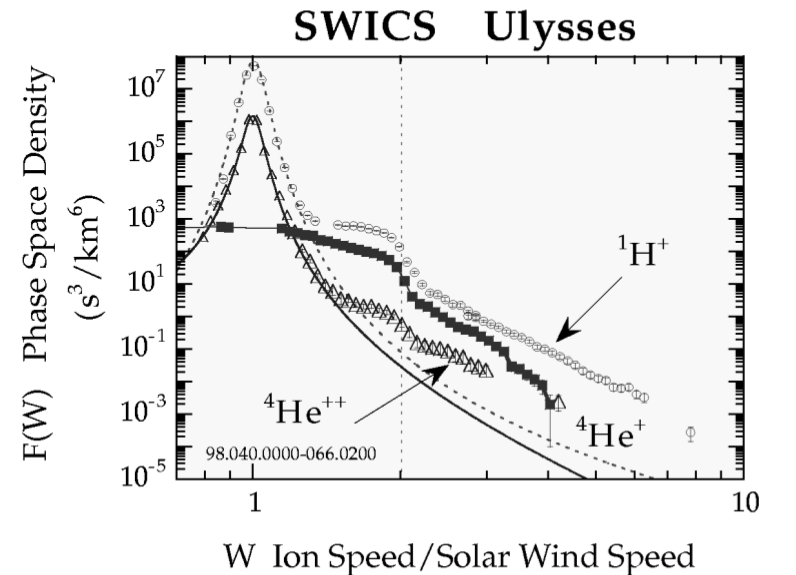
\includegraphics[width=0.8\textwidth]{Figures/sw_pui_gloeckler.png}
	\centering
	\caption{Phase space density for $\mathrm{He^{2+}}$, $\mathrm{He^{+}}$ and $\mathrm{H^{+}}$ against $w = \frac{v_\mathrm{ion}}{v_\mathrm{sw}}$ in the slow solar wind ($v_\mathrm{sw} = 375\,\mathrm{km\,s^{-1}}$). PUI distributions are clearly visible for all three species in the $w$ range between $\sim$ 1.5 and 2 followed by a cutoff at $w = 2$ and high-velocity tails. Solar wind distributions are represented by the dashed and solid curves for $\mathrm{He^{2+}}$ and $\mathrm{H^{+}}$. The figure is taken from \citet{gloeckler1999}.} 
	\label{fig:gloeckler}
\end{figure}
Many studies on PUI VDF base on measurements of Ulysses/SWICS \citep[s.][]{gloeckler_geiss}.
These studies were limited to 1D reduced observations in the spacecraft frame until today, as only the absolute values of velocities were considered.
An example by \citet{gloeckler1999} is shown in Fig. \ref{fig:gloeckler}. Here we see the phase space density of three different pickup ion species drawn against $w$, which is the ion's velocity divided by the current solar wind speed. The pickup ions shows a non-Maxwellian distribution with a clear cutoff at w=2. While the distributions of He2+ and H+ are superimposed by the distribution of the solar wind ions around w=1, the distribution of He+ PUI is unveiled.  
However, the actual PUI VDF is multi dimensional and cannot be reproduced from the reduced 1D measurement without making assumptions on the underlying distribution.
Several 3D VDF may lead to the same 1D VDF when being reduced and thus every 1D measurement is ambiguous.

As Ulysses SWICS is capable of resolving the inflow direction of incident ions, a three dimensional VDF can be obtained when taking into account all given information.
The aim of this thesis is to make use of this information and to develop a tool to provide three-dimensional VDFs. 
PUI differ from solar wind ions by a non-Maxwellian VDF. As this distribution is particularly broad, He+ PUI are the perfect candidates for testing the tool and for being studied with it.
\\
The thesis starts with an introduction into PUI, before the Ulysses mission and the instrument SWICS with its measurement principle are described. In the third chapter a virtual detector is developed to translate the raw He+ data into three dimensional velocity components. For this, SWICS' intrigue geometry has to be considered as well as Ulysses' orientation in space and its eigen-velocity. In the final section the obtained three dimensional spectra are presented in different projections.



%%%
%-------------------------------------------------------------
%%%

10% Chapter 1

\chapter{Pickup Ions} % Main chapter title

\label{chapter:theory} % For referencing the chapter elsewhere, use \ref{Chapter1} 

%-------------------------------------------------------------



%-------------------------------------------------------------

Pickup ions are created when neutral atoms inside the heliosphere become ionised and are subsequently swept away with the heliospheric magnetic field that is embedded within the solar wind.


\section{The Heliosphere / Introduction}

Oder Überkapitel Solar Physics?
\\ \\
Heliosphere: Grenze zu LISM
\\ \\
Solar Wind: Zusammensetzung, schneller und langsamer, high latitudes: less complex, constant in speed \\ \\
B-Feldgleichung
\\ \\
Irgendwohin muss unbedingt Motivation, warum PUIs überhaupt interessant sind zu messen!
\\
PU Process
%%%
%-------------------------------------------------------------
%%%

\section{Pickup Ions}
A neutral atom inside the heliosphere is only subjected to the gravitational force and radiation pressure of the sun. It is not sensitive to any electromagnetic forces until it becomes ionised by solar ultra-violet radiation, charge exchange with solar wind protons or electron impact (Q?). After ionisation the particle starts interacting with the solar wind plasma. In particular it is forced onto a gyro orbit about the heliospheric magnetic field
that is embedded within the solar wind. As the freshly created ion is swept away with the magnetic field line it is \say{picked up} from its location of ionisation -- a new pickup ion (PUI) has been created.
\\ \\
PUIs were first observed by \citet{moebius_nature_85} with the SULEICA Instrument on the AMPTE spacecraft. The particles measured at $1\,\mathrm{AU}$ were He+ ions of interstellar origin.
\\ \\
Once the particle is ionised, its probability to become ionised another time decreases (Quelle). This characteristic of being only singly charged can help to discriminate PUIs from solar wind ions, that are mostly more often charged (Q?).
\\ \\
PUIs are mostly only single charged. This characteristic can help to distinguish them from solar wind ions of coronal origin which often have been ionized multiple times, if not completely. (Q?)
\\
VDF non-maxwellian, spatial density pattern 
\\ \\
There have been observed several species of PUIs: 
\section{Interstellar Pickup Ions}
Heliosheath, relative motion \\ \\
The neutral part of the LISM can enter the heliosphere as it is not affected by the heliosheath (Todo). Inside the heliosphere the neutrals are guided only by the gravitational force and raOriginofC-Geissdiation pressure of the sun. The neutral particle's species determines how deep it can travel into the heliosphere before it becomes ionized. Species with a higher First Ionization Potential will be able to approach the sun much closer without being ionized. This results in He+ being the dominant PUI species at a solar distance of $1\,\mathrm{AU}$ even if in the LISM the abundance of hydrogen is about 10 times the one of helium.
\begin{itemize}
	\item ionisation process is also dependent on the species
	\item radiation pressure only important for H (and He?). Kepler orbit...
	\item Spatial distribution:\\
	gravitational force and radiation pressure lead to two regions of enhanced density of neutrals (in the ecliptic): Focusing cone and crescent.
	Focusing cone: For species with high FIP (as the others are ionized before and do not reach the downwind side of the sun)
	\item variation of He+ with the solar cycle: Rucinski 2003
	\item H, O and N are depleted in the filtration region (Baranov Malama 1995), Wimmer Skript: even before ioniztion: density is determined by ratio of gravitational force and photon pressure
	\item neutral density determines PUI production rate
\end{itemize}

\section{Inner-source Pickup Ions}
The idea of an additional source for the PUI's neutral seed population was born when \citet{geiss_1995a} measured a global distribution of C+ PUIs with the SWICS instrument on Ulysses. 
Interstellar carbon exists almost exclusively in a single charged state \citep{Frisch} in the LISM. As only neutral atoms can enter the heliosphere it was not expected to find a distinct signature of C+ pickup ions.
However, pickup carbon was observed with about the same ratio as oxygen, of which, in contrast, ~80\% is in a neutral charge state in the interstellar medium.
These findings suggested that there must be another source for neutrals that has its origin somewhere inside the heliosphere. \\
In following studies \citep[e.g.][]{geiss_1995b} there were found also other species like O+ and Ne+ of these, so called, inner-source PUIs.
\\
Inner-source PUIs show a composition that is similar to the one of the solar wind \citep{gloeckler2000_innersource, allegrini_2005} as well as a velocity distribution function that is centered around $w_{SC} \approx 1$ \citep{schwadron_2000} and seems to have thermalized with the solar wind.
\\
Beneath those two characteristics there are other aspects concerning inner-source PUIs, that are still under debate. In particular that is the production mechanism of their neutral seed population.
\citet{allegrini_2005} has summarized current candidates for possible scenarios. Two of those give an explanation for the ion's composition as they directly incorporate solar wind ions in the process:
\begin{itemize}
	\item Solar wind recycling \citep{gloeckler2000_innersource, schwadron_2000}: Absorption of solar wind ions by heliospheric grains and subsequent reemission of neutral atoms
	\item Solar wind neutralization \citep{wimmer_2002}: Solar wind ions penetrate sub-micron-sized dust grains and undergo (partial) neutralization by charge exchange
\end{itemize}
(As this work does not focus on inner-source PUIs in particular...)


\section{VDF}
After the particle has been ionised it is forced onto a gyro motion about the local field line of the heliospheric magnetic field due to the Lorentz force. 
\\ \\
To examine the velocity distribution of PUIs after they have been ionized we need to consider the initial speed $v_{ini}$ of the neutral particle. 
For neutrals from the LISM this is mainly given by the inflow speed $v_{ISM}$ of the local interstellar medium with which they enter the heliosphere. As we don't exactly know about the production mechanism of inner-source PUIs, the following considerations mainly relate to interstellar PUIs.
\citet{schwadron_2015_ibex} obtained $v_{ISM} \approx 25 \,\mathrm{km\,s^{-1}}$ with the IBEX satellite for helium. Considering the acceleration by the sun's gravitational force we have a maximum initial speed of $v_ini \approx 50 \,\mathrm{km\,s^{-1}}$ at $1\,\mathrm{AU}$. Compared to an average solar wind speed of $v_{sw} \approx 400\,\mathrm{km\,s^{-1}}$ one can neglect this initial speed in a first step.

For simplicity we thus consider a neutral particle at rest that becomes ionized by one of the aforementioned processes. The freshly created ion now is subjected to the electromagnetic forces of the solar wind plasma. In particular, it finds itself at a velocity $v_{sw}$ relative to the magnetic field which is convected outwards by the solar wind that is assumed to flow radially outwards. Due to the Lorentz force the PUI starts to gyrate about the magnetic field line on an orbit that is perpendicular to it. \\
When we further consider a magnetic field's orientation that is perpendicular to the solar wind flow, $\vec{B} \perp \vec{v}_{sw}$, the ion's gyration speed is $v_{sw}$ while its guiding center moves together with the field line at a speed of $v_{sw}$ as well.
Thus, the total speed of the PUI ranges between $0\, \mathrm{v_{sw}} $ and $2 \, \mathrm{v_{sw}}$ in a sun frame of reference. \\
As the heliospheric magnetic field lines are shaped like an Archimedean spiral, the so called \textit{Parker spiral}, the assumption of a perpendicular magnetic field only applies when solar wind speed $v_{sw}$ and solar distance $r_\odot$ follow the relation
\begin{align*}
90 ^\circ \approx  arctan \left( \frac{2\pi}{T_\odot \cdot v_{sw}} r_\odot \right)
\end{align*}
with sun's sidereal period $T_\odot \approx 25\,d$ \citep{prlss_2004}.
In other cases, e.g. for solar distances about $1\,\mathrm{AU}$, at which the angle between solar wind and magnet field direction is approximately $45^\circ$, the maximum speed in a sun frame of reference is decreased. In general, the gyration speed is given by
\begin{align*}
todo
\end{align*}
with ... .
\\ \\
The velocity space for a pickup situation with a non-radial magnetic field orientation is shown in figure todo on the right.
The PUI's total velocity consists of the movement of the guiding center (...) and the gyration velocity (...). We note, that in this case there is a relative velocity between the motion of the solar wind bulk and the PUI's guiding center movement. 
\\
However, independent on the magnetic field orientation, every possible velocity space trajectory is part of a sphere with the radius $v_{sw}$ centered around $\vec{v}_{sw}$. That means that, in the frame of the solar wind, the freshly created PUI always moves with a speed that is as fast as the solar wind itself. (todo: Hier w einführen?) 
\\ \\
Instead of a single PUI we can consider an ensemble of PUI's that is injected into the solar wind while the magnetic field orientation is not changing much. For that we expect the VDF to form a ring shape in velocity space, commonly called the "PUI torus VDF" \citep{oka_2002}.
The expected orientation of this highly anisotropic torus VDF depends on the local magnetic field direction and is sketched in figure todo for three different angles.
\\ \\
...thickness that is related (associated) to the neutral's velocity and is very small compared to the radius...\\ \\
Spatial diffusion: chalov Fahr 1998. Signature of plasma parcel in which is was produced doesn't match with the one it is measured in
\\ \\
After the injection, the PUI population is radially carried away with the solar wind. During phase space transport through the heliosphere the PUIs are subjected to multiple processes that are expected to modify the shape of the initial toroidal VDF. However, it is not completely understood how the VDF evolves in detail.
\\ \\
A fast isotropization of the VDF due to pitch-angle scattering was suggested by \citet{vasyl_siscoe_1976} in a theoretical work.
However, observations by e.g. \citet{moebius_98} on $He+$ or \citet{gloeckler_1995} on TODO have shown clear anisotropic features in the measured VDFs.
Following studies (todo) explained these findings with the assumption that the ions would be injected into the sunward hemisphere of velocity space more likely. Ineffective pitch-angle scattering into the antisunward hemisphere thus would result in an radial anisotropy.
\\ \\
Recent observations have emphasized the influence of the magnetic field direction on the measured anisotropy.
Utilising 2D analyses of the velocity space, \citet{oka_2002} and \citet{drews_2015} found that the measured VDF of PUIs is systematically oriented about the direction that is perpendicular to the magnetic field.
Thus, it is believed that the VDF's anisotropic features are remnants of the initial toroidal VDF. (and the pa scattering didnt have enough time to isotropize the distribution)
\\ \\
Furthermore, there are different acceleration and deceleration processes that change the PUI's initial VDF and lead to a diffusion in velocity space.
Under the assumption of an isotropic VDF the PUI population is often treated as an adiabatic gas that is consequently cooled when expanding with the solar wind. This picture, initially suggested by \citet{vasyl_siscoe_1976}, however, must be reviewed due to the doubtful fact of a fully isotropic VDF.
Another cooling mechanism, called the \textit{magnetic cooling}, is due to the magnetic field weakening with solar distance. As the PUIs are swept outwards both their ... and their ...invariant have to be conserved which leads to a decrease in both velocity components (parallel and perpendicular to the magnetic field) and thus to a decrease in total velocity (in the frame of the solar wind).
\\ \\
(focusing (adiabatic invariant) \& Ginzberg Landau (Fahr2008): "magnetic cooling" (auch gute Erklärung: Fahr\&Fichtner2011))
\\ \\
Acceleration of PUIs can be caused by 
acceleration: first and seconf order fermi (verstehen, gründe): eher außen bzw. ehr innen. Außerdem ein Mechanismus, der nicht an einzelne Events gebunden ist, sondern immer vorhanden: Mechanismus für alle Teilchen, power law -5...\\
man kann in der 1D Verteilung beobachten, dass 2vsw exceeded wird
\\ \\
PUI He should be measured throughout the mission as they penetrate the heliosphere until 0.5 AU \citep{gloeckler_1992}
\\ \\ \\
Instrument that is capable of measuring this distribution: large acceptance in absolute velocity, large variation and resolution in angles
\subsection{1D reduced VDF, aim of this work...?}
% Chapter Template

\chapter{Instrumentation} % Main chapter title

\label{chapter:instrumentation} 

%----------------------------------------------------------------------------------------

%----------------------------------------------------------------------------------------

\section{Ulysses}
\label{sec:ulysses}
The Ulysses spacecraft \citep{wenzel_ulysses} was launched in 1990 and orbited the sun for nearly 20 years as a joint ESA/NASA project.
Ulysses' most remarkable feature is its out-of-ecliptic orbit with a maximum heliographic latitude of $80.1\,^\circ$.
As the first spacecraft it was hence capable of taking in situ measurements from above the poles of the sun.\\
The primary goal of the mission was to study the heliosphere in three dimensions. Some of the original main objectives were:
\begin{itemize}
	\item to study the interplanetary magnetic field and the solar wind, especially its composition, the origin and waves and shocks within the solar wind plasma
	\item to investigate galactic cosmic rays and energetic particles
	\item to improve the knowledge about interplanetary dust
	\item to explore the neutral component of interstellar gas
\end{itemize}
Some secondary objectives included e.g. the investigation of Jupiter's magnetosphere during the Jupiter flyby and the search for gravitational waves and for gamma-ray burst sources \citep{wenzel_ulysses}.
\\
For these aims Ulysses was equipped with a wide range of different instruments and antennas. One of the in situ instruments is the Solar Wind Ion Composition Spectrometer (SWICS), that will be described in the next section.\\
A sketch of Ulysses' unique orbit is shown in figure \ref{fig:trajectory}.
Ulysses was launched in October 1990 and left earth's gravitational field with $15.4\,\mathrm{km/s}$. Starting with a flyby manoeuvrer around Jupiter Ulysses was sent onto its highly elliptical orbit.
With an orbital period of 6.2 years Ulysses completed nearly three orbits around the sun until communication was shut down in June 2009 due to the expiring of the radioisotope thermal generators.
Within the mission's long lifetime the Sun's behaviour over its activity cycle of 22 years could be studied.\\
Ulysses is a spin-stabilized spacecraft that spun at $5\,\mathrm{rpm}$. The spin axis is aligned with the high-gain antenna's electrical axis, that provided a communication link from the spacecraft to Earth. The downlink bitrate was variable with up to $1024\,\mathrm{bit/s}$ during real-time connection.
\\ \\ 
TODO: Importance PUIs?
\begin{figure}[h]
	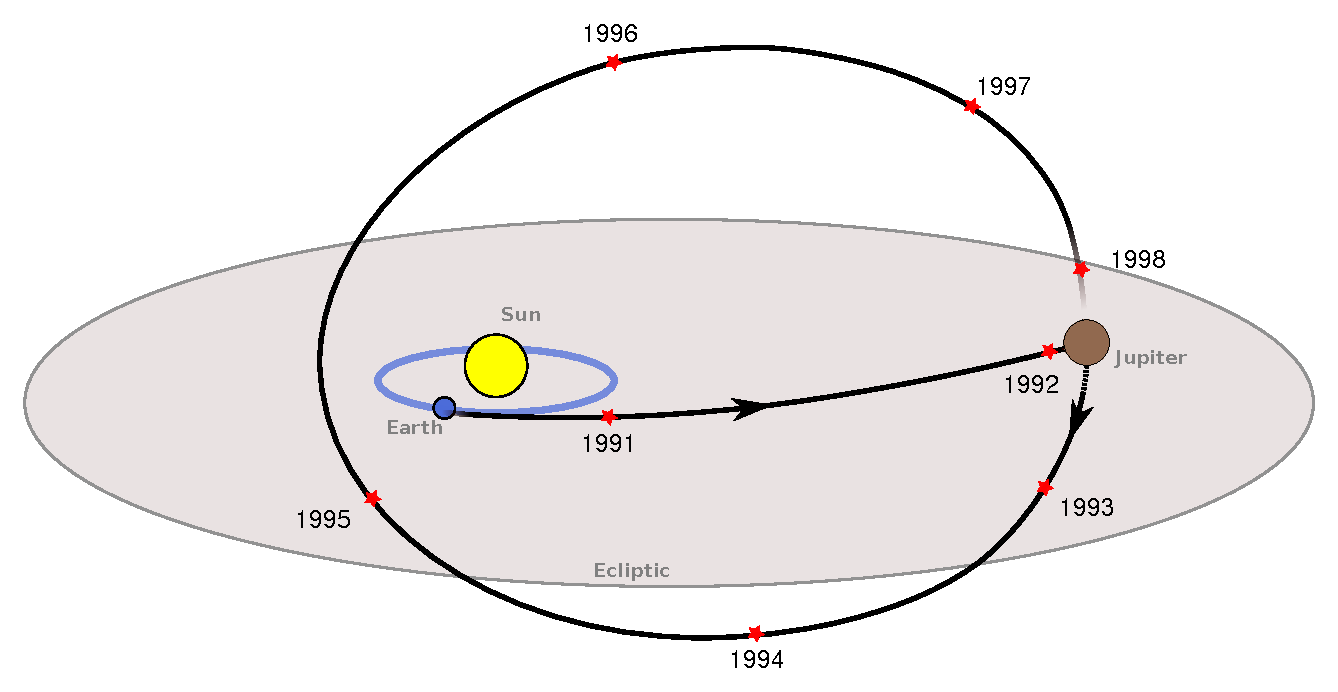
\includegraphics[width=0.8\textwidth]{Figures/ulysses_trajectory.pdf}
	\centering
	\caption{A sketch of Ulysses' first orbit. After the launch from earth in 1990 the spacecraft was sent to Jupiter from where it left the ecliptic on an elliptical orbit around the sun with perihelion at $1.3\,\mathrm{AU}$ and aphelion at $5.4\,\mathrm{AU}$. Due to the orbit's high latitude of $\sim 80 \, ^\circ$ Ulysses crossed the Sun's pole regions two times between 1994 and 1996. Figure after \citet{esa_orbit}.}
	\label{fig:trajectory}
\end{figure}
%
%
%
%
%
\section{SWICS}
\label{sec:swics}


\begin{figure}
	\centering
	\begin{subfigure}{.5\textwidth}
		\centering
		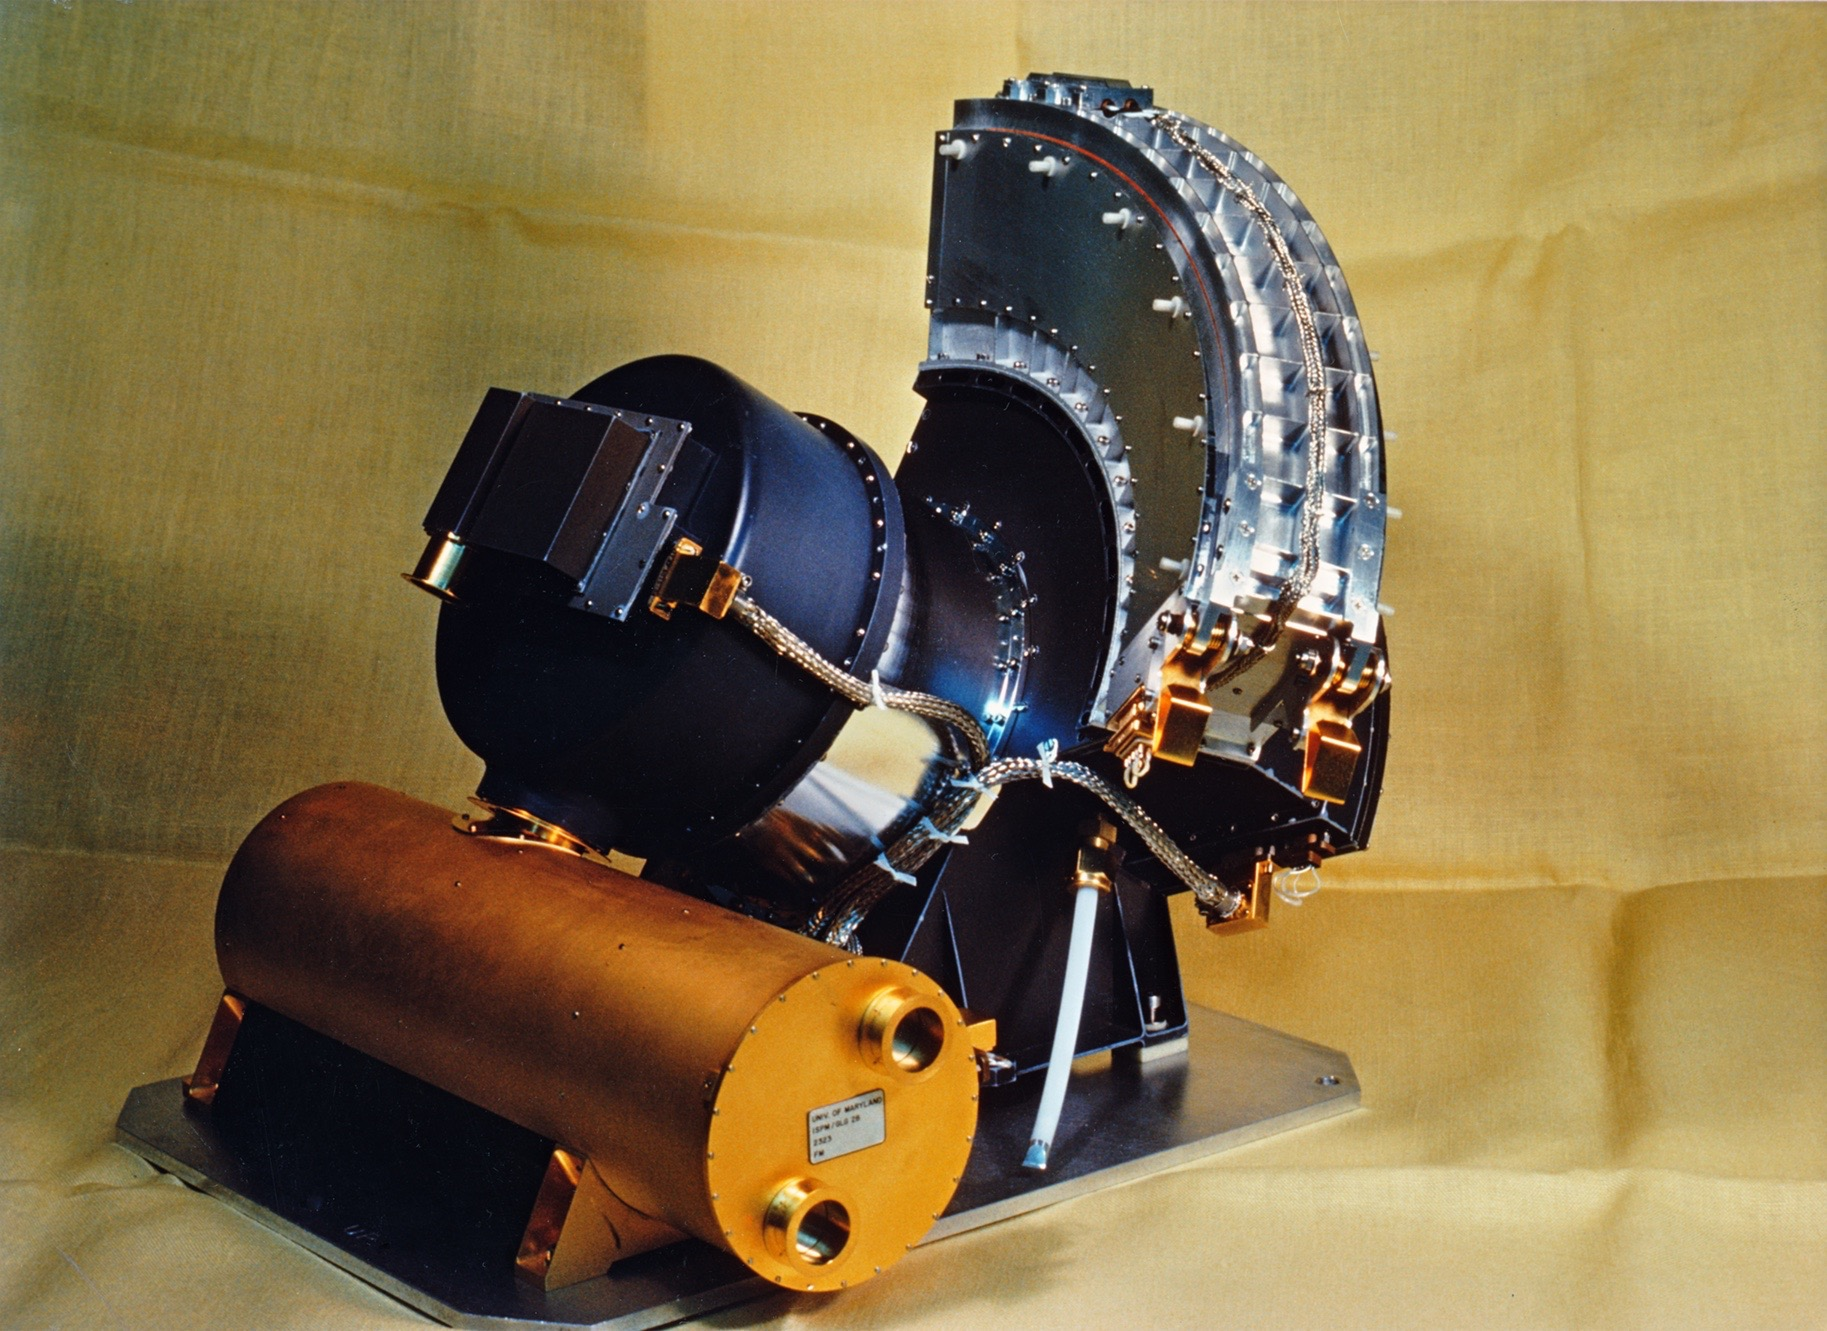
\includegraphics[width=0.9\linewidth]{Figures/ULYSSES-SWICS.jpg}
	\end{subfigure}%
	\begin{subfigure}{.5\textwidth}
		\centering
		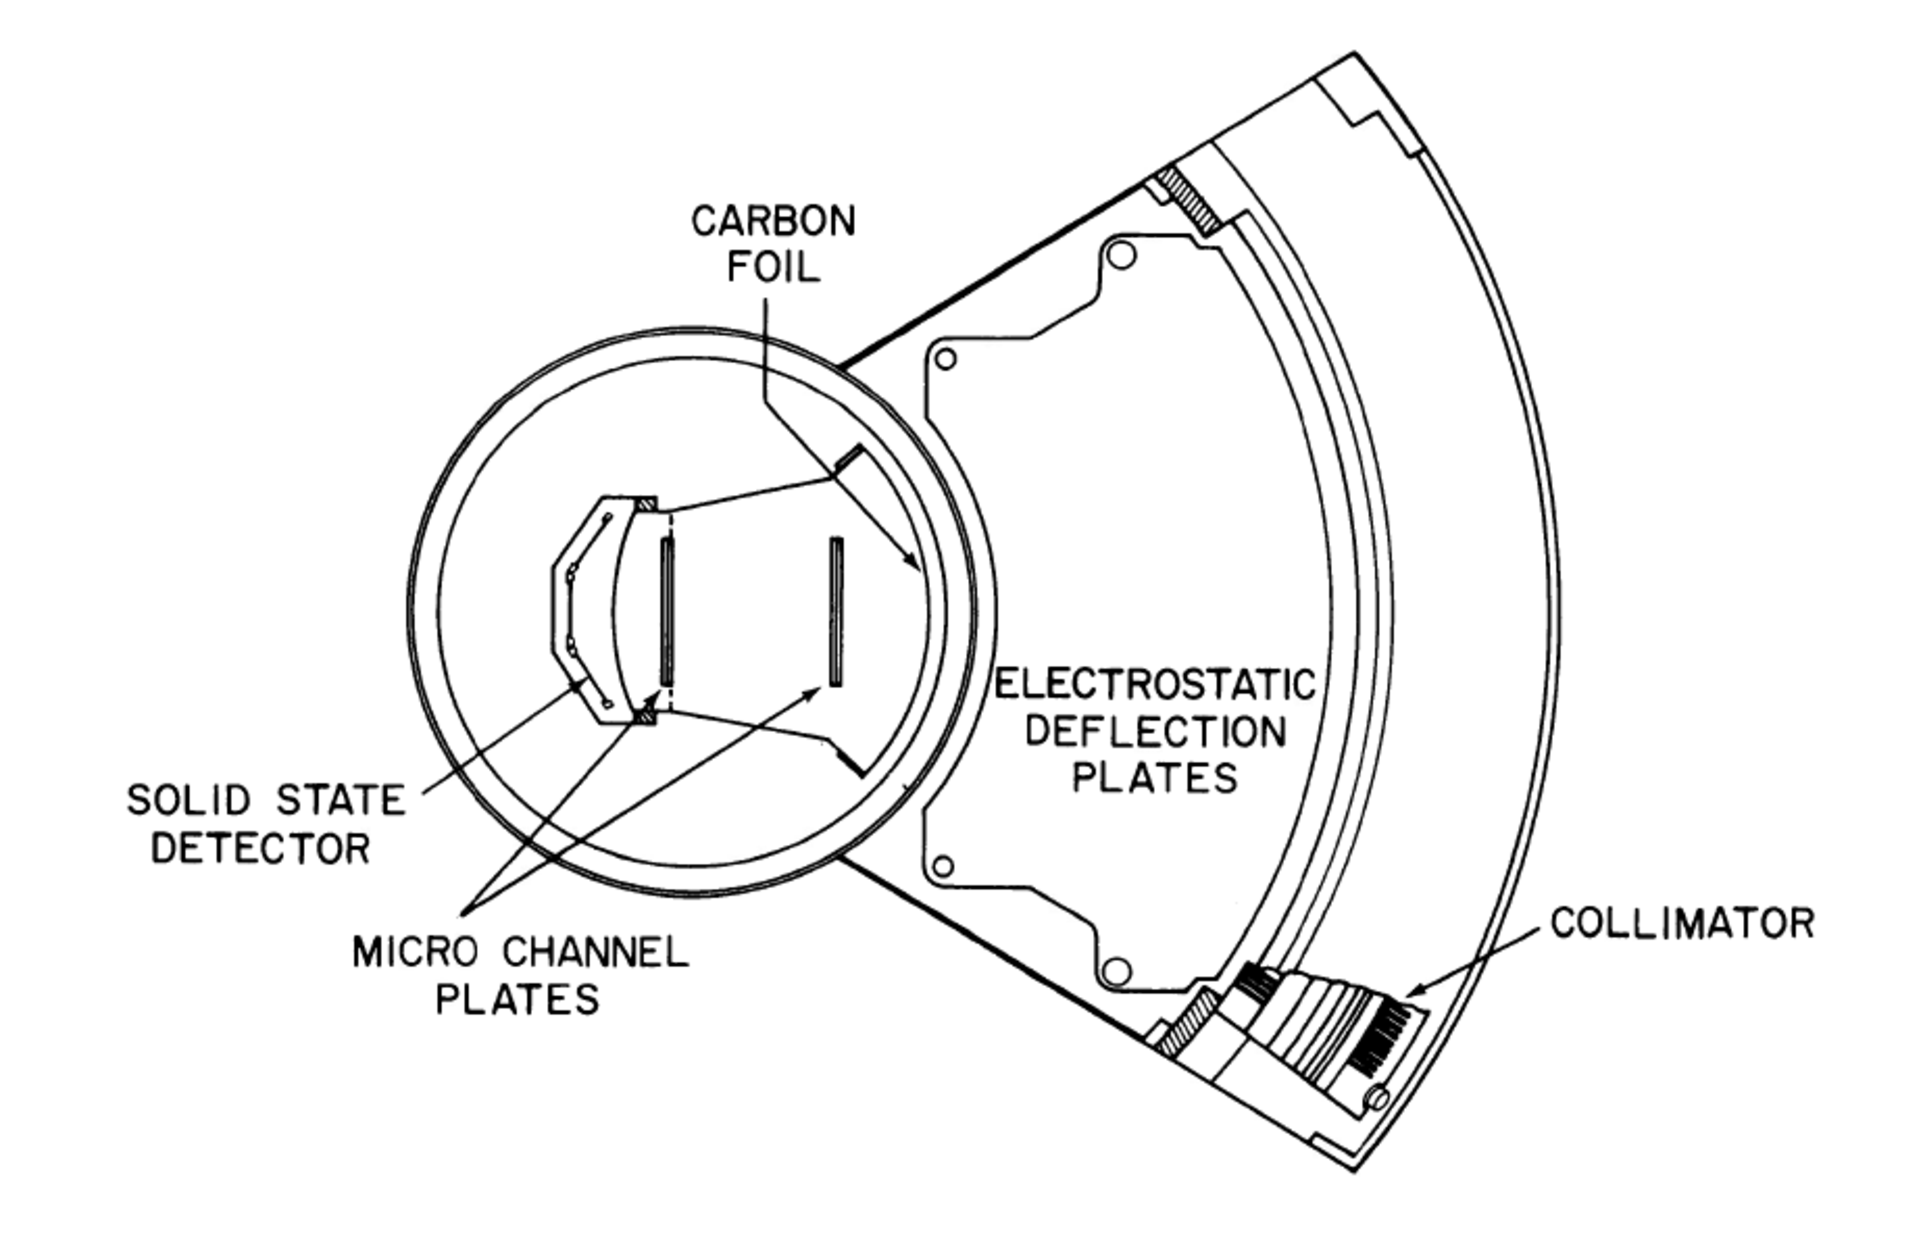
\includegraphics[width=1.1\linewidth]{Figures/swics_sensor.pdf}
	\end{subfigure}
	\caption{\\ \textit{Left:} Photograph of the SWICS instrument. The fan-shaped collimator on top of the electrostatic deflection analyzer can bee seen on the right. It is followed by the cylindrically shaped and silvery coloured \textit{high-voltage bubble}, that contains the time-of-flight system, analog electronics and and the sensor power supply. The gold-plated cylinder houses a $-30\,\mathrm{kV}$ voltage supply. The opening angles of the collimator are $69^\circ$ in width and $4^\circ$ in height. OPT: Ausschneiden und beschriften \\ \textit{Right:} Schematic cut through the sensor. In this view the orientation of the three solid state detectors is visualized. OPT: farbig markieren\\ Both figures are from from \citet{gloeckler_1992}.}
	\label{fig:swics}
\end{figure}

The Solar Wind Ion Composition Spectrometer (SWICS, \citet{gloeckler_1992}) is a time-of-flight mass spectrometer mounted on the spacecraft Ulysses (s. sec. \ref{sec:ulysses}). The instrument is designed to determine the elemental and charge-state composition and the velocity distribution of solar wind ions. With an energy-per-charge range from $0.16 \, \mathrm{kV}$ to $59.6 \, \mathrm{kV}$ SWICS is able to measure every solar wind ion species from protons to iron with any typical charge state. Depending on the individual ion, particle energies from $1 \,\mathrm{keV}$ up to $1 \, \mathrm{MeV}$ are covered.\\
SWICS is mounted on the sun-facing side of Ulysses and revolves around the spacecraft's spin axis with the spacecraft spinning. A photograph of the instrument is shown in fig. \ref{fig:swics}, left.\\
Ulysses SWICS also has a twin instrument that is the SWICS spare model, which has been mounted on the ACE spacecraft \citep{stone_ace}.
\\ \\ 
TODO: Super für measuring PUIs! viele wichtige Messungen... \\ \\
%
%
%
SWICS measures the mass $m$, the charge $q$ and the energy $E$ of entering ions by a combination of three separate measurements: The electrostatic deflection analyzer within the entrance systems is used for determining the energy-per-charge of a particle. Within the time-of-flight/energy section the particle's time-of-flight and residual energy are measured. A more detailed description of the measurement is given in the next sections. A particle's trajectory through the instrument can be tracked in the schematic in fig. \ref{fig:lars_swics}.
%
\subsection{Collimator and Electrostatic Analyzer}
\label{sec:EpQ}
Particles enter the instrument through the entrance collimator. It restricts particles to the ones with a trajectory that is parallel to the collimator slits.  The collimator follows an intricate geometry that is fan-shaped with an opening angle of $69^\circ$ in width and $4^\circ$ in height and that is at the same time curved along its width. Fig. \ref{fig:swics}, left,  gives an idea of the shape.\\
After having entered through the collimator a particle has to pass the electrostatic analyzer. It is split up into two sections -- energies-per-charge from $0.16$ to $14\,\mathrm{kV}$ are covered by the proton/helium channel. Particles within this range of energy will be filtered by their energy-per-charge and after an post-acceleration will be counted by a solid-state detector. As this simple measurement principle is very limiting for our analysis we will focus on the main channel that is suitable for a full \textit{mass/mass-per-charge} analysis.\\
The main channel covers an energy-per-charge range of $0.66$ to $60.51\,\mathrm{kV}$. A particle can only pass through the pair of curved deflection plates if its kinetic energy-per-charge equals a certain ratio that is given by the voltage between the two plates. To measure particles of different energy-per-charge the deflection voltage is stepped through 64 logarithmically spaced values, s. fig \ref{fig:epq}. As the voltage steps once per spin of Ulysses (every $12\,\mathrm{s}$), a complete voltage cycle lasts $\sim$ 12.8 minutes. 
Every step has a relative uncertainty in energy-per-charge of $\Delta \mathrm{EpQ / EpQ = 5\%}$  that is due to the finite space between the plates.
%
%
%
\begin{figure}[h]
	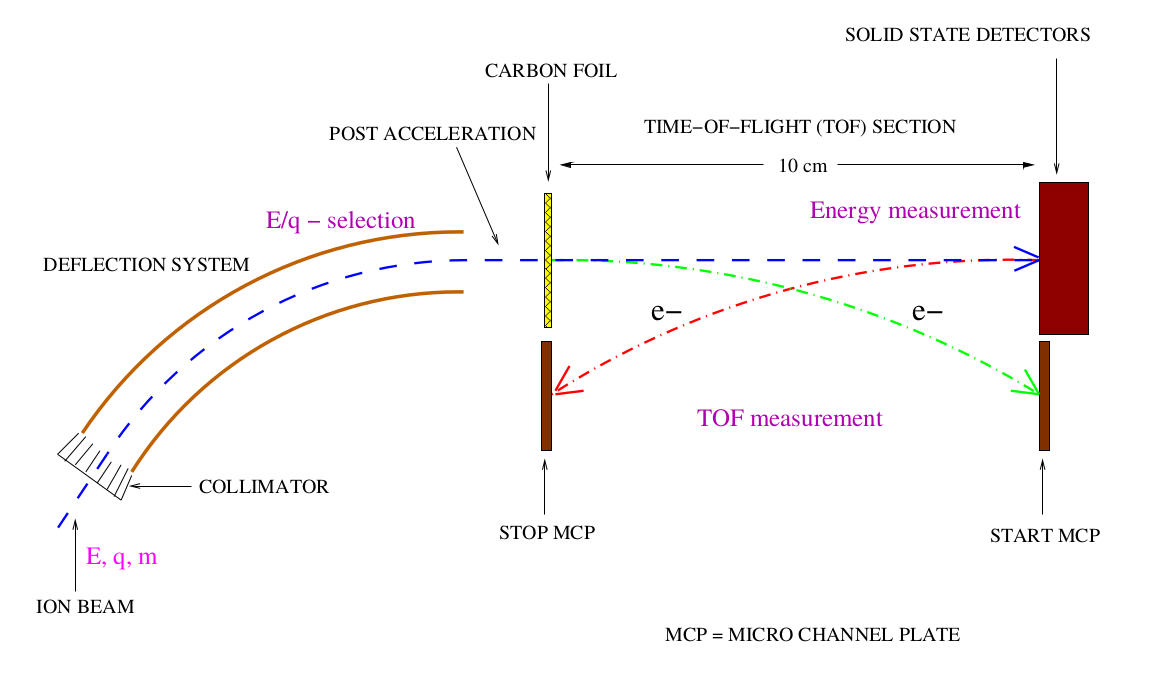
\includegraphics[width=0.8\textwidth]{Figures/Lars_Swics.png}
	\centering
	\caption{Schematic view of the SWICS detector. See text for reference. This figure is taken from \citet{lars-phd}.}
	\label{fig:lars_swics}
\end{figure}

%
\begin{figure}[h]
		\centering
		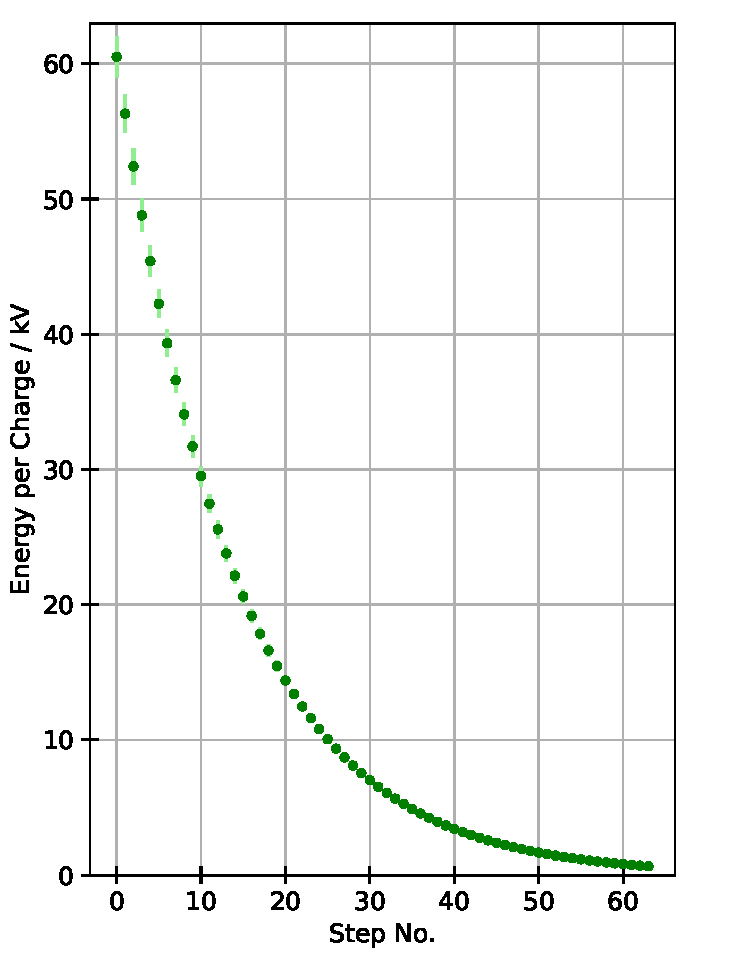
\includegraphics[scale = 0.7]{Figures/epq_err.pdf}
		\caption{Energy-per-Charge steps of Ulysses SWICS. A voltage cycle starts with step 0 that is the highest voltage $EpQ = 60.51\, \mathrm{kV}$. Voltage is then swept down 64 logarithmically spaced steps up to $EpQ = 0.66\, \mathrm{kV}$. The uncertainty of the single steps is $\frac{\Delta EpQ}{EpQ} = 5\%$ and drawn in lighter color.
		} \label{fig:epq}
\end{figure}
%
%
%
\subsection{Time-of-flight measurement}
After having passed the electrostatic analyzer the ion is post-accelerated by an constant potential drop of ~$30\,\mathrm{kV}$. It enters the time-of-flight chamber with penetrating through a thin ($\sim 3\,\mu \mathrm{g / cm^2}$) carbon foil from which secondary electrons are emitted. These electrons are guided to a microchannel plate detector where a start signal is triggered (s. fig \ref{fig:lars_swics}). The stop signal is triggered after the ion has traversed nearly force free a distance of $10\,\mathrm{cm}$ through the vacuumized time-of-flight section. Here it hits one of the solid-state detectors, where secondary electrons are emitted again. By combining the times of the start and the stop signal the particle's time-of-flight has been measured.
\subsection{Energy measurement}
Additionally, the ion's energy is measured when they hit one of the three solid state detectors. \\
A solid-state detector is realized by applying an inverse bias voltage to a semiconductor material. When ionized particles hit the material, they set free charge carriers from the resulting depletion zone. These charge carriers can be measured as a pulse of current which is proportional to the deposited energy of the ion. \\
Each of the three detectors has an active area of $1.5 x 1.3 \,\mathrm{cm^2}$. Their alignment with each other can be seen in fig \ref{fig:swics}, right: While the central detector is oriented perpendicular to the symmetry axis of SWICS, the other two detectors are slightly tilted with respect to this axis. This way particles with different angles of incidence along the width of the collimator can be detected. The information on which of the three detectors has been hit will be utilized in chapter \ref{chapter:data} for a coarse directional resolution of incident particles.
\\ \\
One of SWICS' main objectives is the measurement of the composition of incident particles. An ion and its charge state can be fully identified with the knowledge of its mass $m$ and its mass-per-charge $mpq$. 
With the measurement of the time-of-flight $ToF$, the energy $E_{SSD}$ and the knowledge of the energy-per-charge $EpQ$ we can calculate the mass $m$, the mass-per-charge $mpq$ and velocity $v$ of an ion $i$ with the following set of equations:
\begin{align}
m_i &= 2\,E_{SSD} \left( \frac{Tof}{d}\right)^2 \label{eq:swics_set1}\\
mpq_i &= 2 \left(EpQ + V_{PAC}\right) \cdot \left(\frac{Tof}{d}\right)^2 \label{eq:swics_set2} \\
v_i &= \sqrt{2\,EpQ\,\frac{1}{mpq_i}},
\label{eq:swics_set3}
\end{align}
where $d$ is the length of the time-of-flight section and $V_{\mathrm{PAC}}$ is the post-acceleration voltage. $v$ denotes the ion's initial velocity when entering the instrument and is not to be confused with its velocity during the time-of-flight measurement, that is altered particularly by the post-acceleration.
%
%
%
\section{Data products}
\label{sec_dataprod}
Direct Pulse-Height Analysis data (PHA data) are one of SWICS' data products and the ones that are most relevant for the analysis in this work.\\
Over one voltage cycle SWICS steps through the 64 energy-per-charge steps of the electrostatic analyzer (s. sec \ref{sec:EpQ}), which we call ESA steps. At normal spacecraft telemetry rates SWICS steps once per spin, which is once every $12\,\mathrm{s}$. During these times 30 PHA words per spin are selected and transmitted. The selection is based on a priority scheme that is described below in sec. \ref{subsec:prio}.\\
Every 24-bit PHA word contains following information on an incident particle that triggered a valid measurement:
\begin{itemize}
	\item $E_{SSD}$: Energy deposition in the solid state detector \\
	measured through 256 channels in a range $40 - 600\,\mathrm{keV}$
	\item $ToF$: Time-of-Flight\\
	measured through 1024 channels in a range $10 - 200\,\mathrm{ns}$
	\item Sector information:\\
	SWICS divides one spin of Ulysses up into 8 sectors of approximately equal duration. This yields in information on the spatial origin of particles.
	\item Detector information: \\
	Which of the three solid state detector elements has been triggered?
	\item Priority category: \\
	Due to limited telemetry only an assorted sample of all measured particles can be transmitted. This selection is based on different priorities. For details s. sec \ref{subsec:prio}.
\end{itemize}
The interpretation of a set of PHA words that have been collected over time is discussed in sec. \ref{sec:etmatrices}. 
%
\subsection{Detection Efficiency}
\label{subsec:det_eff}
When working with SWICS -- like for any physical measurement -- one has to consider several constraints that impede the ideal measurement as it is described in sec. \ref{sec:swics}. \\
One of these constraints is the detector efficiency, which describes the probability to measure a particle that has entered the instrument (Todo: ?). 
With an ion passing through the time-of-flight section there is the likelihood that secondary electrons may not be emitted properly from the carbon foil and solid state detector which then leads to an invalid time-of-flight measurement. Also, ions could pass through the time-of-flight section on divergent trajectories due to scattering processes (TODO: in the carbon foil??). Subsequently, the ion possibly does not hit the sensitive area of the solid state detector and would neither trigger a stop signal for the time-of-flight measurement nor a valid energy measurement in the solid-state detector.\\
Another reason for an invalid energy measurement in the solid-state detector can be that the ion's energy is smaller than the threshold of the solid-state detector. In this case, only energy-per-charge and time-of-flight information for the ion are available. Such events without a corresponding energy measurement are called double coincidences, while events with triggered start and stop signal and an energy measurement are called triple coincidences.\\
The reason for choosing a non-zero threshold is to limit the influence of the solid-state detector's natural noise. For SWICS this noise level is quite high, at around $12\,\mathrm{keV}$ \citep{gloeckler_1992} (todo: ?), so that the threshold is chosen to be $\sim 30 \, \mathrm{keV}$. 
The detection efficiency is highly dependent on the ion species and deflection step.
Ions with a small mass and charge are most likely to not overcome the threshold at low energy-per-charge values. For the bulk of $\mathrm{He^{+}}$ this is already the case for ESA step 17 ($EpQ = 17.86\,\mathrm{kV}$), which corresponds to a $\mathrm{He^{+}}$ velocity of $v = 900\,\mathrm{km\,s^{-1}}$ (s. eq. \ref{eq:swics_set3}).\\
Unfortunately, $\mathrm{He^{+}}$ detection efficiencies are not known to us for Ulysses SWICS. Instead, we make use of the efficiencies from ACE SWICS, that have been calculated by \citet{koeten}. As ACE SWICS uses different energy-per-charge ranges we had to extrapolate the values for Ulysses SWICS.
For the highest energy-per-charge value $EpQ = 60.51\,\mathrm{keV}$ we interpolated the efficiency from the ACE $\mathrm{He^{+}}$ triple efficiencies and then extrapolated linearly to an efficiency of 0 at ESA step 17. By this, we accommodate for the above mentioned fact that $\mathrm{He^{+}}$ does not have enough energy to deposit energy above the solid state detector's threshold at ESA step 17 and thus, the probability for a triple coincidence is zero. $\mathrm{He^{+}}$ efficiencies from ACE SWICS and the resulting efficiencies used for Ulysses SWICS are shown in fig. \ref{fig:guess_eff}. For sure, these values are not realistic but represent the overall trend of a decreasing efficiency for higher ESA steps.
\begin{figure}[h]
	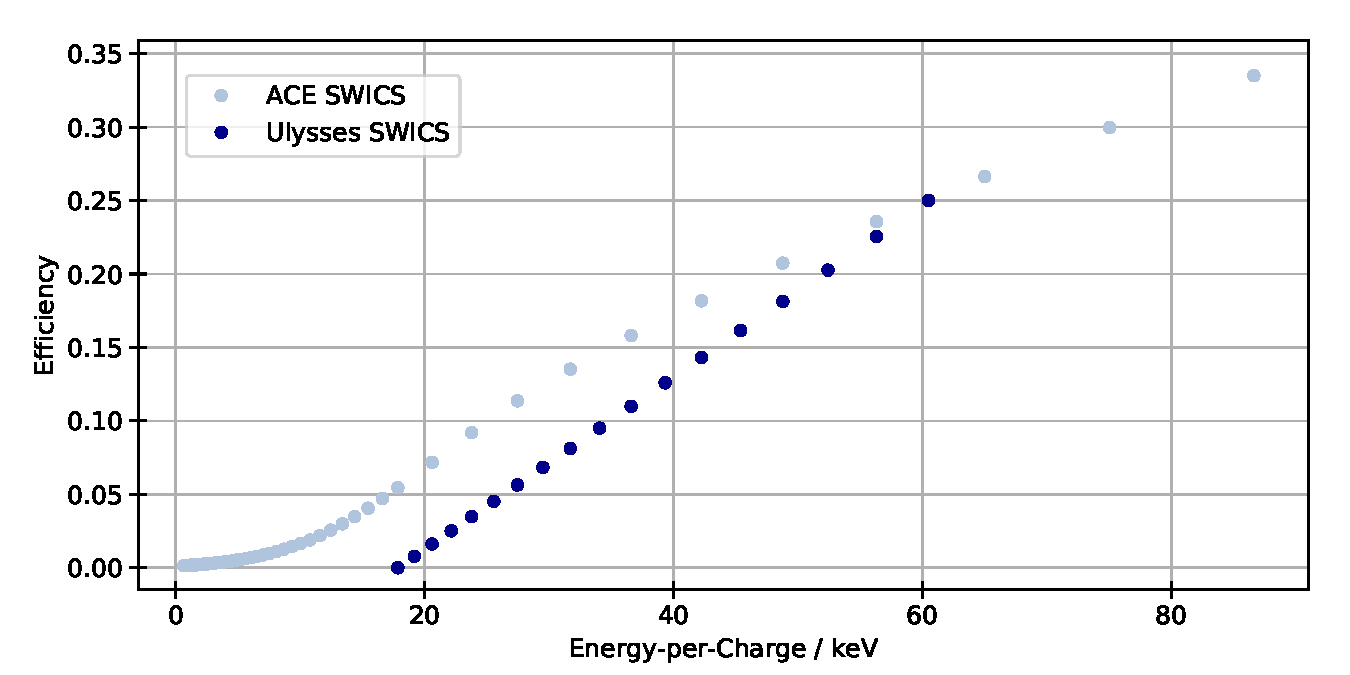
\includegraphics[width=1.\textwidth]{Figures/guess_eff.pdf}
	\centering
	\caption{$\mathrm{He^{+}}$ detection efficiencies for ACE SWICS over all ESA steps from $0.66\,\mathrm{kV}$ to $86.64\,\mathrm{kV}$. For Ulysses SWICS the efficiencies have been extrapolated between 0 for ESA step 17 ($EpQ = 17.86\,\mathrm{kV}$) and the highest efficiency for ESA step 0 ($EpQ =60.51\,\mathrm{kV}$). The latter value has been interpolated from the ACE efficiencies.}
	\label{fig:guess_eff}
\end{figure}


\subsection{Priority Weighting}
\label{subsec:prio}
SWICS' data processing unit performs an on-board mass and mass-per\--charge-clas\-sification. For every ion with valid measurements the mass $m$ and mass-per-charge $mpq$ are calculated based on the measurements of $E_{\mathrm{SSD}}$, $ToF$ and the particle's ESA step using a look-up-table technique.\\
On the one hand these values are used for sorting the ions into predefined boxes in the $m$-$mpq$-space which yield in the so-called matrix rate, a second data product that is provided benath the PHA words.\\
Secondly, and more important for our analysis, the m and mpq information is used to sort every measured ion into one of three priority ranges. Due to a limited telemetry possibly not every measured particle can be transmitted as a PHA word. 
30 PHA words per spin are chosen from these ranges in way that the ratio of low and high priority PHA words is balanced. By this selection less abundant heavier ions are artificially enhanced which is necessary to recreate the measured composition from the transmitted PHA words. Table \ref{tab} shows a summary of this priority scheme. Details about this can be found in \citet{gloeckler_1992}.\\
To account for the priority biased selection of PHA words it is necessary to weight the transmitted data with the so-called base-rate weight $brw = \frac{D_{\mathrm{PHA}}}{T_{\mathrm{PHA}}}$, where $T_{\mathrm{PHA}}$ is the number transmitted PHA words and $D_{\mathrm{PHA}}$ the number of detected particles on which this PHA word is based. The measured composition can be restored in this way.
\begin{table}[h]
	\caption{SWICS' priority categorization scheme} 
	\centering
	\begin{tabular}{c|c|c}
		%\hline
		Range 0 & $m < 8.7$;  $m_0 : mpq < 3.3$ & $\mathrm{H}$, $\mathrm{He^+}$, $\mathrm{He^{2+}}$; Doubles\\ 
		\hline 
		Range 1 & $m > 8.7$ & Heavier ions \\ 
		\hline 
		Range 2 & $m_0 : mpq > 3.3$ & Doubles \\ 
		%\hline 
	\end{tabular} 
	\label{tab}
\end{table}
%
%
%
\section{ET matrices, identification}
\label{sec:etmatrices}
Fig. \ref{fig:et_matrix} shows longterm PHA data collected over two years with Ulysses SWICS for ESA step 24 ($EpQ = 10.8\,\mathrm{kV}$). For every particle with valid time-of-flight and energy measurements the $E_{\mathrm{SSD}}$ channel is plotted over the time-of-flight channel. As a particle's mass and mass-per-charge are connected to the measured values $EpQ$, $ToF$ and $E_{\mathrm{SSD}}$ by equations \ref{eq:swics_set1} --  \ref{eq:swics_set3}, every ion species occupies a distinct position in this histogram, which we call ET-matrix. 
However, due to uncertainties in the measurements of $EpQ$, $ToF$ and $E_{\mathrm{SSD}}$ an event may be displaced around its ideal position. 
For multiple events of the same species this results in broadened distributions. A detailed discussion on these uncertainties can be found for example in \citet{lars-phd}.
We can identify several ion species in the shown ET-matrix: A selection of those is labelled in \ref{fig:et_matrix}.



\begin{figure}[h]
	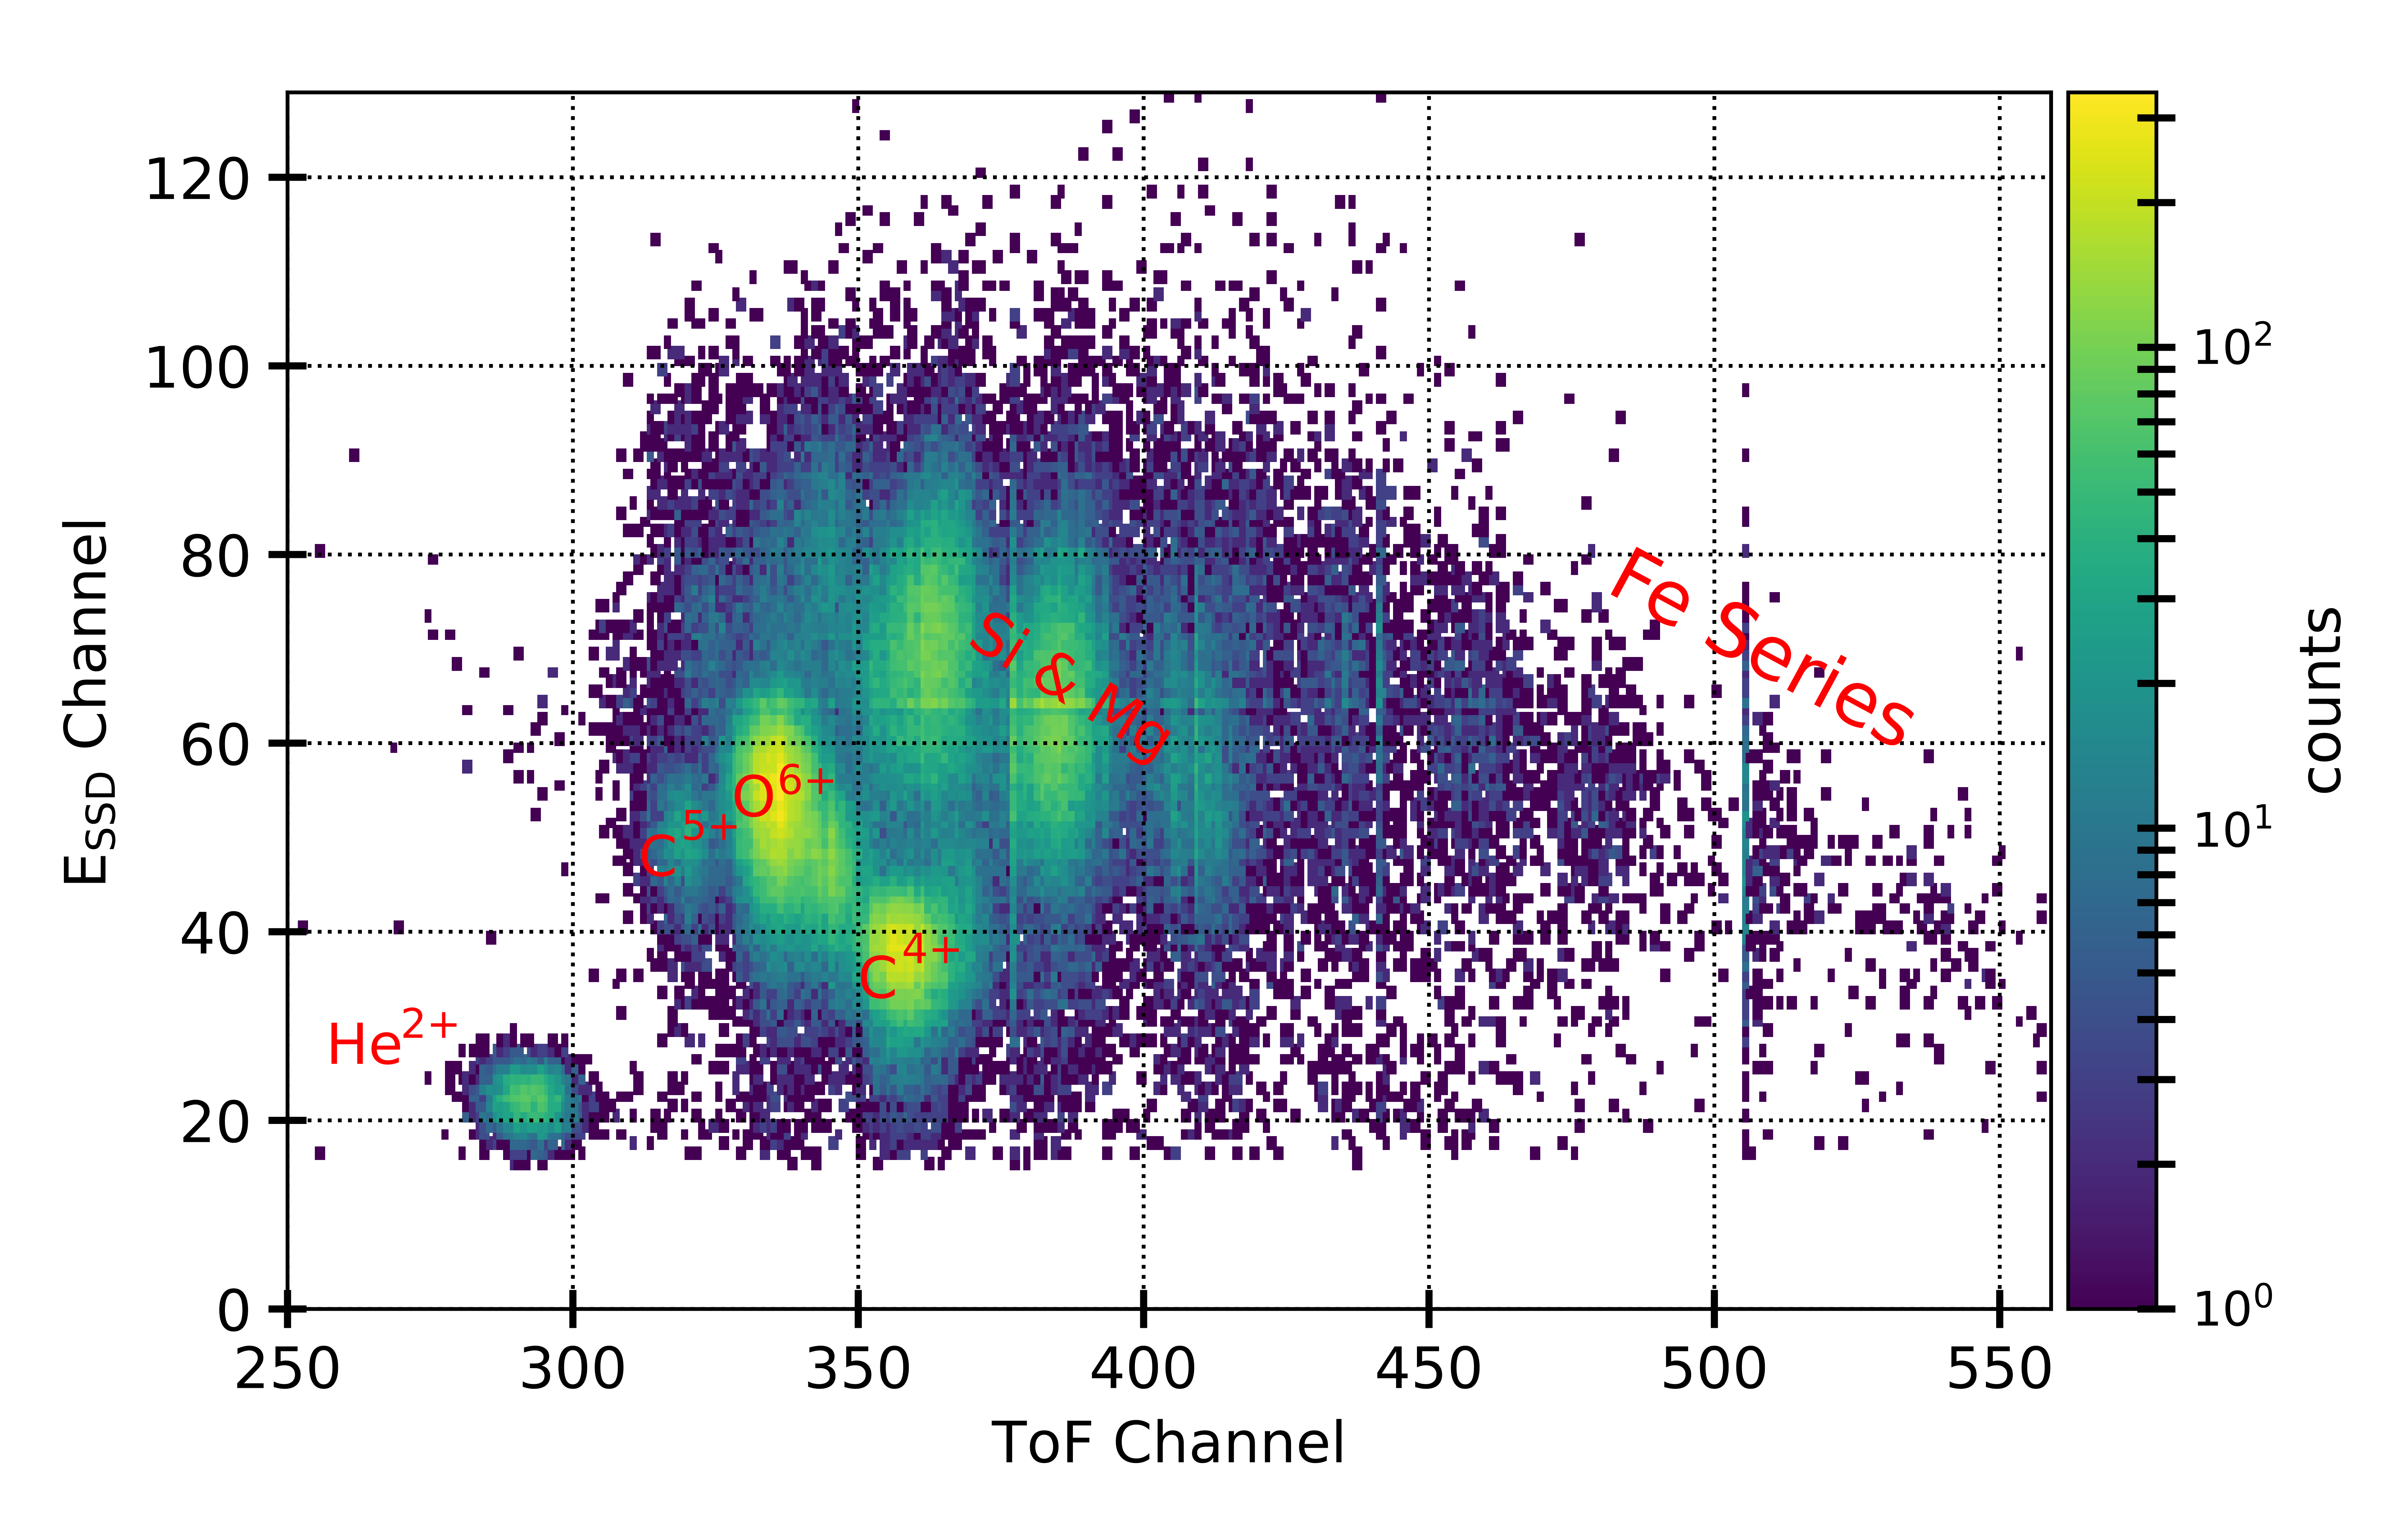
\includegraphics[width=0.9\textwidth]{Figures/et_matrix_labels.png}
	\centering
	\caption{ET-matrix from Ulysses SWICS PHA data of years 1993-1994. All plotted events were measured during ESA step 24 ($EpQ = 10.8\,\mathrm{kV}$). Only triple coincidences are shown. Besides accumulated counts in ion-specific positions, there are a few horizontal and vertical stripes apparent in the shown ET-matrix -- for example in $E_{SSD}$ channel 65 and time-of-flight channel 409, 377 or 505. These are imprints of irregularities within SWICS' Analog-Digital-Converters which can be noticed as a saturation of one bin while the adjacent bin is depleted. However, these signatures are not expected to have a significant effect on the following analysis.}
	\label{fig:et_matrix}
\end{figure}


\subsection{Selection of $\mathrm{He^{+}}$}

\begin{figure}[h]
	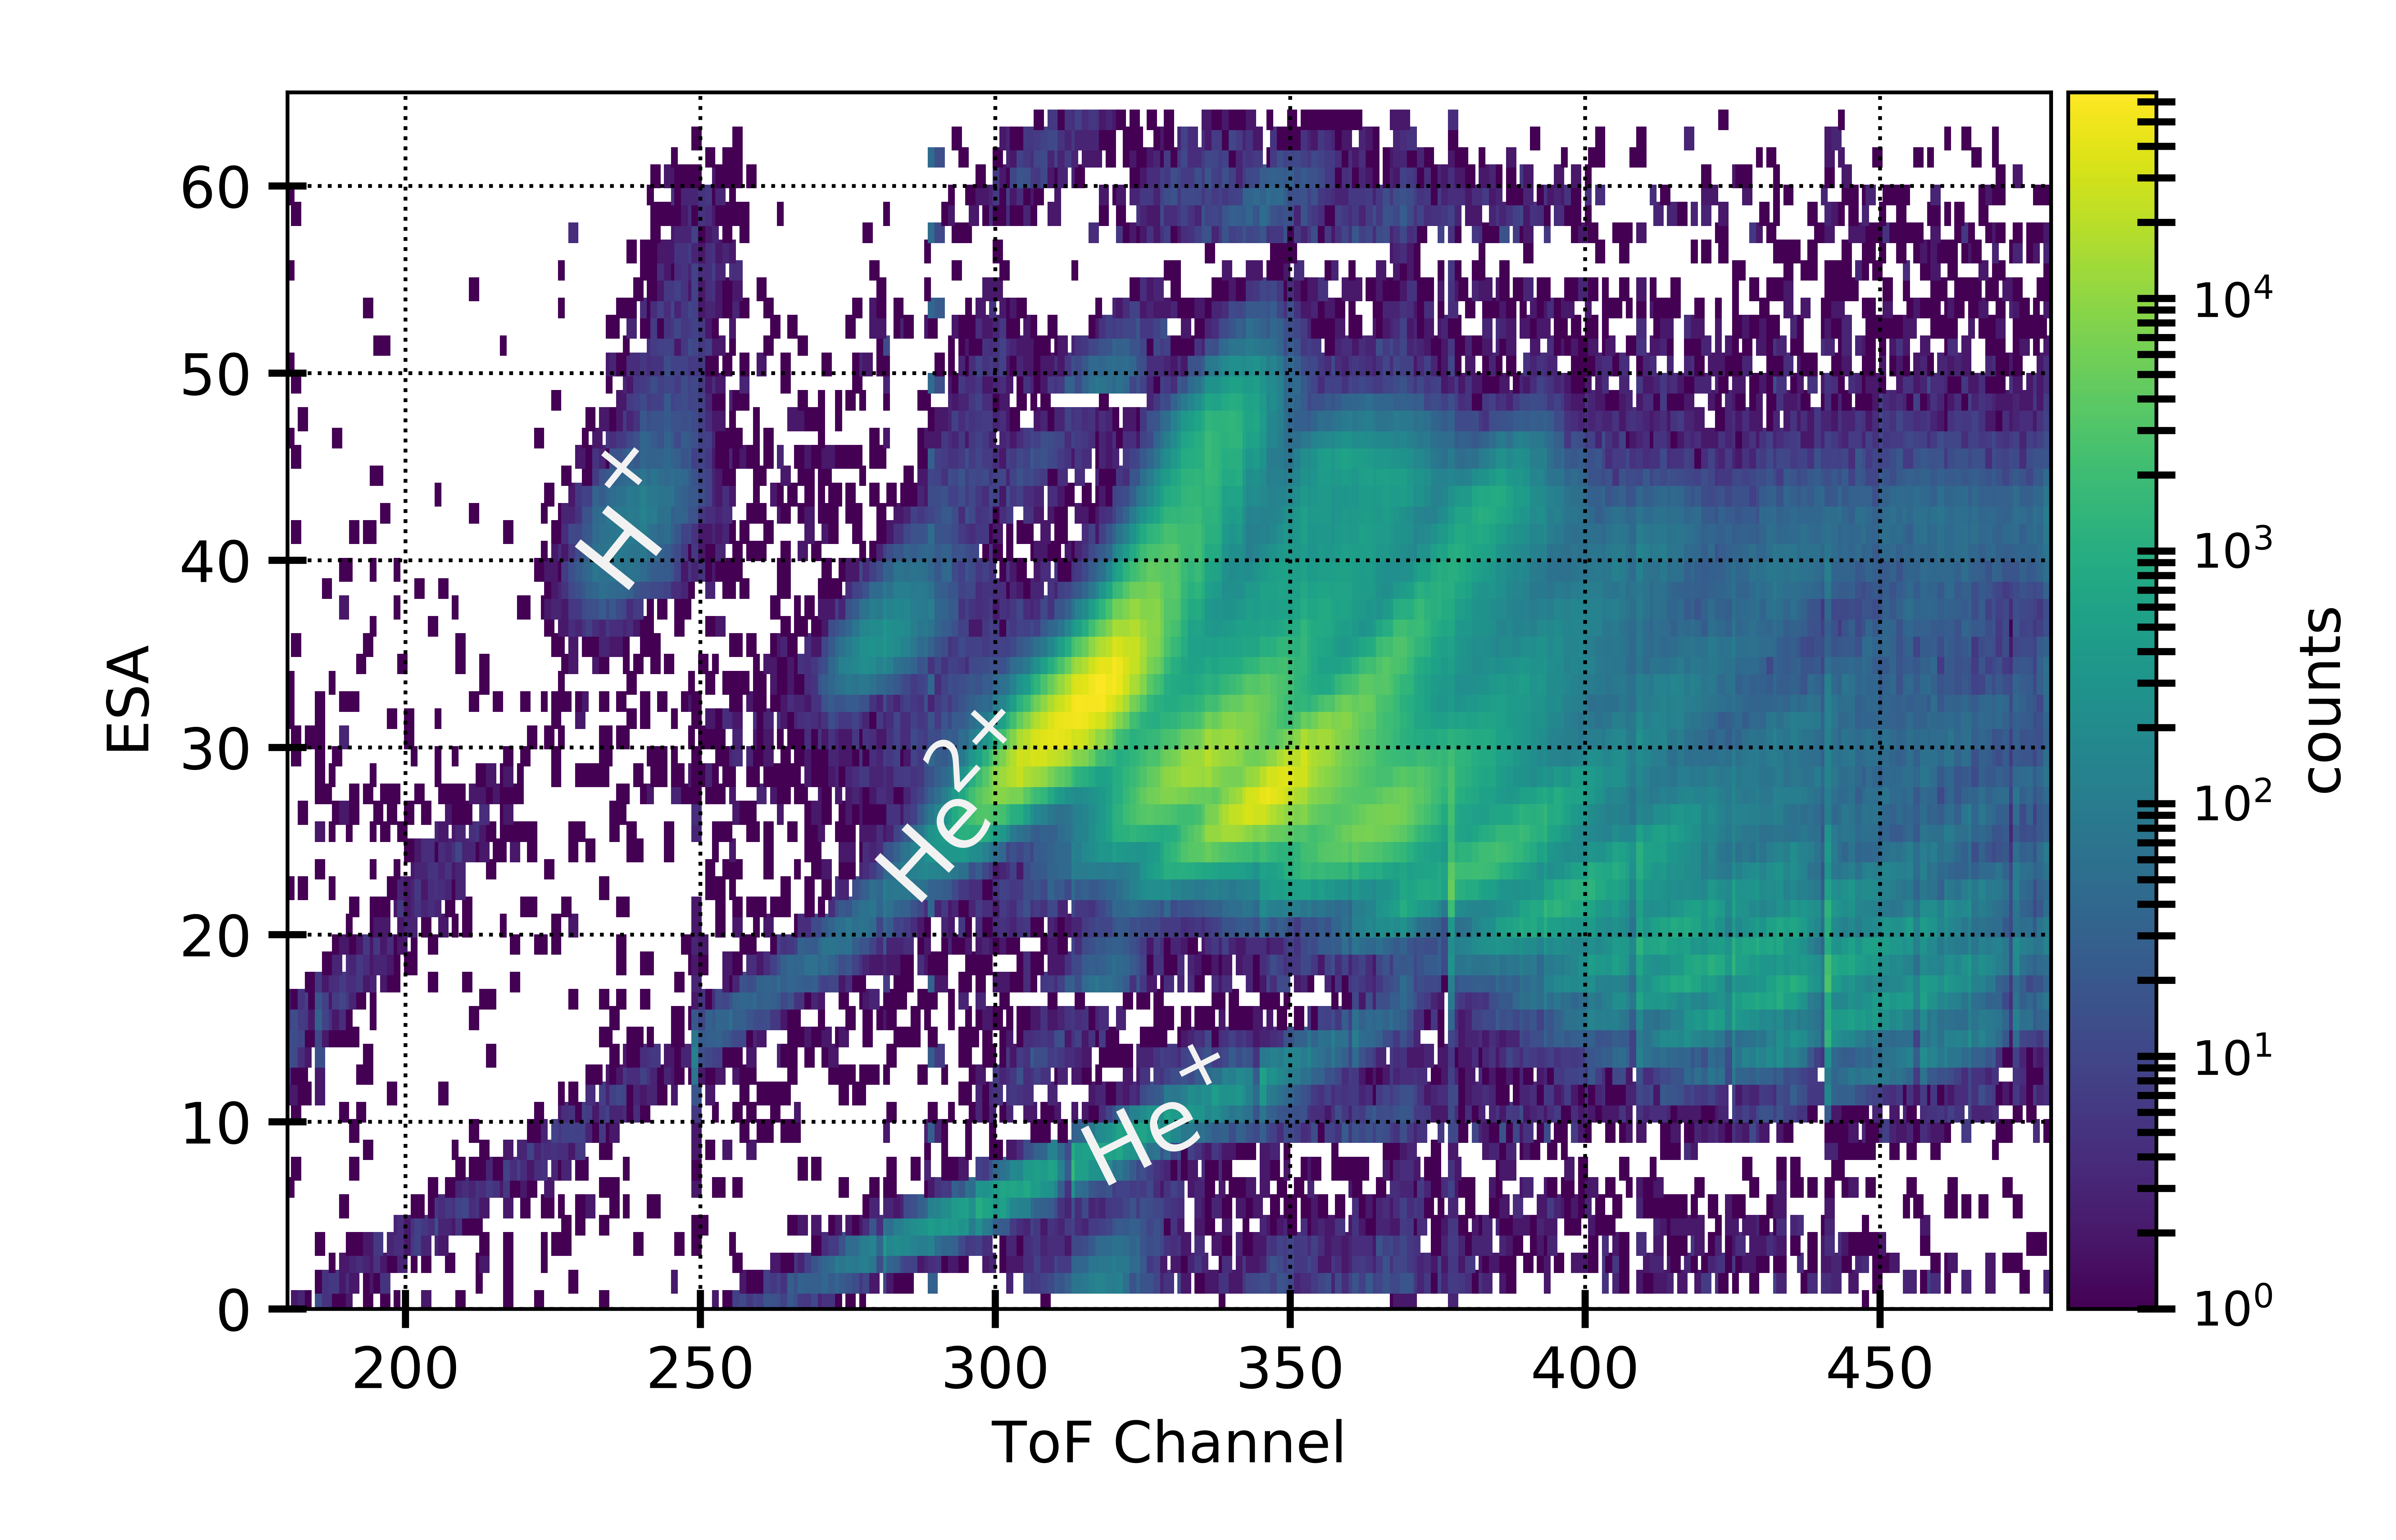
\includegraphics[width=0.9\textwidth]{Figures/epq_all.png}
	\centering
	\caption{Histogram over time-of-flight and ESA channels of two years (1993-1994) of Ulysses SWICS Triple Coincidence PHA data. Note, that the ESA channel numbers are inversely proportional to the energy-per-charge values. Ion species with the same mass-per-charge ratio can be detected on curves $ESA \sim ToF^2$.}
	\label{fig:epq_all}
\end{figure}

\begin{figure}[h]
	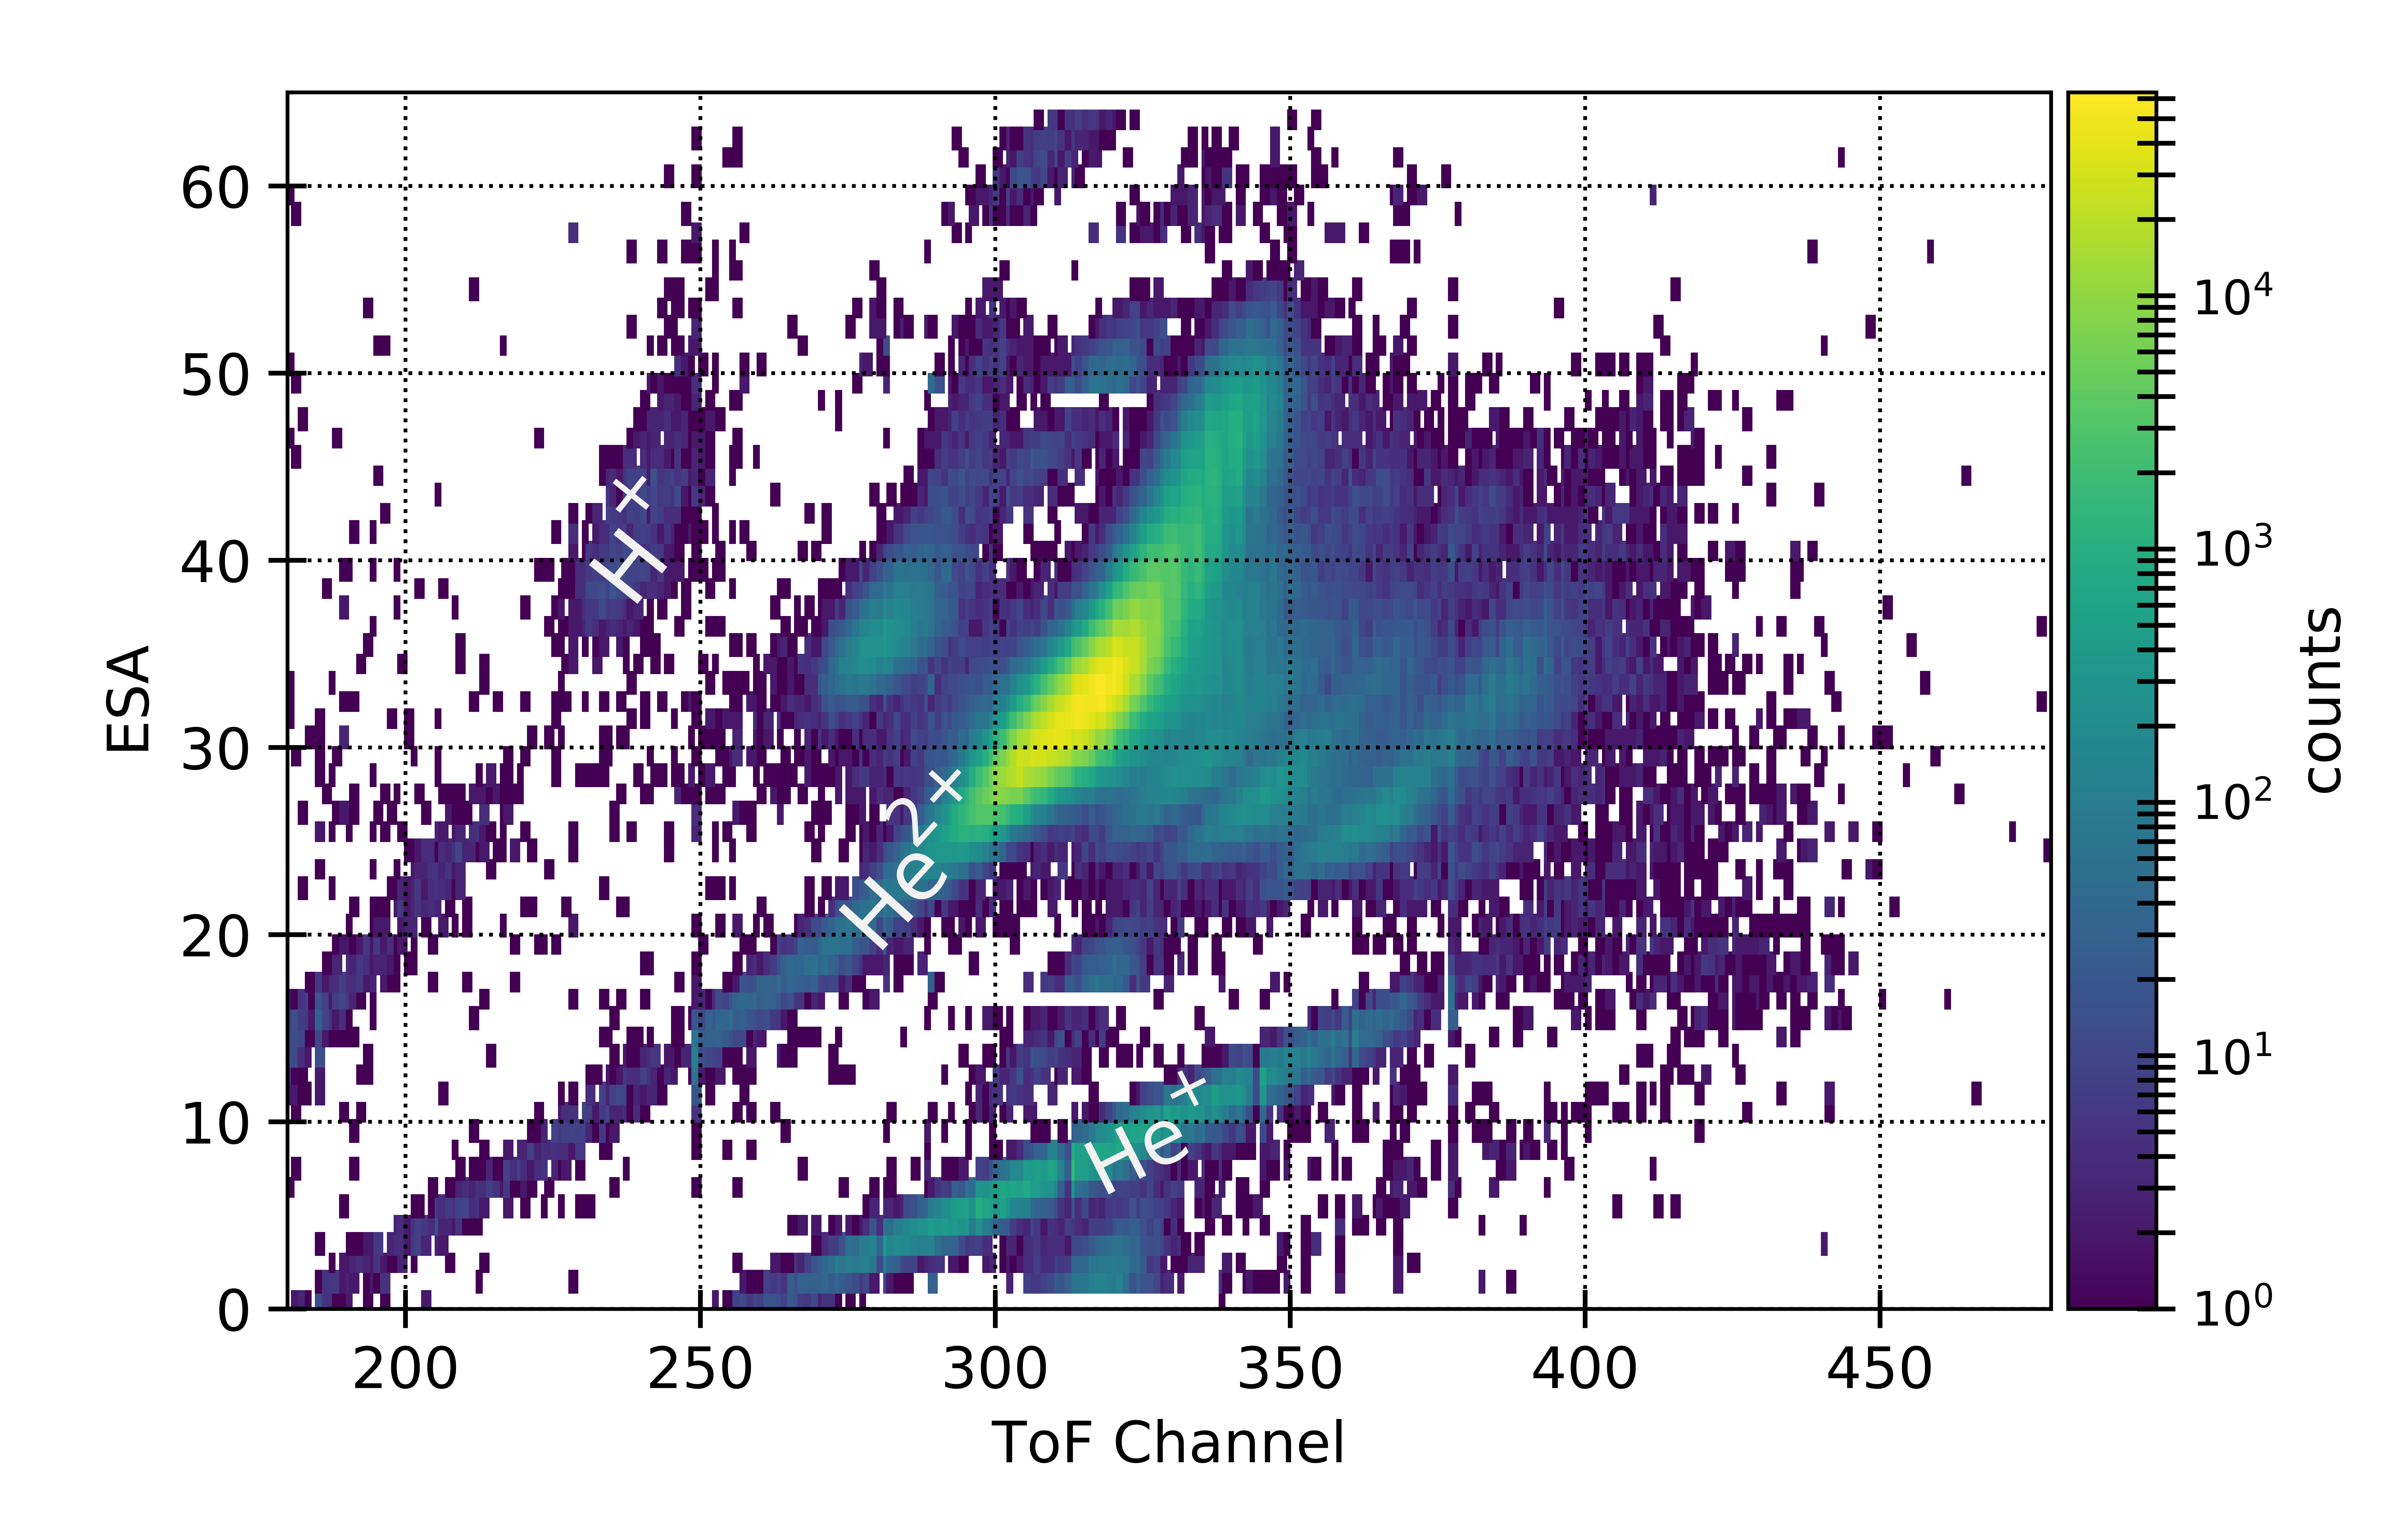
\includegraphics[width=0.9\textwidth]{Figures/epq_rng0.png}
	\centering
	\caption{The same histogram as in fig. \ref{fig:epq_all}, but this time only events with Range-0 priority are plotted. This basically removes ions with $m>8.7\,\mathrm{u}$.}
	\label{fig:epq_rng0}
\end{figure}


For extracting only the $\mathrm{He^{+}}$ events from the PHA data we histogram the events' energy-per-charge against their measured time-of-flight in fig. \ref{fig:epq_all}. 
Ions with the same mass-per-charge can be tracked on curves with $\mathrm{ESA} \sim ToF^2$, while species with higher masses-per-charge can be found on curves at higher $ToF$ channels. This way one can identify for example $\mathrm{H^{+}}$ and $\mathrm{He^{2+}}$. \\
At the bottom of fig. \ref{fig:epq_all} suprathermal $\mathrm{He^{+}}$ clearly stands out. For time-of-flight channels above $\sim 375$ heavier solar wind ions with similar mass-per-charge ratios (e.g. $\mathrm{Si^{7+}}$) mix into the $\mathrm{He^{+}}$ population.
We can take advantage of SWICS' on-board priority weighting, that has been described in sec. \ref{subsec:prio}. By selecting Triple Coincidences with Range-0 priority only we separate out events with $m>8.7\,\mathrm{u}$. This leaves us mainly with $\mathrm{H^+}$, $\mathrm{He^{2+}}$ and $\mathrm{He^{+}}$ as the prominent ions in the Range-0 mass range. The result is shown in fig. \ref{fig:epq_rng0}. One can also see traces of heavier ions seeping into the Range-0 regime but this does not affect those ESA steps in which $\mathrm{He^{+}}$ is present.
For a final selection we define a box around the $\mathrm{He^{+}}$ population and extract all events within this box. The result is shown in fig. \ref{fig:cutouts}, above.
%Additionally, we check for that the particle's nominal $w$ for $\mathrm{He^{+}}$, based on the current solar wind speed, is clearly above $ w = 1$. By that, we assure to have excluded heavier ions, todo...
\\
As explained in sec. \ref{subsec:det_eff}, with $\mathrm{He^{+}}$ we are limited to ESA steps 0 to 19 when only considering Triple Coincidences. For higher ESA steps $\mathrm{He^{+}}$ only occurs as a double coincidence. Double coincidences are not sufficient for us, as we need the information about which solid-state detector has been triggered for a directional analysis.
\\
The presented selection procedure has been performed on the complete data set from 1991 to 2009 resulting in a total of $\sim 1.6\cdot10^{5}$ $\mathrm{He^{+}}$ PHA words and an average of $\sim 8.5\cdot10^{3}$ $\mathrm{He^{+}}$ PHA events per year. This corresponds in average to one measured $\mathrm{He^{+}}$ event every five voltage cycles. Note, that there is a wide variation between different periods of time. PHA numbers per year are listed in fig. \ref{fig:vsw_years}.
%
%
%
\subsection{Selection of $\mathrm{He^{2+}}$}
For testing the virtual detector in chapter \ref{chapter:data} we need a species of which we know that it mainly moves with the solar wind bulk and that occurs within the Triple Coincidences, so that we have directional information. We choose for $\mathrm{He^{2+}}$, the most abundant ion in the solar wind \citep[][,ch. 6.1]{prlss_2004} as it also occurs in Range 0 and is easily recognizable in fig. \ref{fig:epq_rng0}.
Unlike $\mathrm{He^{+}}$, $\mathrm{He^{2+}}$ can also be found at ESA steps higher than step 19, as it gains more energy when being post-accelerated due to the twice as high charge. Thus, $\mathrm{He^{2+}}$ deposits more likely energies above the threshold of the solid-state detector. 
We selected $\mathrm{He^{2+}}$ with the same procedure as for $\mathrm{He^{+}}$. However, in this case it is not so crucial to include exactly every $\mathrm{He^{2+}}$ event, as we do not want to perform a full analysis with $\mathrm{He^{2+}}$. The resulting selection is shown in \ref{fig:cutouts}, below.
\\ \\
TODO: woher sind überhaupt die PHA Daten?\\
%
%
%
\begin{figure}
	\centering
\begin{subfigure}{.9\linewidth}
	\centering
	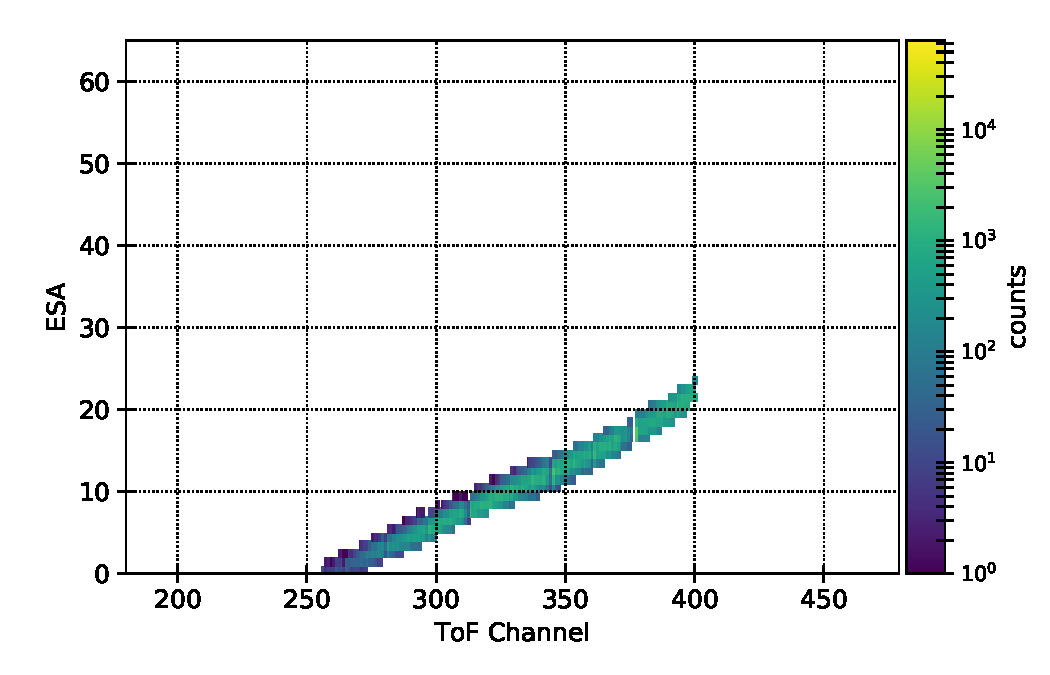
\includegraphics[width=1\linewidth]{Figures/epq_He1.pdf}
	\centering
\end{subfigure}
\begin{subfigure}{.9\linewidth}
	\centering
	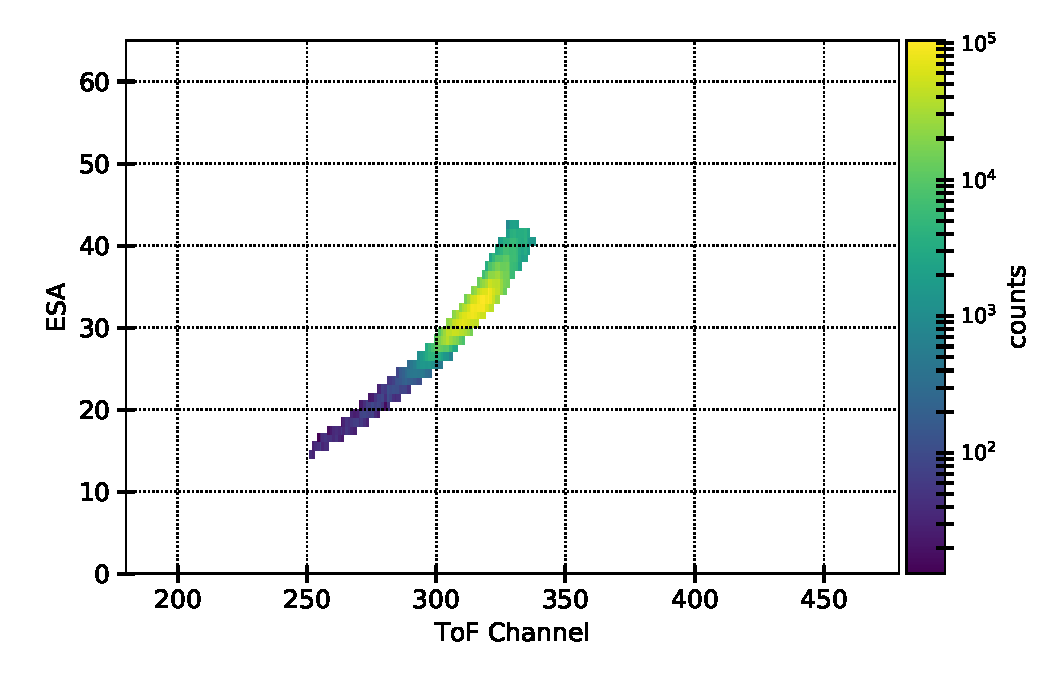
\includegraphics[width=1\linewidth]{Figures/epq_He2.pdf}
	\centering
\end{subfigure}
	\caption{$\mathrm{He^{+}}$ (above) and $\mathrm{He^{2+}}$ (below) selections that have been cut out from fig. \ref{fig:epq_rng0}.}
\label{fig:cutouts}
\end{figure} 
% Chapter Template

\chapter{Data Analysis and Methods} % Main chapter title

\label{Chapter:Data} 

%----------------------------------------------------------------------------------------

%----------------------------------------------------------------------------------------

Intro:\\
von den Rohdaten zur 3D VDF






\section{Coordinate Systems}
For orientation bla we need coordinate system bla...

%
\subsection{Ulysses trajectory, HG system}
\textbf{Todo: Hinweis auf Zeichnung und Kapitel vorne}\\
Trajectory data is used from \citet{ulysses-data-archive} where Ulysses position data on a daily basis is available. The trajectory data is given based on different coordinates, including the heliographic coordinate system in the B1950.0 epoch.
\\ \\
Heliographic Coordinate System:\\
The heliographic (HG) coordinate system is a Cartesian Sun-centered system with the Sun's equatorial plane as a reference plane. Its X-axis is directed along the line of ascending node, which is the intersection line of the ecliptic and the solar equatorial plane. While the solar equatorial plane has an inclination of $i_\odot 7.25 ^\circ$ against the ecliptic \citep{fraenz_harper} the line of ascending node is at a longitude of $\Omega_\odot \approx 75^\circ$ relative to the First Point of Aries in 1950 \citep{nasa-earth-coord}. The Z-axis of the HG coordinate system is directed along the Sun's spin axis (northward) and the Y-axis completes the right-handed system. \\
In HG spherical coordinates the longitude $\varphi_{HG}$ is defined to be $0^\circ$ for directions along the X-axis and increases towards the Y-axis. The latitude $\vartheta_{HG}$ is $0^\circ$ for direction within the solar equatorial plane and $+90^\circ$ for northward directions.\\ \\
%
%
When working with the Ulysses trajectory data it was found that these data were given in spherical coordinates for which the $\varphi_{HG} = 0^\circ$ direction was towards $\sim -105 ^\circ$ longitude relative to the First Point of Aries. This means that the Ulysses trajectory coordinate system is shifted $180^\circ$ around the solar spin axis against the classical definition (s.a.).\\
In fig. \ref{fig:traj} Ulysses' spherical HG coordinates as well its distance from the Sun are given over the time of nearly the complete mission.


\begin{figure}[h]
	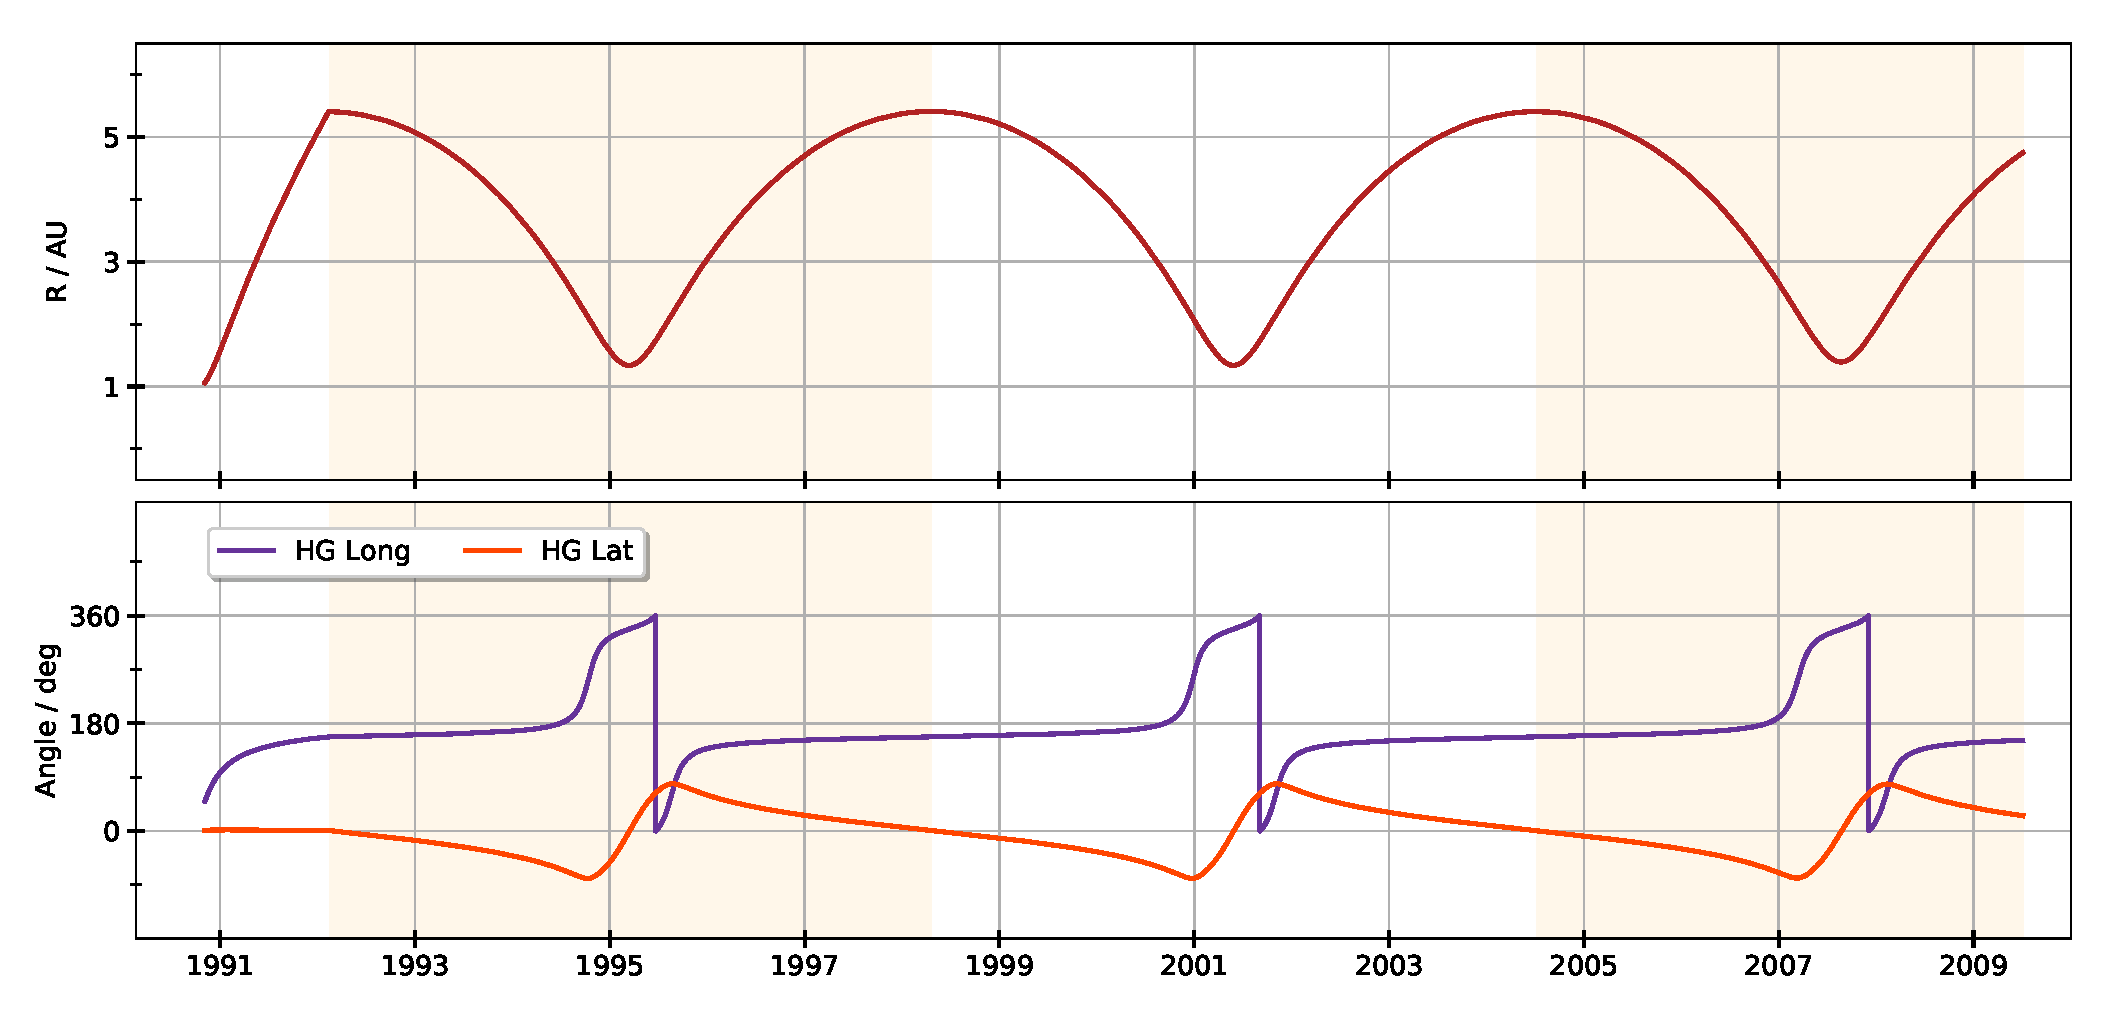
\includegraphics[width=1\textwidth]{Figures/HG_coord.pdf}
	\centering
	\caption{Ulysses trajectory data from November 1990 to June 2009 based on the data from the \citet{ulysses-data-archive}. Color shaded are the three orbits of the mission. \textbf{Above:} Shown is Ulysses' radial distance R from the Sun. Perihelion and aphelion of Ulysses' elliptical orbit can clearly be seen as the nearest/farthest distance of $1.3\,\mathrm{AU}$ and $5.4\,\mathrm{AU}$. Ulysses passes each of these points every 6.2 years and three times in total over the duration of the mission. \textbf{Below:} Shown are Ulysses' heliographic (HG) longitude and latitude. Note, that the longitude is shifted around $180^\circ$ with respect to the classical definition (s. text for details). A clear periodicity over Ulysses' three orbits can be seen. Maximum and minimum latitude are $\sim \pm 80^\circ$. These points are highest above the poles of the sun and are reached a few weeks before and after Ulysses' pass through the perihelion.}
	\label{fig:traj}
\end{figure}

\subsection{RTN Coordinate System}
Umrechnung von HG in RTN?
\\ \\
TODO:
The orbit itself is described in heliographic coordinates, so a cs that is constant (stable?) with respect to the sun. For describing positions and velocities in the frame of the spacecraft (e.g. AA) we need another cs...

\begin{figure}[h]
	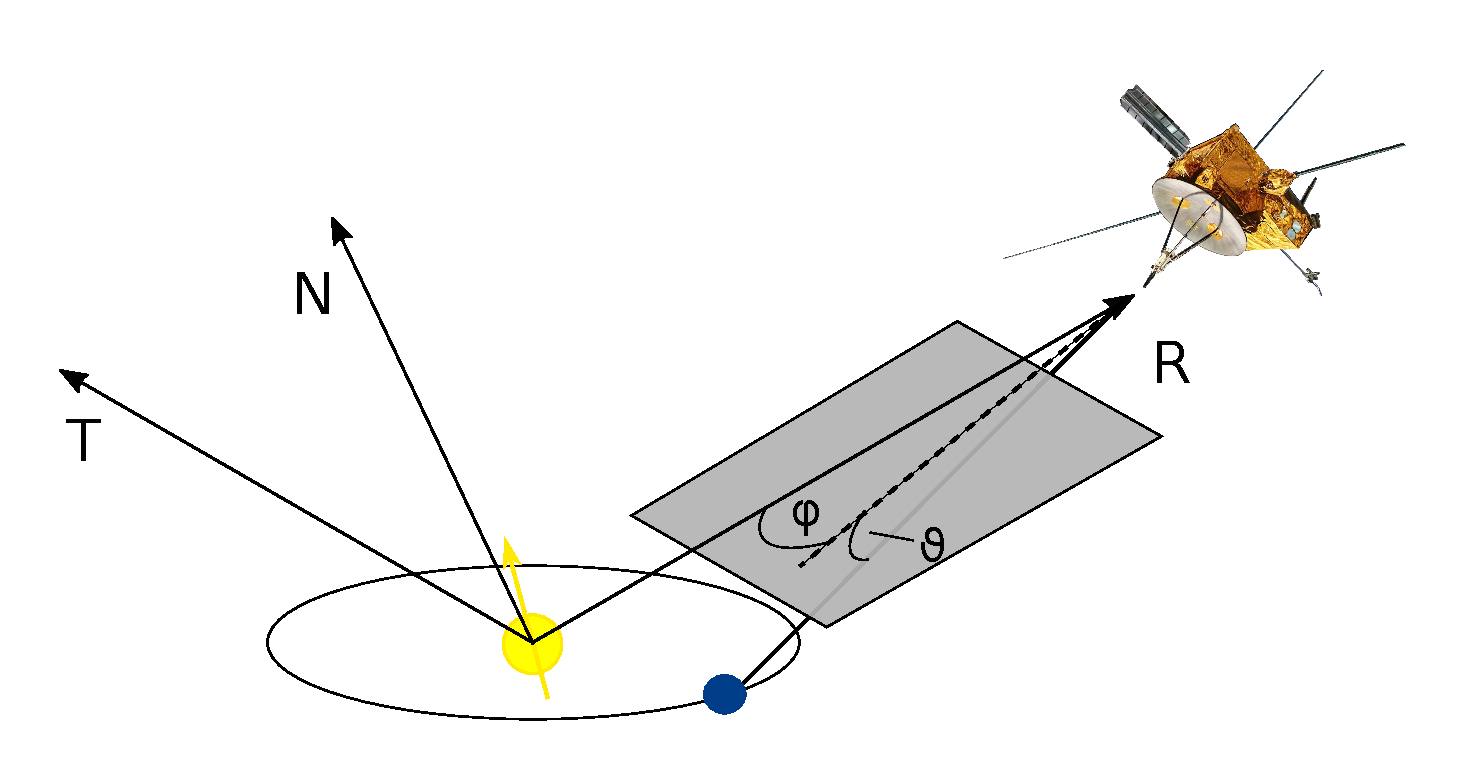
\includegraphics[width=1\textwidth]{Figures/RTN_AA_angles.pdf}
	\centering
	\caption{Graphical representation of the RTN coordinate system (not to scale). Shown are the Sun (yellow), the Earth (blue) and the Ulysses spacecraft at a non-specific position on its orbit. $\vec{R}$ is defined as the unit vector along the line-of-sight Sun--Earth, $\vec{T}$ as the normalized cross product $\vec{\omega} x \vec{R}$ with $\vec{\omega}$ the angular velocity of the Sun (yellow vector). $\vec{N}$ completes the right-handed Cartesian system. Also shown is the definition of the aspect angle components $\varphi_{\mathrm{asp}}$ and $\vartheta_{\mathrm{asp}}$ as they are used in this work. The grey plane depicts the $\vec{R}$--$\vec{T}$ plane. $0 ^\circ < \varphi_{\mathrm{asp}} < 90^\circ$ and $-90 ^\circ < \vartheta_{\mathrm{asp}} < 0^\circ$ in the shown situation. \textbf{TODO: Zeichnung anpassen: Vektorpfeile, Indizes Winkel; Quelle Ulysses Dingsi}}
	\label{fig:rtn}
\end{figure}


For dealing with Ulysses' trajectory data it is useful to work with \textit{radial-tangential-normal} coordinates. The RTN coordinate system is defined relative to a moving object in the heliosphere -- in this case the spacecraft, Ulysses, and is centered at the sun. A graphical representation on the system can be found in fig. \ref{fig:rtn}. The unit vectors are $\vec{R}$, $\vec{T}$ and $\vec{N}$, where $\vec{R}$ points radially outward from the sun to the current position of the spacecraft. $\vec{T}$ is defined as the normalized cross product of the Sun's angular velocity $\vec{\omega}$ and $\vec{R}$. $\vec{N}$ completes the right-handed Cartesian coordinate system. Consequently, the RTN system is not defined for a spacecraft's position right above one of the Sun's poles as the cross product $\vec{\omega} x \vec{R}$ is zero here. Nevertheless we do not have to worry about this fact as not even Ulysses crosses the poles directly (todo: Verweis?).




%
%
%
\section{Collimator/Detector model}
\begin{figure}
	\centering
	\begin{subfigure}{.5\textwidth}
		\centering
		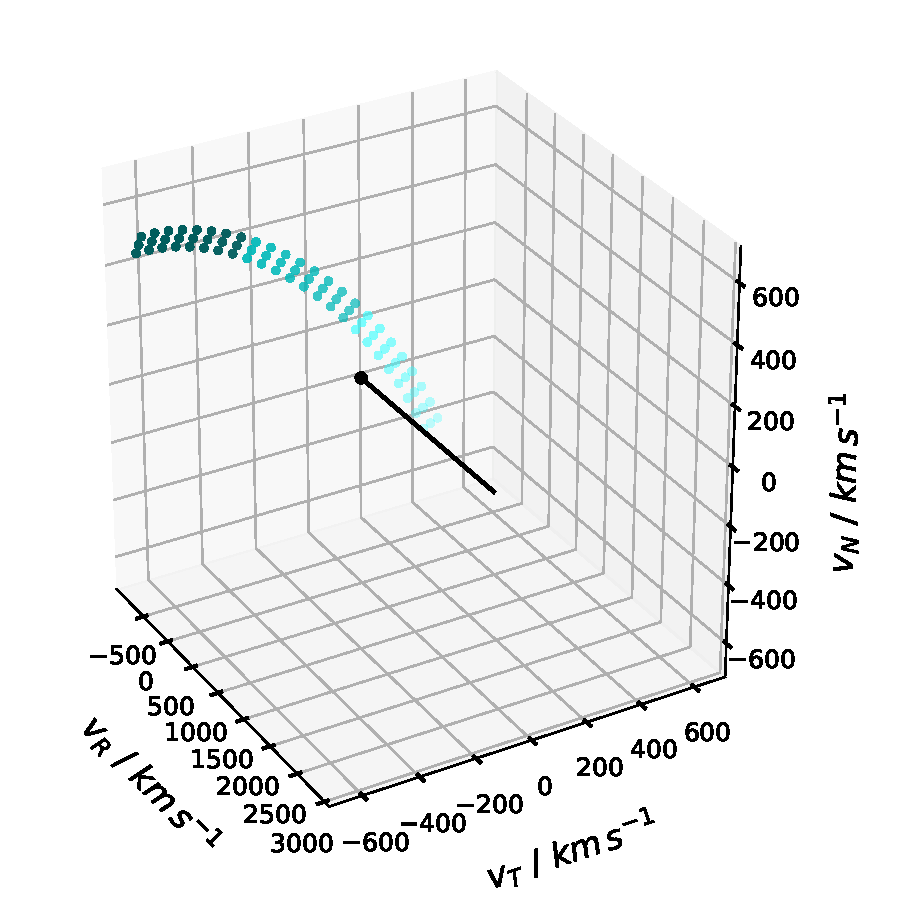
\includegraphics[width=1\linewidth]{Figures/col_single_new.pdf}
		\caption{A subfigure}
		\label{fig:sub1}
	\end{subfigure}%
	\begin{subfigure}{.5\textwidth}
		\centering
		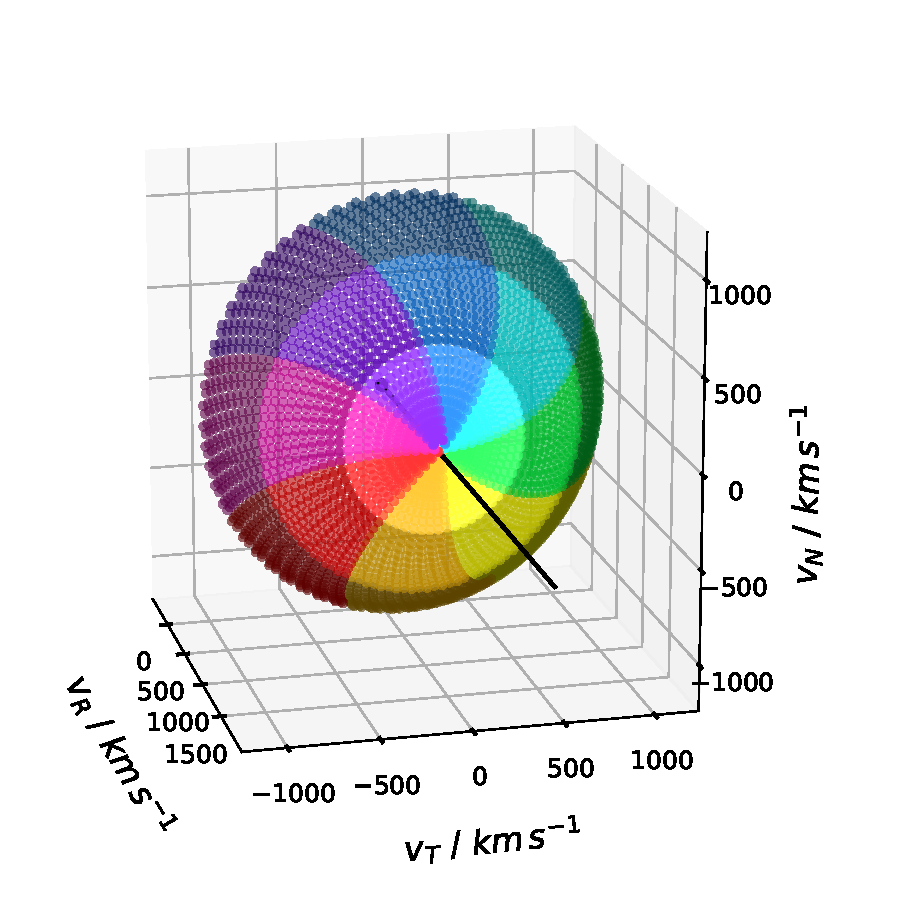
\includegraphics[width=1\linewidth]{Figures/col_vspace_normal.pdf}
		\caption{A subfigure}
		\label{fig:sub2}
	\end{subfigure}
	\caption{A figure with two subfigures}
	\label{fig:test}
\end{figure}
\begin{figure}[h]
	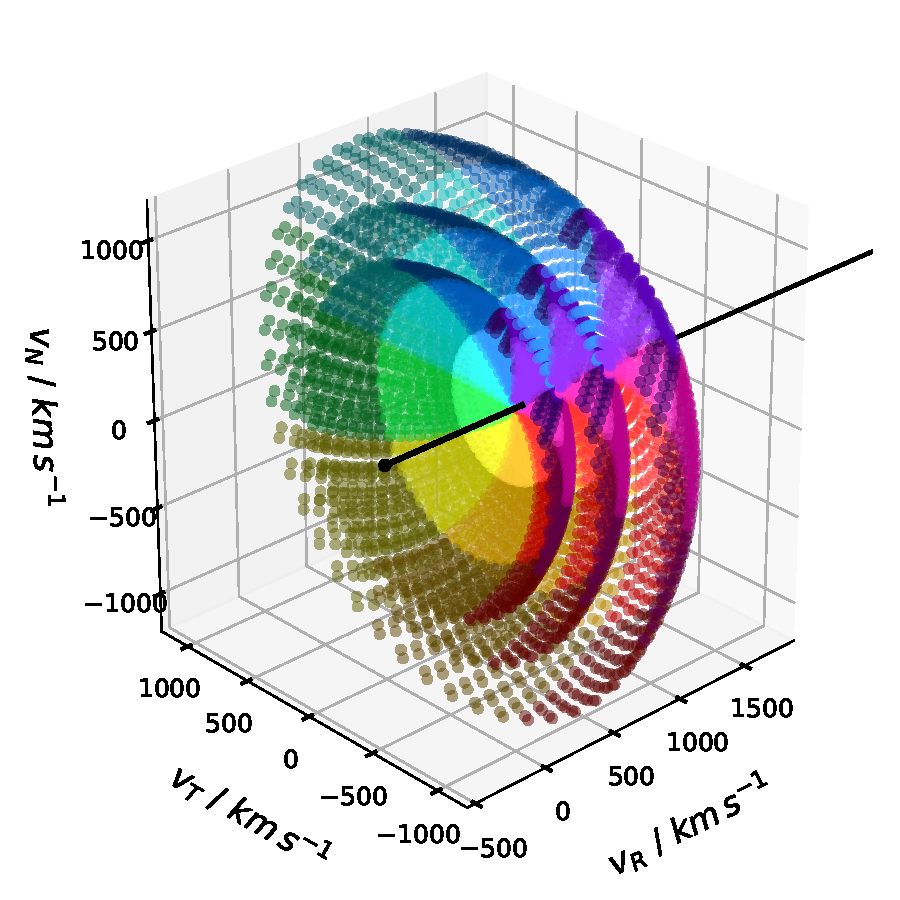
\includegraphics[width=0.5\textwidth]{Figures/col_shells.pdf}
	\centering
	\caption{TODO}
	\label{TODO}
\end{figure}
Schreiben, dass das eigentlich von ACE/Lars kommt

\subsubsection{Motivation}
Kollimatormodell -- warum eigentlich -- wie umgesetzt?\\ \\
Das Ziel ist, einem gemessenen Teilchen einen v-Vektor zuzuordnen. Eine Sek-Det-Kombi ist aber nicht eindeutig. Ihre Bedeutung hängt davon ab, wohin das Instrument guckt (FoV), von der Eigengeschwindigkeit des SC und davon, wie das SC gerade gedreht ist. Zusätzlich hat der Kollimator eine komplizierte Geometrie, sodass eine analytische Lösung schwierig ist: Also numerische Lösung. \\
Was macht das Modell? -- Ich will das FoV zu jedem Zeitpunkt bestimmen. Ich nehme dafür einzelne Messpunkte auf der originalen Geometrie. Dann gebe ich noch ins Modell, wie das gerade ausgerichtet ist.\\
Berechnet anhand des AA, wohin Sun trigger schaut, wenn getriggert wird und rotiert coll. an entsprechende Position für Sek 0. Ordnet entsorechend andere Sektoren an.
Simuliert FoV durch Punkteraster \\
\subsection{Construction} \label{subsec:construction}
For reconstructing the velocity space that SWICS measures we need to know about the directions of incident particles that can enter the instrument.
\\ \\
The original geometry of the SWICS entrance system, in particular the collimator, was read out from a technical drawing \textbf{\textbf{(TODO: Quelle?!})}
Can be described as:
Width: Cutting out a hollow piece of 90 deg longitude (\textbf{todo: latitude? 4 grad?}) from a sphere (\textbf{of r ca. 26 cm ??}) at .. deg polar latitude. The piece is not flat but curved and has a height of ca. 5 cm. This geometry leads to two deflection plates that are curved but have a constant distance of ca. 3.7 cm over a relatively large area which is necessary to provide a constant voltage for the EpQ filtering (s. \ref{sec:EpQ}). Resulting opening angles of the collimator are $69^\circ$ in width and $4^\circ$ in height. \textbf{Todo: Zeichnung/Abbildung?}\\
The instrument is mounted with one of the narrow side edges parallel to Ulysses' spin axis. When we define this edge to lie on the x-axis of a three dimensional Cartesian coordinate system, the collimator geometry can be reconstructed by revolving this edge for $90^\circ$ around a straight line that lies in the xy-plane with an angle of $56^\circ$ relative to the x-axis. \textbf{Todo: Zeichnung/Abbildung!} Every third of these $90^\circ$ is reserved as the opening angle for each of the three detector elements, that are described in \textbf{Todo}.  \\
The detector's field of view is the solid angle over which the detector is sensitive to incoming particles.
It can be represented by a set of outward directed normal vectors on the opening plane of the detector. In our model, we have a variable number of those equidistant vectors both along the width and the height of the detector opening. The real continuous field of view is modelled better with an increasing number of normal vectors that cover the opening. Each of these normalized vectors $\mathrm{\mathbf{f_i}}$ has a unique direction $\mathrm{\mathbf{f_i} = \begin{bmatrix}f_{x,i}\,f_{y,i}\,f_{z,i}\end{bmatrix}}'$ in position space. An example... \textbf{(TODO: Plot)}
\\
With a spin of the Ulysses spacecraft the fixedly mounted SWICS instrument is revolves as well around the spacecraft spin axis. Consequently, the field of view is revolved around the x-axis in fig todo. One revolution of SWICS is divided up into eight sectors per $45^\circ$ each (todo: Verweis auf Instrumentenkapitel oder Erklärung). As the spacecraft is spinning continuously, also the real field of view changes its rotation angle continuously.
For our virtual detector we model this by rotating the field of view gradually over n steps through every sector.\\
The integrated field of view over one spin then comprises TODO single vectors $\mathrm{\mathbf{f_i}}$ which are directed symmetrically around the spin axis (s. Abbildung TODO)). In fig. Todo is shown the FoV of todo , you can see a shell with radius 1 bla...
\subsubsection{From FoV to Vspace}
The detector's velocity acceptance can be calculated by combining the directional information from the field of view and the value of absolute velocity from the current EpQ step. 
\\
A particle can only enter the detector when its absolute velocity is within the acceptance of the current EpQ step and when its inverted direction is within the detectors field of view. For a given acceptance velocity $v_i$ and a single field of view vector $\mathrm{\mathbf{f_i} = \begin{bmatrix}f_{x,i}\,f_{y,i}\,f_{z,i}\end{bmatrix}}'$ the accepted velocity is
\begin{align}
\mathbf{v_i} = \begin{bmatrix}v_{R,i}\\v_{T,i}\\v_{N,i}\end{bmatrix} = - \begin{bmatrix}f_{x,i}\\f_{y,i}\\f_{z,i}\end{bmatrix} \cdot v_i.
\label{eq:fov}
\end{align}
With consideration of the integrated field of view over one spacecraft spin (s. ), the acceptance velocity consists of the combination n\_todo discrete velocities which form a shell with radius $v_i$ in velocity space. (s. fig. TODO for v\_todo)
\\ \\
HISCALE: "The experiment provides information about the spatial origin of events by treating each spin as eight sectors of approximately equal duration." \\ \\ \\


.
\\ \\
The central velocity for an ion of charge $q$ and mass $m$ for an energy-per-charge step $EpQ$ (in $keV/e$) is
\begin{align*}
\frac{v_c}{km \, s^{-1}} = \sqrt{\frac{2 \cdot EpQ \cdot 1.60217646\cdot10^{-19}\cdot |q|}{m \cdot 1.66053886 \cdot 10^{-27}} }
\end{align*}
with $m = 4 u$ and $|q| = 1$ for $\mathrm{He^{+}}$.\\
To represent the uncertainty in EpQ measurement, we take into account the relative uncertainty $\Delta \frac{E}{q}/\frac{E}{q} = \pm 5\%$ and translate it into an uncertainty $\Delta v / v = \frac{1}{2} \left( \Delta \frac{E}{q}/\frac{E}{q}\right) = \pm 2.5\%$ in accepted velocity. For every EpQ step we can now choose a number of $i_{epq}$ single velocities that are distributed evenly in the interval $\left[ v_c - \Delta v / v, v_c + \Delta v / v \right]$. The total number of accepted velocities $v$ is then $64 \cdot i_{epq}$.
\\
Different absolute velocities $v$ appear as distinct shells of radius $v$ in velocity space.
Ein Beispiel, der Übersichtlichkeit halber nur 3 Schalen, ist in bla gezeigt.
\\
With combining all $64 \cdot i_{epq}$ shells we obtain a dense three dimensional pattern of accepted velocities that simulate the real continuous velocity acceptance volume of the spinning detector.
\\ \\
When we measure a PHA word with a distinct SEC, DET and EPQ information, we can now determine its three dimensional velocity with our virtual detector. Of course, the resolution is limited as sector and detector areas are finite as well as the uncertainty $\Delta \frac{E}{q}/\frac{E}{q}$. By spreading the count over the entirety of velocity acceptances in the volume of the SEC DET EPQ combination, we take into account every velocity that could have led to this distinct PHA word.
\\ \\


.\\ \\ \\
Später schreiben, was für n verwendet wurden
\subsection{Eigen-velocity}
For the considerations in the previous section we assumed a detector on a spacecraft that is fixed in space. Obviously this is not the case for the Ulysses spacecraft (s. sec. TODO) which moves on its elliptical orbit around the Sun. \\
For determining the spacecraft's velocity we make use of the daily given trajectory data from sec. TODO. For every time stamp $t_i$ we calculate the spacecraft's instantaneous velocity by forming the differential quotient 
\begin{align*}
v_i = \frac{ \begin{bmatrix}v_{R,i+1}\\v_{T,i+1}\\v_{N,i+1}\end{bmatrix}_i  - \begin{bmatrix}v_{R,i}\\v_{T,i}\\v_{N,i}\end{bmatrix}_i} {t_{i+1} - t_i}
\end{align*}
with $t_{i+1}$ being the next time stamp, which is normally $t_i + 1\,\mathrm{d}$. Note, that the spacecrafts position at $t_{i+1}$ has to be considered in the RTN coordinate system that relates to the spacecraft's position at $t_i$. The resulting velocities in RTN coordinates are shown in fig. todo.
\\
--Bewertung Größenordnung--
\\
To correct the measured velocities for the spacecraft's eigen-velocity, we simply add the resulting velocity components to the velocity acceptance. Thus, for every time stamp the shells (s. fig todo) are shifted a bit in velocity space based on the respective eigen-velocity.


\subsection{Orientation of the Detector}
Until now we have assumed that Ulysses' spin axis is aligned with the R-axis of the coordinate system, i.e. that the spin axis points directly to the Sun. In fact, this is not the case in general. Due to telemetry reasons, Ulysses' high gain antenna has to be oriented directly towards Earth (todo: Vergleich mit ACE, warum?). As Ulysses' spin axis is aligned with the electrical axis of the antenna \citep{wenzel_ulysses}, has an offset towards the line of sight spacecraft-Sun. This offset is called \textit{aspect angle} and is a permanently changing quantity as a function of Ulysses' position and the position of the Earth. As a varying aspect angle results in SWICS covering different parts of velocity space it is essential to consider this quantity in detail.
%
%
\subsubsection{Calculation of the Aspect Angle}
\begin{figure}[h]
	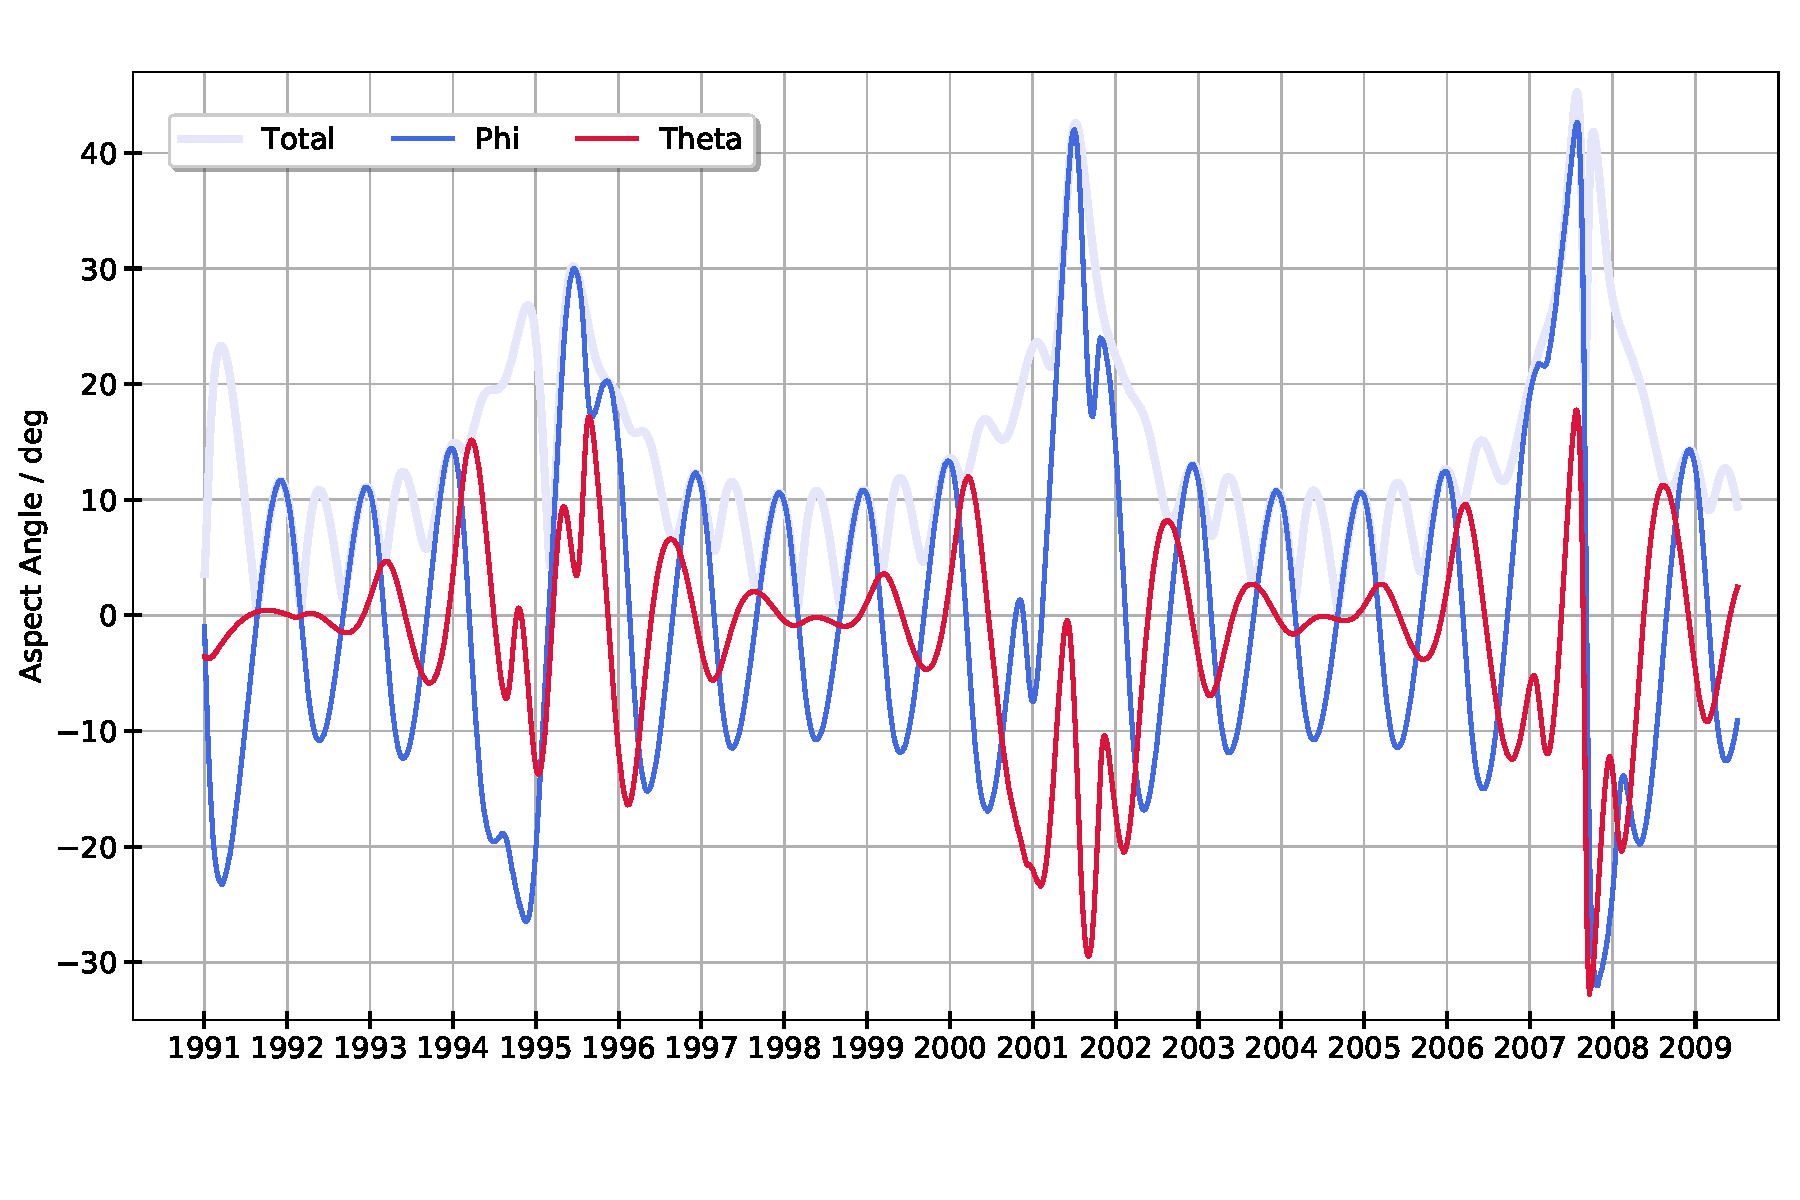
\includegraphics[width=1\textwidth]{Figures/aa_new.pdf}
	\centering
	\caption{The evolution of Ulysses' aspect angle components $\varphi_{\mathrm{asp}}$ and $\vartheta_{\mathrm{asp}}$ from 1991 to the end of the mission are shown. The aspect angle is the angle between the line-of-sight Ulysses--Sun and the orientation of Ulysses' spin axis. A constantly changing aspect angle results from the fact that the spacecraft's antenna, that is nearly parallel with the spin-axis, has to point towards Earth all the time. Particularly large aspect angles occur during the three fast latitude scans around 1995, 2001 and 2007. Here, Ulysses' distance to Sun and Earth is at a minimum. \textbf{Also shown is the... (todo: raus aus der Zeichnung?)} }
	\label{fig:aa}
\end{figure}
The aspect angle is measured from the line-of-sight Ulysses--Sun (that is $\vec{R}$) to the line-of-sight Ulysses--Earth. To describe this angle uniquely for any moment, we need two spherical coordinates $\varphi_{\mathrm{asp}}$ and $\vartheta_{\mathrm{asp}}$ based on the RTN system. As shown in fig. \ref{fig:aa}, $\varphi_{\mathrm{asp}}$ is measured in the $\vec{R}$--$\vec{T}$ plane between $-\vec{R}$ and the projection of the line-of-sight from Ulysses to the Earth into this plane. $\varphi_{\mathrm{asp}}$  is $0^\circ$ for directions along $-\vec{R}$, that is the line-of-sight from Ulysses to the Sun and increases to positive values towards $-\vec{T}$. $\vartheta_{\mathrm{asp}}$ is the angle between the projection of the line-of-sight from Ulysses to the Earth into the $\vec{R}$--$\vec{T}$ plane and the line-of-sight itself. It is defined as $0^\circ$ for directions that lie within the $\vec{R}$--$\vec{T}$ plane and $+90^\circ$ for directions along $\vec{N}$.\\
(Todo: Lars fragen, ob die genaue Rechnung hier rein muss, Kladde S. 79)
For the calculation of the aspect angle we used the Ulysses trajectory data (Verweis ... TODO) and Earth trajectory data in heliographic coordinates on a daily basis from \citet{nasa-earth-coord} and converted both to RTN coordinates. In fig. \ref{fig:aa} both components $\varphi_{\mathrm{asp}}$ and $\vartheta_{\mathrm{asp}}$ as well as the \textit{flat} aspect angle $\alpha$ with  $\alpha = \arccos(\cos{\varphi_{\mathrm{asp}}}) + \arccos(\cos{\vartheta_{\mathrm{asp}}}) -1$ are shown over the time of the mission. $\varphi_{\mathrm{asp}}$ varies in the range from $\sim - 25^\circ$ to $\sim 42^\circ$ and $\vartheta_{\mathrm{asp}}$ in a range from $\sim - 30^\circ$ to $\sim 17^\circ$. Large angles occur especially around the three fast latitude scans, i.e. when Ulysses is at its perihelion and has the smallest distance to Sun and Earth.\\
(Todo? Beschreiben, dass ich $\alpha$ mit dem Datenprodukt SPE verglichen habe?)
\\ \\
\begin{figure}[h]
	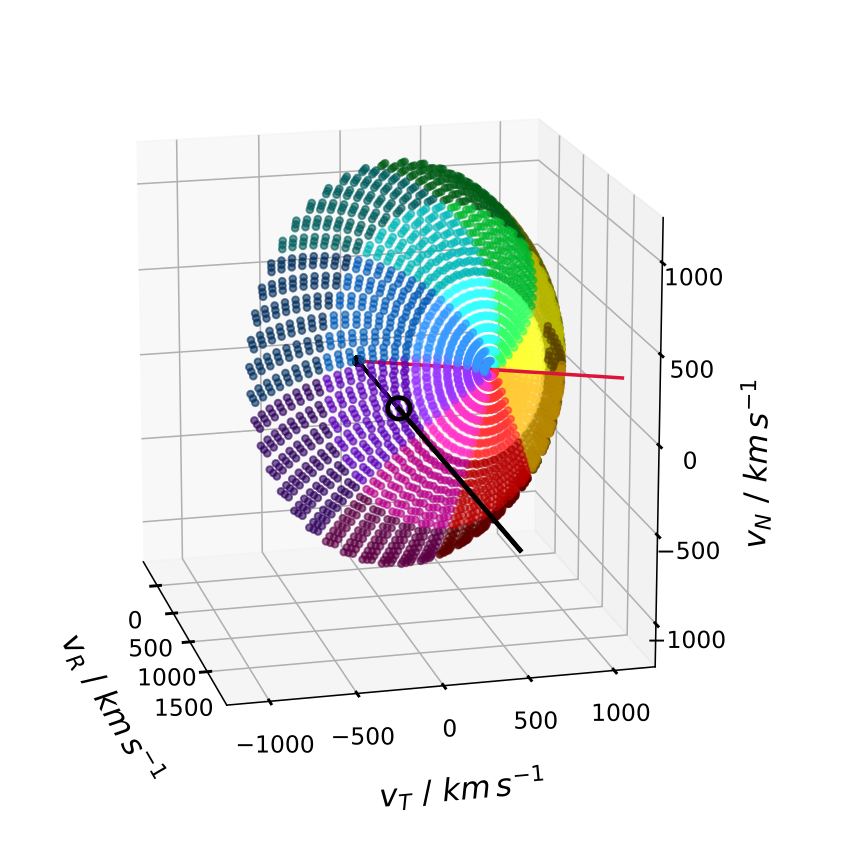
\includegraphics[width=0.5\textwidth]{Figures/col_aa_marker.png}
	\centering
	\caption{todo}
	\label{fig:col_aa}
\end{figure}
steps asp Winkel

The variable aspect angle is incorporated into the analysis by rotating the field of view corresponding to $\varphi_{\mathrm{asp}}$ and $\vartheta_{\mathrm{asp}}$. This results in a likewise rotation of the velocity acceptance space. In fig. \ref{fig:col_aa} the acceptance velocity for a single absolute velocity $v = 600\,\mathrm{km\,s^{-1}}$ is shown for $\varphi_\mathrm{asp} = 25^\circ$ and $\vartheta_{\mathrm{asp}} = -10^\circ $. Note, that the orientation here seems to be mirrored against the convention that has been described before. This is due to the inversion when transitioning from the field of view to velocity acceptance, s. eq. \ref{eq:fov}.\\
When comparing fig todo with fig todo, where a situation with $\vartheta_{\mathrm{asp}} = \varphi_{\mathrm{asp}} = 0$ is shown, it becomes clear that especially larger aspect angles change the link between a distinct sector-detector element and a volume in velocity space. While with a zero aspect angle a radial velocity (along $\vec{R}$) would be detected right in the middle of the velocity shell and definitely in the innermost detector, this is not the case for the aspect angle in fig. todo. Here, an exclusively radial oriented velocity would be detected in a distinct sector in the central detector. (Andersrum bedeutet das, dass eine Sec-Det-Info nur zugeordnet werden kann, wenn die Ausrichtung des Detektors bekannt ist!)

\subsubsection{Probe}
For checking if the considerations made before are reasonable and if the virtual detector works in the right way, we want to have a look at data of which we believe to know the VDF. Appropriate test data is the solar wind itself as it is believed to flow radially outwards from the sun (Todo:Quelle). An ideal candidate within the solar wind is $\mathrm{He^{2+}}$ as the most abundant species (todo: Quelle). Thus, we can identify $\mathrm{He^{2+}}$ easily in fig Todo and are provided with good statistics. Unlike protons, which are even more abundant in the solar wind, $\mathrm{He^{2+}}$ most likely deposits energy above the detector's threshold in the SSD detector (s. chap Todo). This is because of its higher mass and the twice as high charge, which leads to a higher gain in energy by the post acceleration (todo:nochmal Verweis?). Only when a particle triggers an ESSD measurement (Triple Coincidence) we get a directional information about its velocity (Verweis todo). Protons are most often measured as Double Coincidences except for suprathermal protons, for which the assumption of radial stream must not hold true (Todo:Quelle). For selecting $\mathrm{He^{2+}}$ we proceed like described in chap. todo.
Wie viele PHAs sind das dann insgesamt und pro Jahr? Schreiben, dass das nicht so genau gemacht werden musste, weil keine VDF Analyse...
\\ \\
In a first step we look at periods of time in which both aspect angle components $\varphi_{\mathrm{asp}}$ and $\vartheta_{\mathrm{asp}}$ were small (Todo: genau?). For these nr\_todo PHA words we draw a histogram (??) of their sektor and detector information. The result can be seen in fig. todo. The histogram shows that mainly the innermost detector has counts. This is the expected behavior when we imagine the instrument on a spacecraft that points directly to the Sun. A radially streaming flow then hits the instrument's detector that is oriented sunwards. This does not change with the spin of the spacecraft. This result is also consistent with the detector model for $\varphi_{\mathrm{asp}} = \vartheta_{\mathrm{asp}} = 0$ which is shown in fig. todo. A radial stream can be represented here by the black line which cuts through the velocity shell in its center, the region of the innermost detector, bla. Irgendwie schöner schreiben...
(Due to the width... auf allen Sektoren?)
\\ \\
In a second step we take a look at a time period in which Ulysses had a substantial aspect angle. This is particularly the case for when Ulysses is near its perihelion, s. fig todo. We choose for the second orbit, i.e. days 1-90 (?) in 2001. For all $\mathrm{He^{2+}}$ PHA data from this time we again histogram sector and detector information, which is shown in fig. todo. Compared to fig. todo the maximum of counts is now shifted clearly towards a single sector (Nr.?) and the central detector. This is consistent with the virtual detector in fig. todo, where the aspect angle's quantity matches the one in the selected time period. With this orientation a radial stream from the Sun hits the instrument on its center detector and only while a particular moment (?!) of the spin/rotation (?!). Counts do not show up exclusively with this single sector-detector combination but slightly spread out over adjacent sector-detector elements. This is due to the fact that solar wind $\mathrm{He^{2+}}$ does not stream as an ideal beam but has a certain width (todo: Referenz).
\\ Verweis: Sektordetails im nächsten Kapitelchen

\begin{figure}[h]
	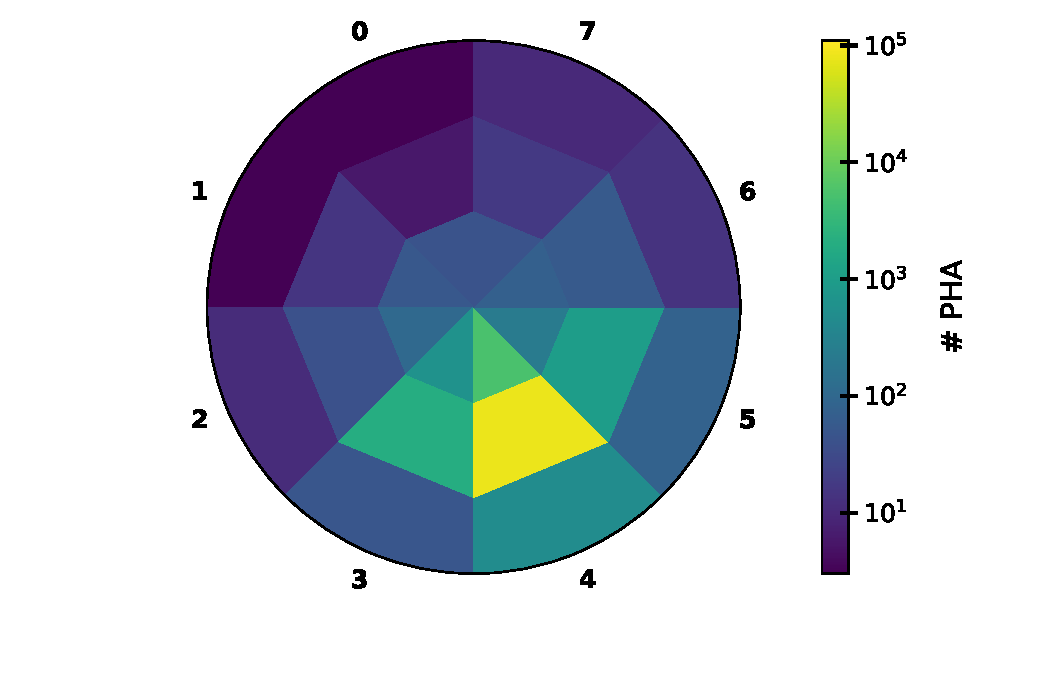
\includegraphics[width=0.5\textwidth]{Figures/hist_det_sec_aa_90days2001}
	\centering
	\caption{TODO}
	\label{TODO}
\end{figure}


\subsubsection{Sunpulse Trigger -- Rotation}
In the previous section hat man gesehen, dass sich die PHA Counts für einen großen AA auf den mittleren Detektor konzentrieren. In diesem Abschnitt soll geklärt werden, wovon es abhängt, in welchem Sektor der Schwerpunkt der Counts landet. 

As mentioned before (todo: ist es?), one SC spin is divided into 8 sectors, starting with sector 0 and ending with sector 7.
Every spin's start is defined newly by the \textit{spin reference pulse} of Ulysses \citep{hiscale}. 

This pulse is triggered by a combination of four sun sensors which detect when the Sun crosses a plane that is spanned by the spacecraft's spin axis and the spacecraft's x-axis, which is a particular axis perpendicular to the spin axis.
The spin reference pulse is not uniform over time as the position of the Sun relative to the spacecraft changes with varying aspect angle.\\
To extract correct directional information from a sector data product of an ion that has been detected by SWICS it is essential to know the relative orientation between SWICS' main axis and the x-axis on the spacecraft. In the virtual detector this is implemented as an angle against the line-of-sight spacecraft-sun by which the field of view is rotated around the spin axis.\\
From the \citet[][S.20-22]{swics_dpu} we know with \textit{normal orientation} the sun pulse occurs in the center of SWICS sector 4, which implies a $180^\circ$ offset between the line-of-sight spacecraft-sun and SWICS sector 0 (s. fig TODO). However, one can also read that it was possible to set a fine adjustment which would lead to an offset of the sun pulse from this center line up to $22.5^\circ$ \citet[][S.48]{swics_dpu}. Unfortunately, we do not know about the value that has been chosen.
\\
If we assumed a wrong angle, a particle beam coming from a fixed direction in a sun-fixed frame would be linked to a different direction. But this shift between true and supposedly measured direction is not constant over aspect angles. If we then measured over a longer time period with various aspect angles, we would measure the beam as blurred in velocity space.
\\
To make sure our model uses the right angle, we again choose $\mathrm{He^{2+}}$ as a test population of which we assume a beam-like behaviour streaming radially from the Sun. Also, we can only look at time periods when the aspect angles were large and the maximum of $\mathrm{He^{2+}}$ counts occurs in the central or outermost detector. Only here we can clearly discriminate between single sectors. When measured in the innermost detector the slightly widened distribution of $\mathrm{He^{2+}}$ would spread across all sectors as they are close together here (s. fig todo).
From fig Todo, where we histogrammed bla, we find that the overall idea of a sun pulse in sector 4 should be right when we believe the assumption that $\mathrm{He^{2+}}$ streams radially from the Sun. To check for a potential fine adjustment we search for tendencies of the maximum of counts sweeping to an adjacent sector.
\\
Zeigen: Für lange Zeiträume: $\mathrm{He^{2+}}$ kommt zentral. Für einzelne kurze: unterschiedlich.
Deshalb: grober Check von wegen Detektor geht gut. Für das Feintuning (180 Grad oder doch was anderes?) reichts aber nicht...
\\
Schemazeichnung SunPulser, dazu Problem irgendwie zeigen

\subsubsection{Übergang w}
Steps vsw
\\
With the considerations of eigen-velocity and orientation we can now use the virtual detector for displaying velocity distributions of $\mathrm{He^{+}}$ pickup ions. 

Mithilfe des virtuellen Detektors können jetzt geeignete (Triples) PHA Worte in dreidimensionale Geschwindigkeitskomponenten übersetzt werden (vorher: nur Betrag. Jetzt: Komponenten).
Erst mit diesen entfalteten Einzelkomponenten kann man den wichtigen Schritt gehen und in den Sonnenwindframe übergehen.
This is done for every PHA word (nein. jeder v-Akzeptanzpunkt in jeden getroffenen Sek-Det-Kombidings...) by subtracting the instantaneous solar wind speed in R-component from the ion's velocity in spacecraft frame: 
\begin{align*}
\mathbf{v_{i,sw}} = \begin{bmatrix}v_{R,i,sc}\\v_{T,i,sc}\\v_{N,i,sc}\end{bmatrix} - \begin{bmatrix}v_{sw}\\0\\0\end{bmatrix}
\end{align*}
In a last step every component of the resulting vector is divided the by solar wind speed:
\begin{align*}
\mathbf{w_{i,sw}} = \begin{bmatrix}v_{R,i,sw}\\v_{T,i,sw}\\v_{N,i,sw}\end{bmatrix} / \begin{bmatrix}v_{sw}\\v_{sw}\\v_{sw}\end{bmatrix}
\end{align*}
By this, the transition from velocity space in the spacecraft frame to solar wind independent w space in solar wind frame of reference is made.
%
%
%
\section{VDF}

%
\subsection{Velocity Space Coverage}
When analyzing $\mathrm{He^{+}}$ PUI w-spectra with Ulysses SWICS, several effects have to be considered that limit the observable part of w-space. The most obvious restriction results from the fixed geometry of the collimator (s. sec. \ref{subsec:construction})) which allows to observe only a dome-shaped part of the w-space when considering the spin of the spacecraft and varying EpQ steps. (However, this dome is not fixed in w-space for different orientations of the spacecraft.
While the ever changing aspect angle of Ulysses introduces a complex subject to directional data analysis it also enlarges the integrated coverage of velocity space over time.)\\
Furthermore, we have to deal with a limitation of the coverage in $w_R$-direction particularly for $\mathrm{He^{+}}$ triple coincidences. The observable EpQ range for $\mathrm{He^{+}}$ is limited to TODO to TODO, which corresponds to steps todo to todo. While A is the instrument's highest possible EpQ value, B is the lowest value for which $\mathrm{He^{+}}$ still has enough energy to overcome the energy threshold of the SSD and thus can trigger a valid energy measurement. 
The w-range that is consequently covered is highly dependent on the prevalent solar wind speed. For $v_{sw} = 700 \,\mathrm{km/s}$ the absolute w in a spacecraft frame is limited to TODO. For slow solar wind at $v_{sw} = 300 \,\mathrm{km/s}$ todo... . 
That means that we are limited to time periods with fast solar wind as we do not expect to measure the bulk of $\mathrm{He^{+}}$ PUI at w größer als... TODO. In fig. TODO an exemplary w-space coverage for vsw = Todo and no aspect angle is sketched.
\\ \\
Evtl. woanders hin und irgendwie besser schreiben: \\
In fig. \ref{fig:vsw_years} a histogram for occurring solar wind speeds is shown -- limited to times in which $\mathrm{He^{+}}$ triple coincidences were measured. Measured with SWOOPS. The number on the right indicates the total number of $\mathrm{He^{+}}$ PHA triple coincidence data that was received for that year. One can see the overall variation of the solar wind speed (due to different latitude: slow/fast sw) and that the total number of received data decreases heavily towards years in which Ulysses approaches the orbit's aphelion. This is mainly an effect of pickup ion flux reduction that scales with $r^{-2}$ due to the expansion of the solar wind (Todo:Quelle?).
\begin{figure}[h]
	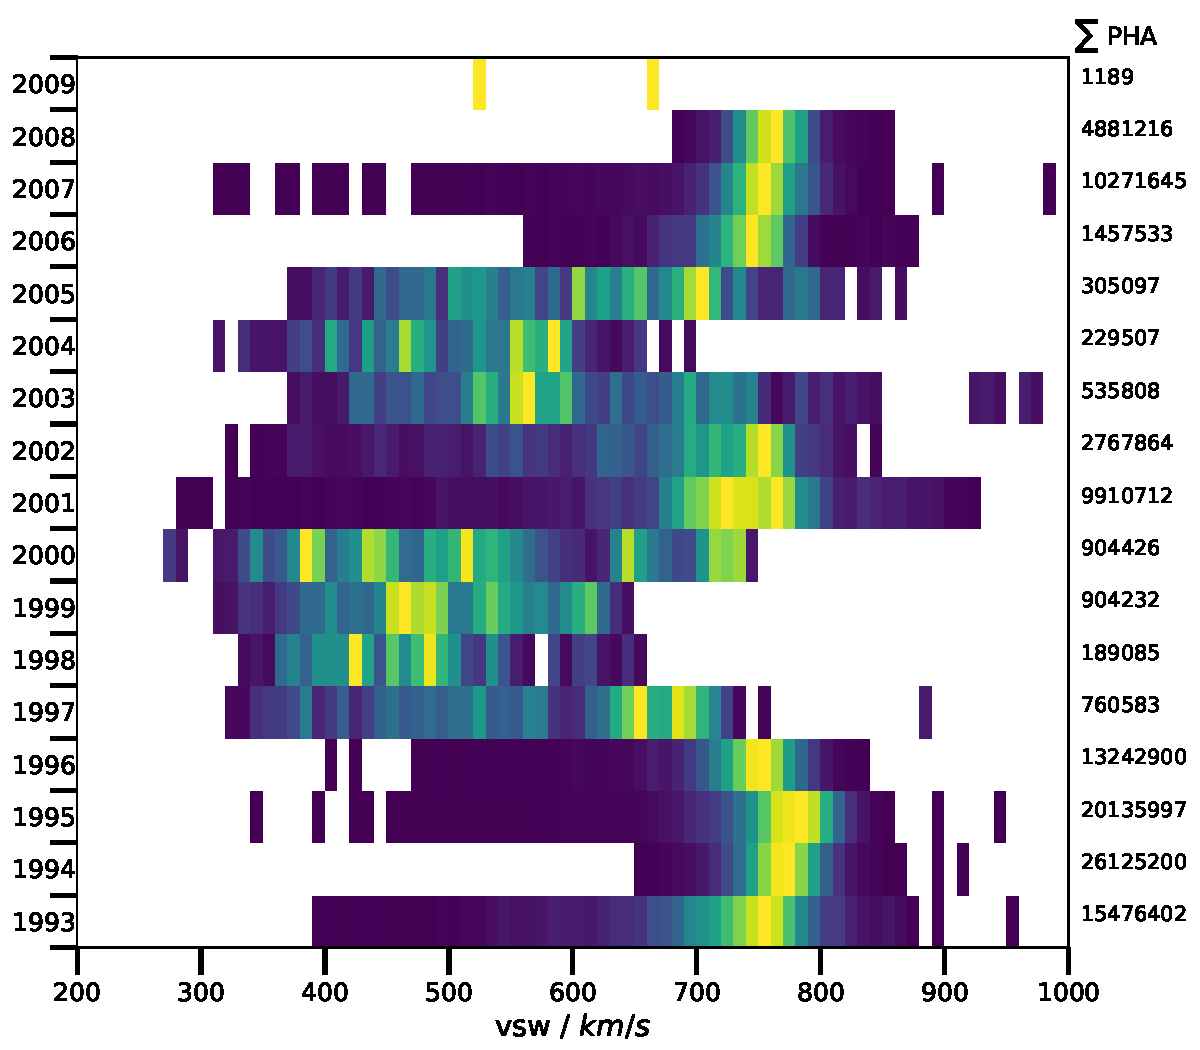
\includegraphics[width=0.9\textwidth]{Figures/vsw_all_years_brw.pdf}
	\centering
	\caption{TODO... u.a.: norm; pad links neu}
	\label{fig:vsw_years}
\end{figure}


%
\subsection{Phase Space Normalisation}
We are now able to combine the information about sector, detector and EpQ step from the selected $\mathrm{He^{+}}$ PHA triple coincidences with the information about how the spacecraft was moving and which direction it was facing at the time of the measurement.
Counts that we have collected over a certain time period can be mapped into three dimensional w-space by this. However, for deriving physical quantities from these, a transition from counts to phase space density has to be made.\\
Firstly, we consider a single spin of the spacecraft, which normally corresponds to one EpQ step of SWICS.
Counts $N_{jk}$ that have been measured in a phase space volume that has been covered by a sector-detector element $j$ during the EpQ deflection step $k$ can be connected to the average phase space density $\delta_{jk}$ in this volume by an integration over the three dimensional velocity space:


\begin{align*}
N_{jk} &= \iiint\displaylimits_{v_{\varphi j}v_{\vartheta j}v_{R k}} \rho_{jk}	V_k	\,\,	d^3v,
\end{align*}
where $V_k = G \, \tau \, v_k$ is the spatial volume of the measurement with the geometrical factor $G = 0.0225 \,\mathrm{cm^2}$ (TODO: Quelle. Bei gloeckler steht das nicht?), $\tau = 12/8\,\mathrm{s} = 1.5\,\mathrm{s}$, the time of the measurement in a single sector and $v_k$ the central velocity for $\mathrm{He^{+}}$ in the EpQ step $k$ (Todo: Plot, Formel? Und dann Verweis nach vorne).
With the opening angles of a single sector-detector element of $4^\circ$ in width and $69^\circ /3 = 23^\circ$ in length and the height of this element $\Delta v_k$ we can write
\begin{align*}
%&= \iiint\displaylimits_{v_{\varphi i}v_{\vartheta j}v_{R k}} \rho_{ijk} \,	G \, v_k \, \tau	\,\,	d^3v \\
N_{jk} &= v^2_k \left(\frac{\pi^2}{180^2}\cdot4 \cdot 23\right) \, \Delta v_k \, \rho_{jk} \,	G \, v_k \, \tau.
\end{align*}
$\Delta v_k$ is determined by the uncertainty in EpQ measurement. It has been found to be $\Delta v_k = 0.025 \, v_k$ in sec. todo:chaptr FoV to vspace, which gives us
\begin{align*}
N_{jk} &= v^4_k \left(\frac{\pi^2}{180^2}\cdot4 \cdot 23\right) \, 0.025\, \rho_{jk} \, G  \, \tau.
\end{align*}
This we can rewrite with the phase space volume $V_{k}$ as 
\begin{align*}
\rho_{jk} &= \frac{N_{jk}}{V_{k}}.
\end{align*}
Notice, that $V_{k}$ is only dependent on the EpQ step $k$, as the sector-detector elements span the same (absolute) phase space volume for one EpQ step.\\
When we want to measure more than one spin, it has to be considered, that the probability to detect an ion is dependent on the EpQ step. This behaviour can be described by the detection efficiency.
\\ \\
The detection efficiency can be considered in phase space normalisation by weighting the spanned phase space volume for every sector detector element with the efficiency of the respective EpQ step: 
\begin{align*}
\rho_{jk} &= \frac{N_{jk}}{V_{k}\cdot eff_k}.
\end{align*}
As the instrument covers different phase space volumes with varying aspect angle, changing parts of phase space volume are covered.
However, we are actually interested in the average phase space density at a distinct volume element in phase space. This we get by dividing the counts in the volume element $v_i$ by the measured volume, both integrated over time and this volume. This means that we consider the time in which we we could have measured blaaaa.
\begin{align*}
\rho_{v_a} = \frac{\iint\displaylimits_{t\,v_a} N \, dv dt}{\iint\displaylimits_{t\,v_a} V\,eff\,dv dt}
\end{align*}




%.
%\\ \\ \\
%Mittlere Phasenraumdichte in einem Bin, in den zwei Instrumentenbins A und B reingehen:
%(differential PSD)
%\begin{align}
%\bar{\rho} = \frac{N_A + N_B}{\frac{N_A}{N_{A,ges}} V_A + \frac{N_B}{N_{B,ges}} V_B }
%\end{align}
%Dabei ist $N_i$ die Anzahl der Hits, die im Messbin gelandet sind und $N_{i,ges}$ die gesamte Anzahl an Bins. Hits heißt GEsamtcounts durch Detektoranzahl. Eigentlich gebe ich statt $N_i$ $N_i \cdot Detektoranzahl$ rein, aber das kürzt sich ja raus.\\ \\
%Effizienz und Sektorgewichte dazu:\\
%Allg.:
%\begin{align*}
%\rho = \frac{N \cdot brw}{V \cdot Eff}
%\end{align*}
%Und dann
%\begin{align}
%\bar{\rho} = \frac{N_A + N_B}{\frac{N_A}{N_{A,ges}} \frac{V_A \cdot eff_A}{brw_A} + \frac{N_B}{N_{B,ges}} \frac{V_B \cdot eff_B}{brw_B} }
%\end{align}









% Chapter Template

\chapter{Results} % Main chapter title
\label{chap:results}
%B-Feld. Von welchem Instrument? auch RTN-System. Genauso Winkel berechnet.
%1-min-Mittel (Gyroradius Zeit zeigen) und entsprechend EpQ-Steps den PHAs zugeordnet.
%
%
%
Here we present first results of the method that has been developed in Chapter \ref{chapter:data} for $\mathrm{He^{+}}$. For creating three-dimensional velocity spectra from $\mathrm{He^{+}}$ SWICS PHA data we synchronize the selected data (s. Ch. \ref{chapter:instrumentation}, $\mathrm{He^{+}}$ Triple Coincidences) with the spacecraft's aspect angle, its eigen-velocity and the present solar wind speed.
This gives us directionally resolved counts from the observed phase space volume.
\\ \\
An example for data from a measuring period of 50 days in 1993, limited to solar wind speeds from $760 \, \mathrm{km\,s^{-1}}$ to $780 \, \mathrm{km\,s^{-1}}$, is shown in Fig. \ref{fig:counts_50}. Here we histogrammed the counts by utilizing Cartesian $w_{\mathrm{sw,R}}$, $w_\mathrm{sw,T}$ and $w_\mathrm{sw,N}$ bins in solar wind frame. Shown are counts from a ``slice'' in the $w_\mathrm{sw,T} - w_\mathrm{sw,N}$ plane. Counts within the range $0.3 <= w_\mathrm{sw,R} < 0.5$ have been summarized for each $w_\mathrm{sw,T} - w_\mathrm{sw,N}$ bin. The orientation of this cut is sketched in Fig. \ref{fig:sketch_slice_R} for better understanding.
\begin{figure}[h]
	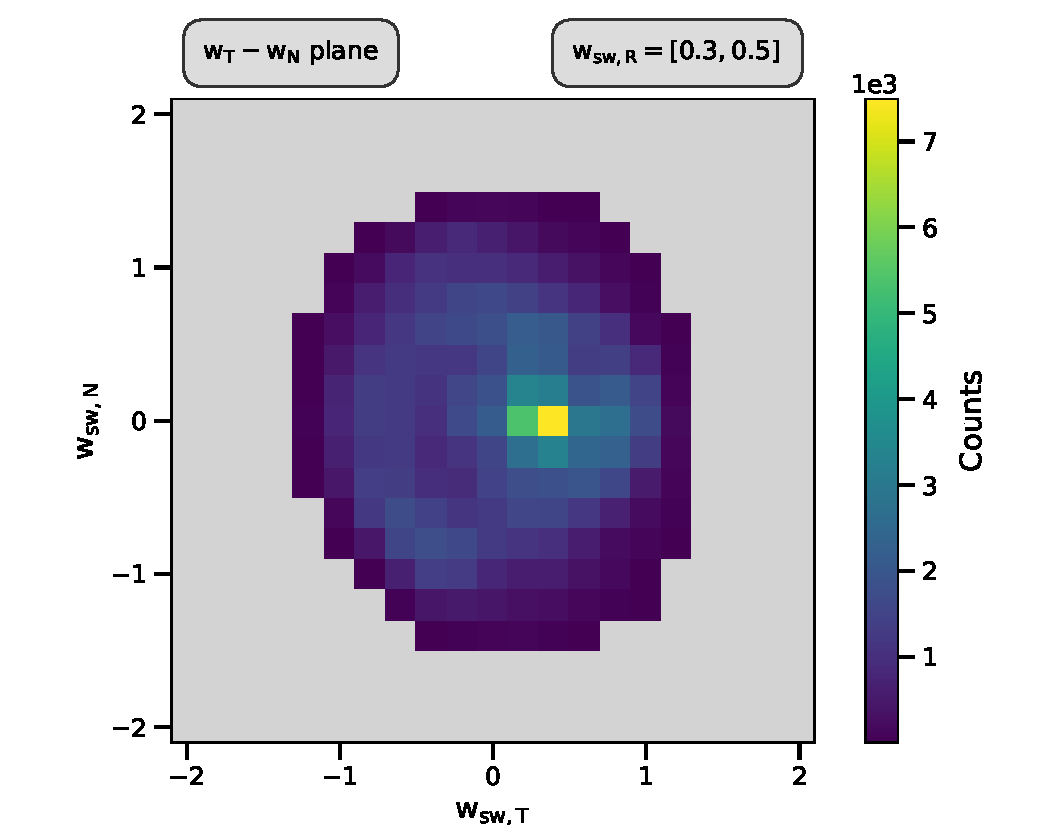
\includegraphics[width=.85\textwidth]{Figures/slice_50_counts.pdf}
	\centering
	\caption{Cartesian cut through $\mathrm{He^{+}}$ count distribution in a 3D $w_\mathrm{sw}$-space, measured during DOY 315-365 in 1993 for solar wind speeds from $760 \, \mathrm{km\,s^{-1}}$ to $780 \, \mathrm{km\,s^{-1}}$.}
	\label{fig:counts_50}
\end{figure}
\begin{figure}[h]
	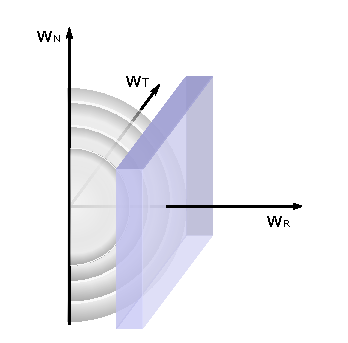
\includegraphics[width=.5\textwidth]{Figures/sketch_slice_R2.pdf}
	\centering
	\caption{Sketch of the orientation of a slice in the $w_T - w_N$ plane. A selection of ESA shells is shown in grey.}
	\label{fig:sketch_slice_R}
\end{figure}
By dividing these counts by the integrated phase space volume (PSV) for the observed time, which is binned in the same way and shown in Fig. \ref{fig:norm_50}, we obtain the resulting phase space density (PSD), s. Fig. \ref{fig:psd_50}. When comparing the three Figures \ref{fig:counts_50}, \ref{fig:norm_50} and \ref{fig:psd_50} one can see a clear difference in overall shape between PSV and PSD (resp. counts). The nonzero part of the PSD does not cover all of the scanned PSV. This means that SWICS did not observe $\mathrm{He^{+}}$ PUI over all of the observed PSV but only in a distinct partial volume.\\ 
However, the 2D projection of the PSD has a roundish shape. In fact we even find a spherical shape in 3D. As a feasible visualization a stepwise sequence of $w_\mathrm{sw,T} - w_\mathrm{sw,N}$ ``slices'' is displayed in Appendix \ref{Appendix}. Each slice is again a projection of the PSD from a width $\Delta w_\mathrm{sw,R} = 0.2$. The sequence starts with $w_\mathrm{sw,R}$-values below solar wind speed with the slice $-0.5 <= w_\mathrm{sw,R} < -0.3$ and steps seamlessly up to $1.1 <= w_\mathrm{sw,R} < 1.3$ in nine increments. The radius of the projection increases slightly towards $ w_\mathrm{sw,R} \approx 0$ and then starts decreasing again for larger $w_\mathrm{sw,R}$. This suggests the three-dimensional shape of a sphere centered around $w_\mathrm{sw,R} = 0$, which is a finding that confirms the theory of an isotopic and cooled PUI VDF (s. Sec. \ref{sec:theo_vdf}). \\
For $w_\mathrm{sw,R} < 0$ and towards smaller values of $w_\mathrm{sw,R}$ an increasing ``hole'' in the PSD emerges from the center. This is due to a limited instrumental coverage for $\mathrm{He^{+}}$ at higher ESA steps, which is described in more detail in Sec. \ref{subsec:cov}. \\
Apart from taking slices from the $w_\mathrm{sw,T} - w_\mathrm{sw,N}$ plane along the $w_\mathrm{sw,R}$-axis we can also cut the three-dimensional distribution of the PSD along the other two axes. This is shown for the $w_\mathrm{sw,R} - w_\mathrm{sw,N}$ plane in Fig. \ref{fig:sketch_slice_T} and for the the $w_\mathrm{sw,R} - w_\mathrm{sw,T}$ plane in Fig. \ref{fig:sketch_slice_N}, each projection containing $w_\mathrm{sw,R} = 0$.
Both images confirm the underlying three-dimensional spherical distribution.
\\
Taking a look at the $w_\mathrm{sw,R}$-slice of the PSV in Fig. \ref{fig:norm_50} again, one sees a relatively sharp peak in the bins around $w_\mathrm{sw,T} = 0.4$ and $w_\mathrm{sw,N} = 0$. This means that this part of PSV has been observed more often than surrounding parts, which is due to the spacecraft having a substantial aspect angle $\varphi_{asp}$ at the end of the year 1993 (s. Fig. \ref{fig:aa}). Because the spacecraft's spin axis was tilted away from the radial direction for most of the time, this peak is shifted a little bit away from the center. The fact that this distinct part of PSV has been observed particularly often coincides with a qualitatively similar peak in counts, s. Fig. \ref{fig:counts_50}. 
As this peak is a result of the measurement and not a feature in the velocity distribution of $\mathrm{He^{+}}$, it vanishes with the normalization process. The PSD shows an increased density over a wider range around the radial direction, which implies that $\mathrm{He^{+}}$ tends to stream radially in this example from 1993.
\begin{figure}[h]
	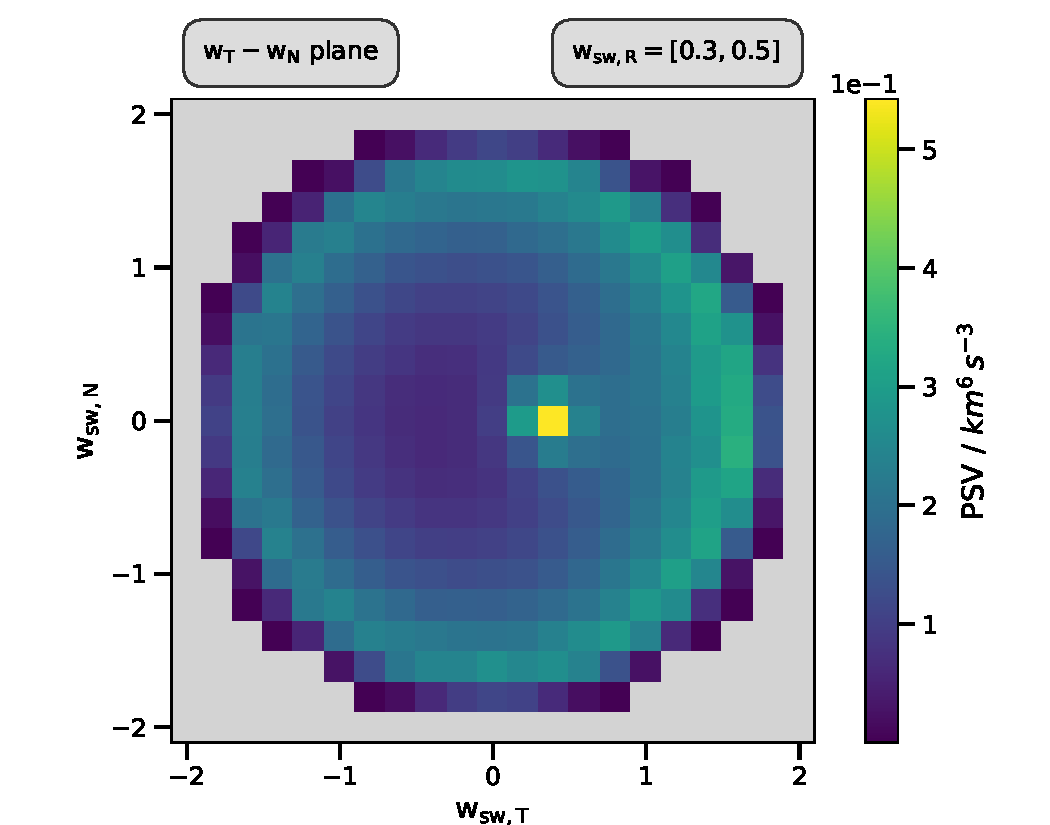
\includegraphics[width=.85\textwidth]{Figures/slice_50_norm.pdf}
	\centering
	\caption{Cartesian cut through the integrated observed PSV in a 3D $w_\mathrm{sw}$-space, measured during DOY 315-365 in 1993 for solar wind speeds from $760 \, \mathrm{km\,s^{-1}}$ to $780 \, \mathrm{km\,s^{-1}}$.}
	\label{fig:norm_50}
\end{figure}
\begin{figure}[h]
	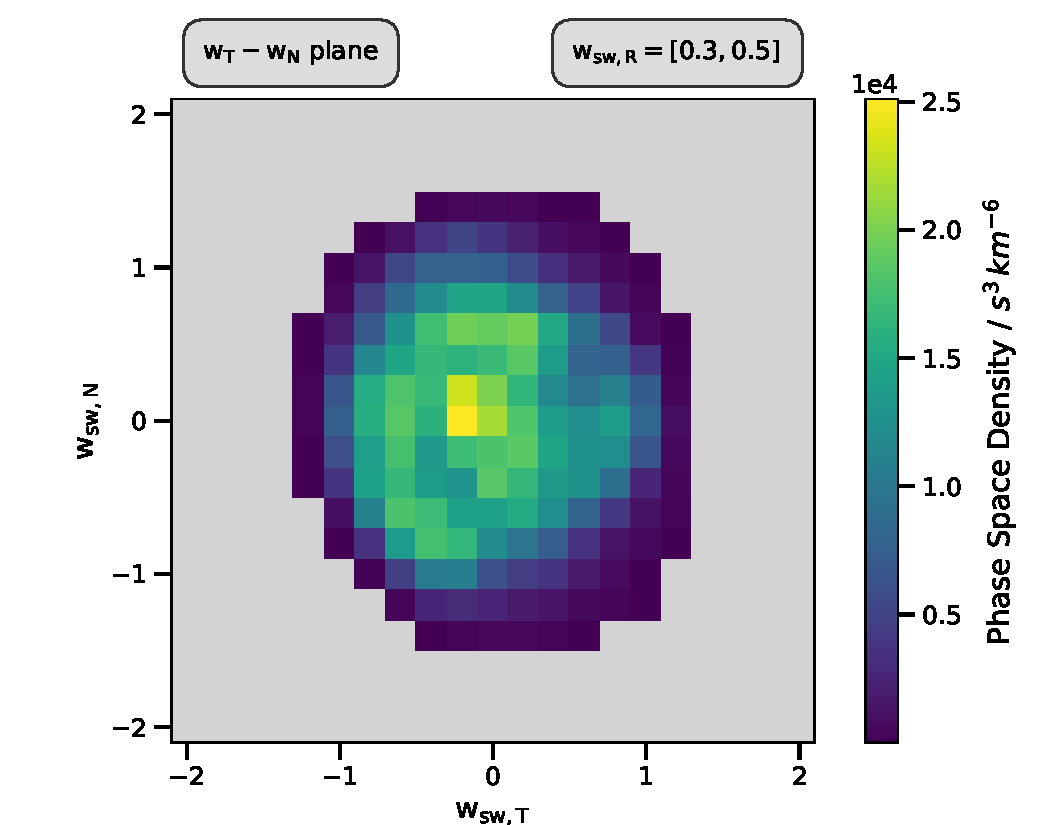
\includegraphics[width=.85\textwidth]{Figures/slices_50_3.pdf}
	\centering
	\caption{Cartesian cut through the three-dimensional PSD for $\mathrm{He^{+}}$, measured during DOY 315-365 in 1993 for solar wind speeds from $760 \, \mathrm{km\,s^{-1}}$ to $780 \, \mathrm{km\,s^{-1}}$}
	\label{fig:psd_50}
\end{figure}
% Skizzen / andere Slices:
\begin{figure}[h]
	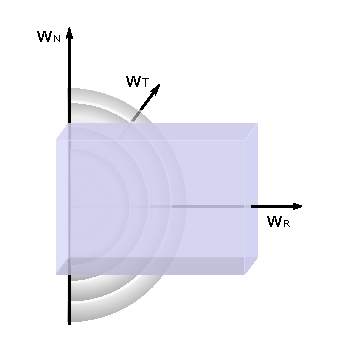
\includegraphics[width=.34\textwidth]{Figures/sketch_slice_T2.pdf}
	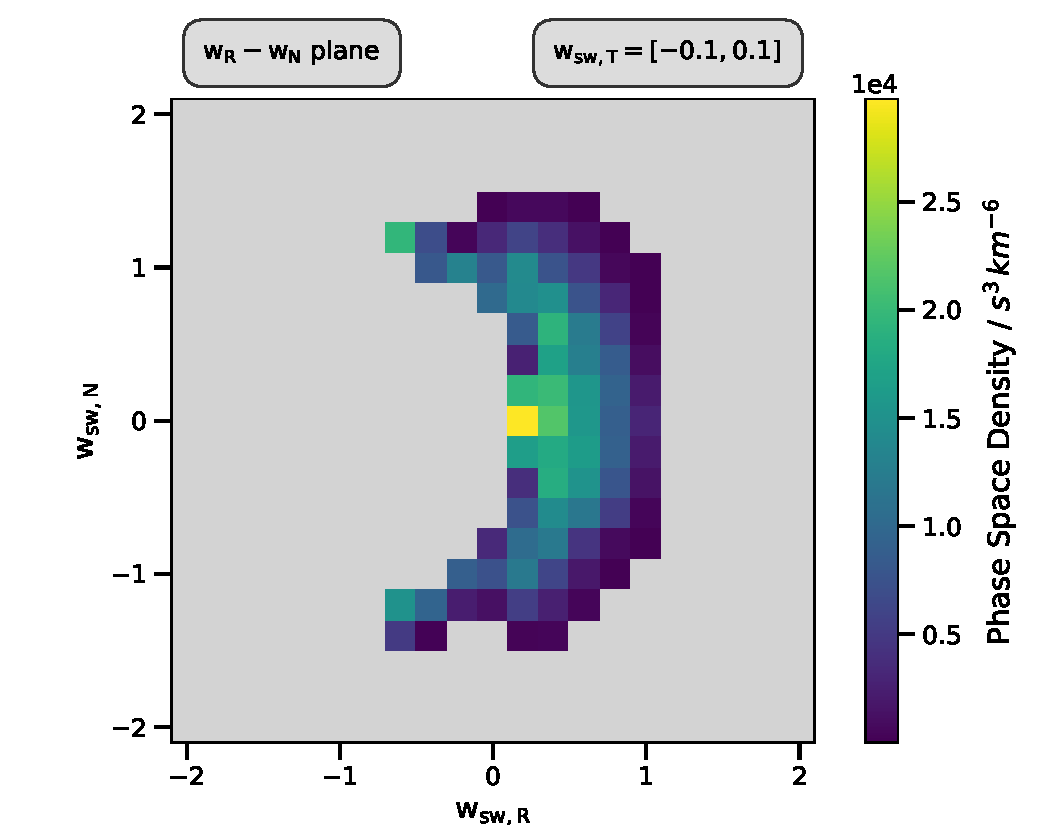
\includegraphics[width=.64\textwidth]{Figures/slice_50_T.pdf}
	\centering
	\caption{\textbf{Left:} Sketch of the orientation of a slice in the $w_R - w_N$ plane. A selection of ESA shells is shown in grey.\\ \textbf{Right:} Cartesian cut through the three-dimensional PSD for $\mathrm{He^{+}}$, measured during DOY 315-365 in 1993 for solar wind speeds from $760 \, \mathrm{km\,s^{-1}}$ to $780 \, \mathrm{km\,s^{-1}}$. The crescent shape results from SWICS' coverage.}
	\label{fig:sketch_slice_T}
\end{figure}
\begin{figure}[h]
	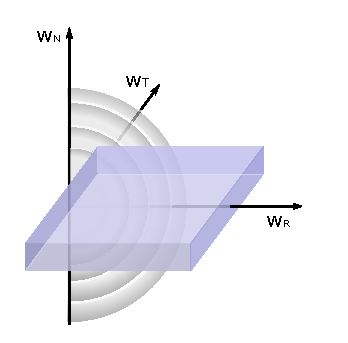
\includegraphics[width=.34\textwidth]{Figures/sketch_slice_N2.pdf}
	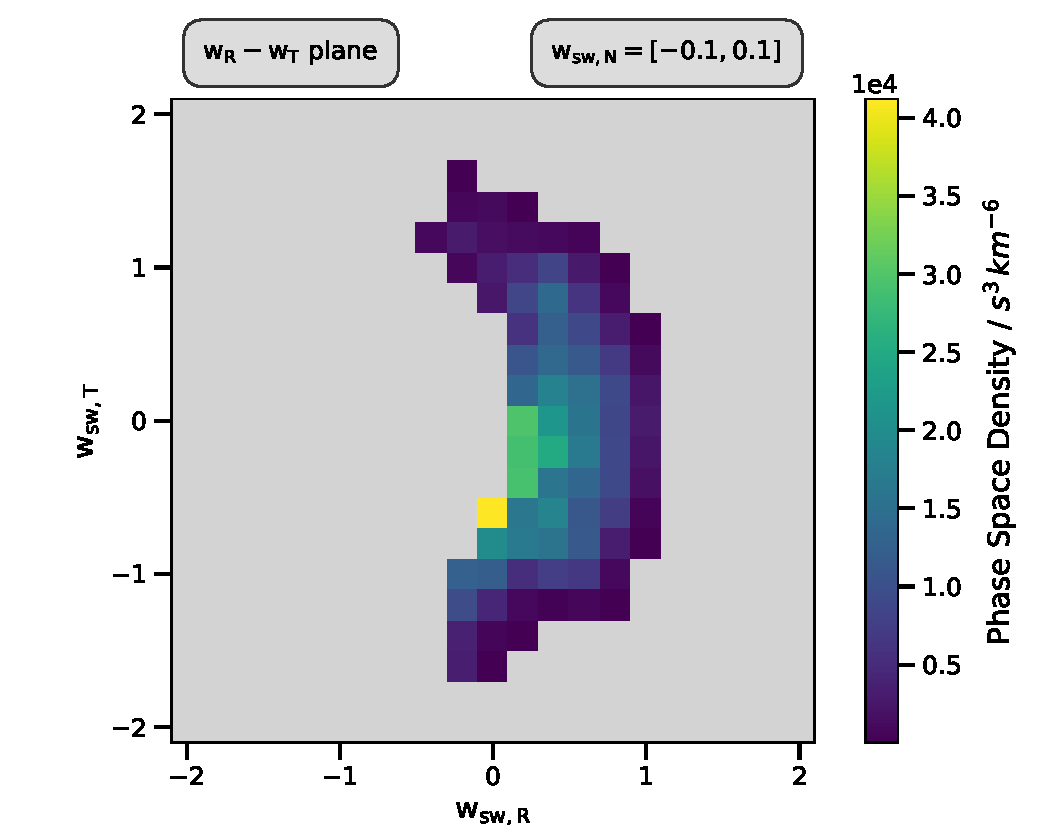
\includegraphics[width=.64\textwidth]{Figures/slice_50_N.pdf}
	\centering
	\caption{\textbf{Left:} Sketch of the orientation of a slice in the $w_R - w_T$ plane. A selection of ESA shells is shown in grey.\\ \textbf{Right:} Cartesian cut through the three-dimensional PSD for $\mathrm{He^{+}}$, measured during DOY 315-365 in 1993 for solar wind speeds from $760 \, \mathrm{km\,s^{-1}}$ to $780 \, \mathrm{km\,s^{-1}}$. The crescent shape results from SWICS' coverage.}
	\label{fig:sketch_slice_N}
\end{figure}
%
%
%
%
%
\clearpage
\noindent In Fig. \ref{fig:psd_lang} we show the PSD for another, longer, time period of 250 days in 1994 at solar wind speeds from $740 \, \mathrm{km\,s^{-1}}$ to $780 \, \mathrm{km\,s^{-1}}$ for a slice $0.1 <= w_\mathrm{sw,R} < 0.3$. Corresponding counts and PSV are shown in Figs. \ref{fig:counts_long} and \ref{fig:norm_long}. Here, the counts show a ring structure which vanishes by normalization. 
The PSD in  Fig. \ref{fig:psd_lang} shows a distribution that is similar to the PSD from the shorter time period in 1993, concentrated and symmetrical around the central radial direction.
\begin{figure}[h]
	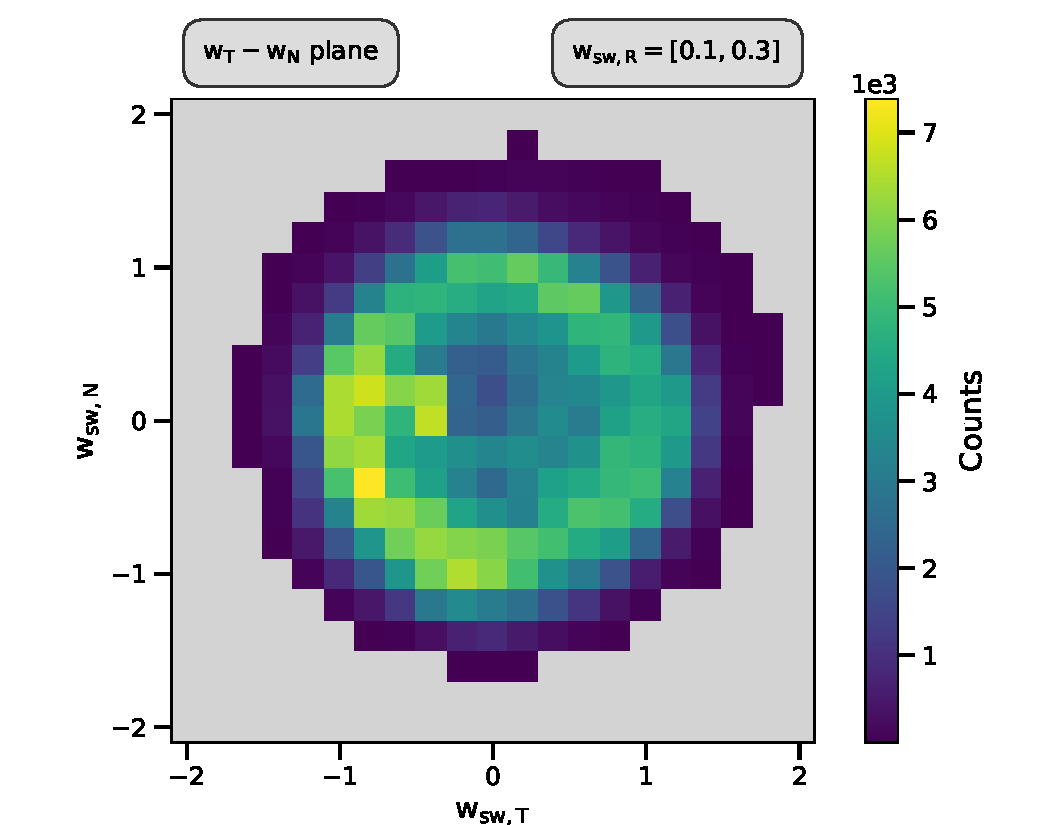
\includegraphics[width=.85\textwidth]{Figures/cart_long_counts.pdf}
	\centering
	\caption{Cartesian cut through $\mathrm{He^{+}}$ count distribution in a 3D $w_\mathrm{sw}$-space, measured during DOY 1-250 in 1994 for solar wind speeds from $740 \, \mathrm{km\,s^{-1}}$ to $780 \, \mathrm{km\,s^{-1}}$.}
	\label{fig:counts_long}
\end{figure}
\begin{figure}[h]
	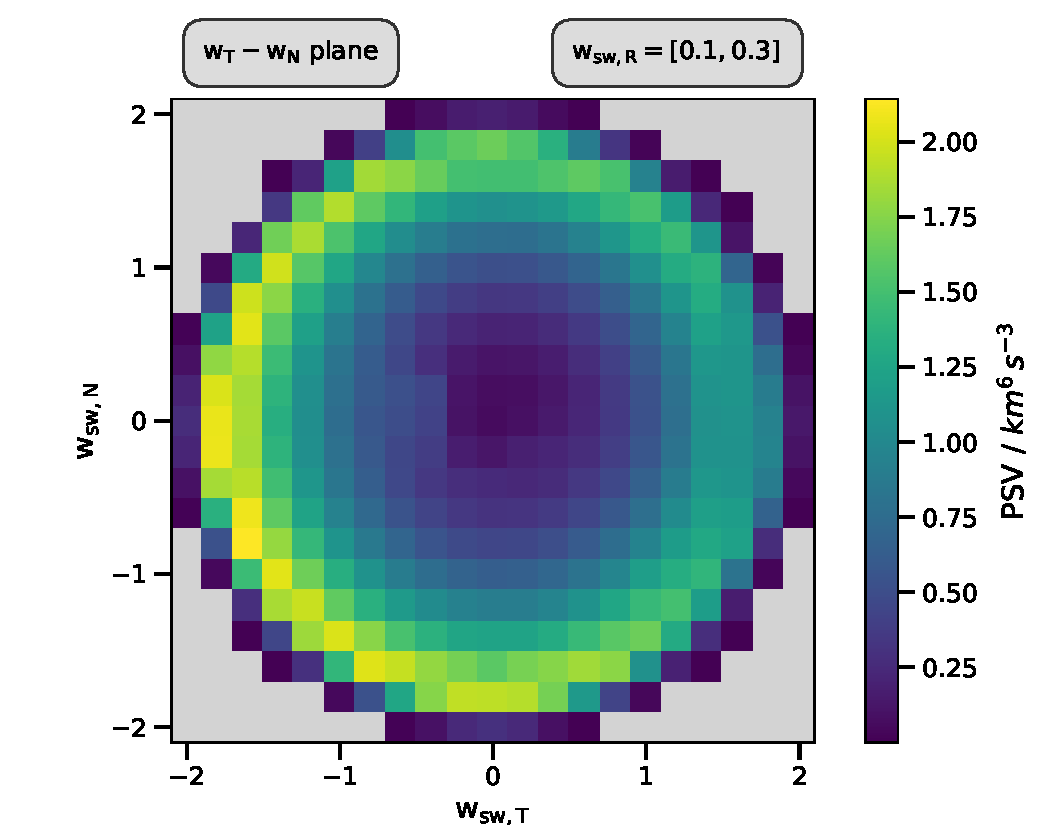
\includegraphics[width=.85\textwidth]{Figures/cart_long_norm.pdf}
	\centering
	\caption{Cartesian cut through the integrated observed PSV in a 3D $w_\mathrm{sw}$-space, measured during DOY 1-250 in 1994 for solar wind speeds from $740 \, \mathrm{km\,s^{-1}}$ to $780 \, \mathrm{km\,s^{-1}}$.}
	\label{fig:norm_long}
\end{figure}
\begin{figure}[h]
	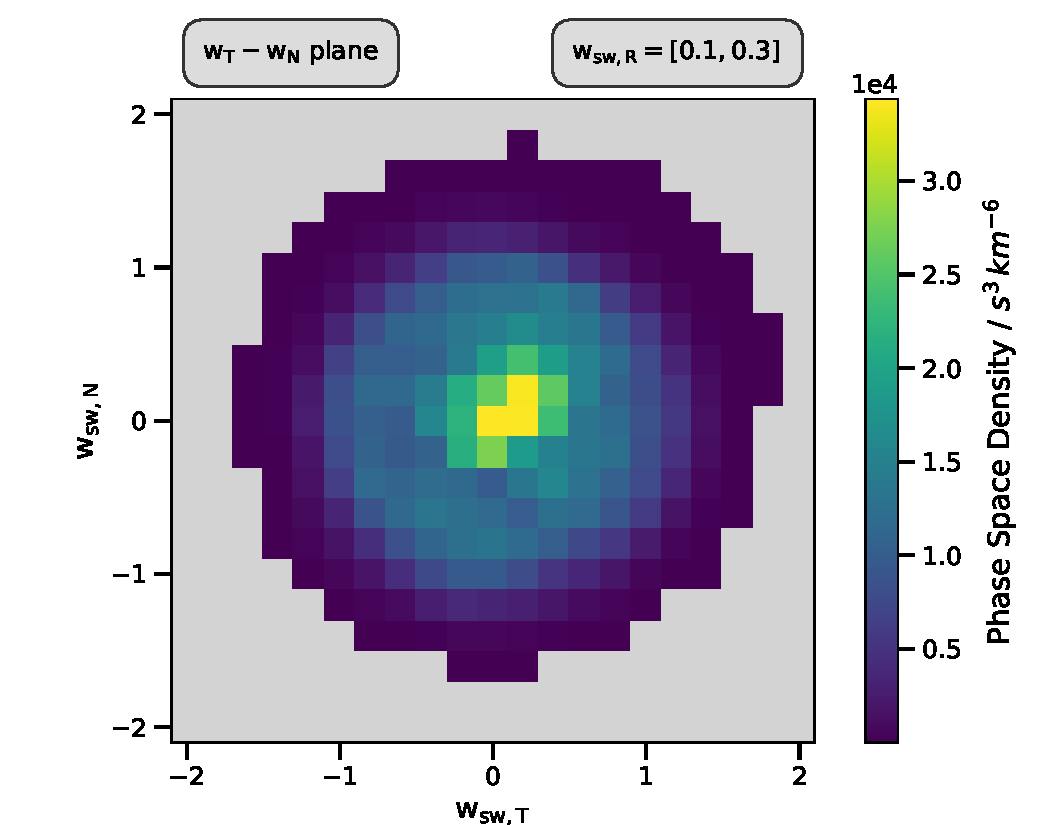
\includegraphics[width=.85\textwidth]{Figures/cart_long_ps.pdf}
	\centering
	\caption{Cartesian cut through the three-dimensional PSD for $\mathrm{He^{+}}$, measured during DOY 1-250 in 1994 for solar wind speeds from $740 \, \mathrm{km\,s^{-1}}$ to $780 \, \mathrm{km\,s^{-1}}$}
	\label{fig:psd_lang}
\end{figure}
%
%
%
%
%
\clearpage
\section{Spherical Projection}
Of course we are not limited to the so far presented Cartesian projections.
We can also choose a shell-wise projection. For this we consider spherical shells of constant $w_\mathrm{sw}$ in the solar wind frame. For better understanding we can refer to Fig. \ref{fig:cov} again. Here we see the blue rings as 2D cuts through such concentric shells around $w_\mathrm{sw} = 0$. The spherical coordinate $\varphi$ is measured within the $w_\mathrm{sw,T}-w_\mathrm{sw,N}$ plane with $\varphi = 0^\circ$ for $w_\mathrm{sw,T} = 0$ and $\varphi > 0^\circ$ for negative values of $w_\mathrm{sw,T}$. The second coordinate $\vartheta$ is defined perpendicular to the $w_\mathrm{sw,T}-w_\mathrm{sw,N}$ plane. It is $\vartheta = 0 ^\circ$ for values within the plane and $\vartheta = 90^\circ$ along the positive $w_\mathrm{sw,N}$ axis (out of the paper plane).
\\
In Figs. \ref{fig:sky_counts} and \ref{fig:sky_norm} we show counts and integrated PSV in this projection for $\mathrm{He^{+}}$ measurements from 50 days in 1993, restricted to solar wind speeds from $760 \, \mathrm{km\,s^{-1}}$ to $780 \, \mathrm{km\,s^{-1}}$. The selected spherical shell comprises absolute $w$ values $0.85 <= w_\mathrm{sw} < 0.95$. Considering the definition of the two coordinates $\varphi$ and $\vartheta$ we find that the central viewing direction is against the $w_\mathrm{sw,R}$-axis in Fig. \ref{fig:cov}. Even more clearly than in the Cartesian projection sharp peaks around $\varphi = 30 ^\circ$ and $\vartheta = 0 ^\circ$ are apparent in both figures \ref{fig:sky_counts} and \ref{fig:sky_norm}, which is due to the variation in observation time of PSV. The histogram of the corresponding PSD, which excludes this effect, is shown in Fig. \ref{fig:sky_psd}.\\
This spherical projection can become particularly suitable for the examination of the level of isotropy within a $w_\mathrm{sw}$-shell. Shapes like a torus distribution (s. Sec. \ref{sec:theo_vdf}) can be observed directly. For a completely isotropized shell we would expect an evenly colored projection in Fig. \ref{fig:sky_psd}. This is obviously not the case. Here, we find a structure of increased PSD that is around $-60\,^\circ$ longitude for $\vartheta = 0\,^\circ$ and moves towards $\varphi = 0\,^\circ$ for higher latitudes.
\\
Unfortunately, we could not find clear structures that were constant over different periods of measurement. A possible reason for that could be that we could only very vaguely determine the detection efficiency in Sec. \ref{subsec:det_eff}. As the spherical projection comprises measurements from different ESA steps (s. \ref{fig:cov}), an inaccurate efficiency weighting could either lead to a disappearance of real structures or even to an emerging of artificial ones. A detailed analysis of the detection efficiencies as it is shown in \citet{koeten} for ACE/SWICS is beyond the scope of this work but would be highly beneficial for future analyses.
\begin{figure}[h]
	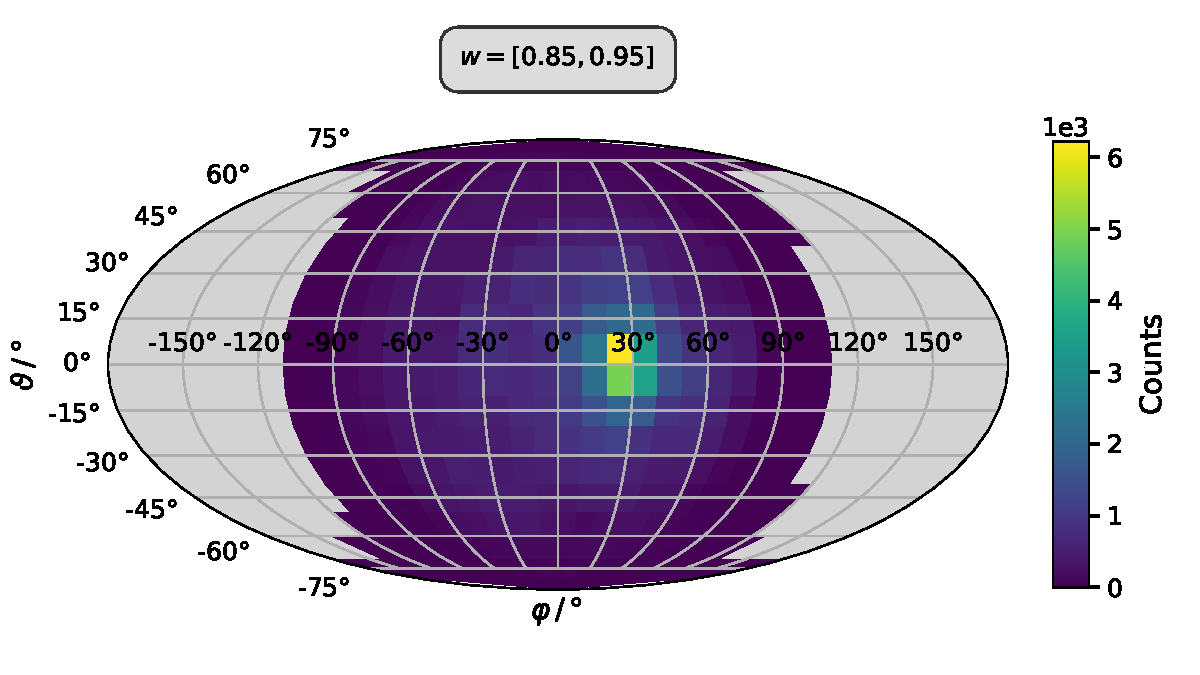
\includegraphics[width=1\textwidth]{Figures/sky_counts.pdf}
	\centering
	\caption{Spherical projection of $\mathrm{He^{+}}$ count distribution in a 3D $w_\mathrm{sw}$-space, measured during DOY 315-365 in 1993 for solar wind speeds from $760 \, \mathrm{km\,s^{-1}}$ to $780 \, \mathrm{km\,s^{-1}}$. Grey areas depict PSV (s. Fig \ref{fig:sky_norm}) that has not been observed and result from SWICS' coverage.}
	\label{fig:sky_counts}
\end{figure}
\begin{figure}[h]
	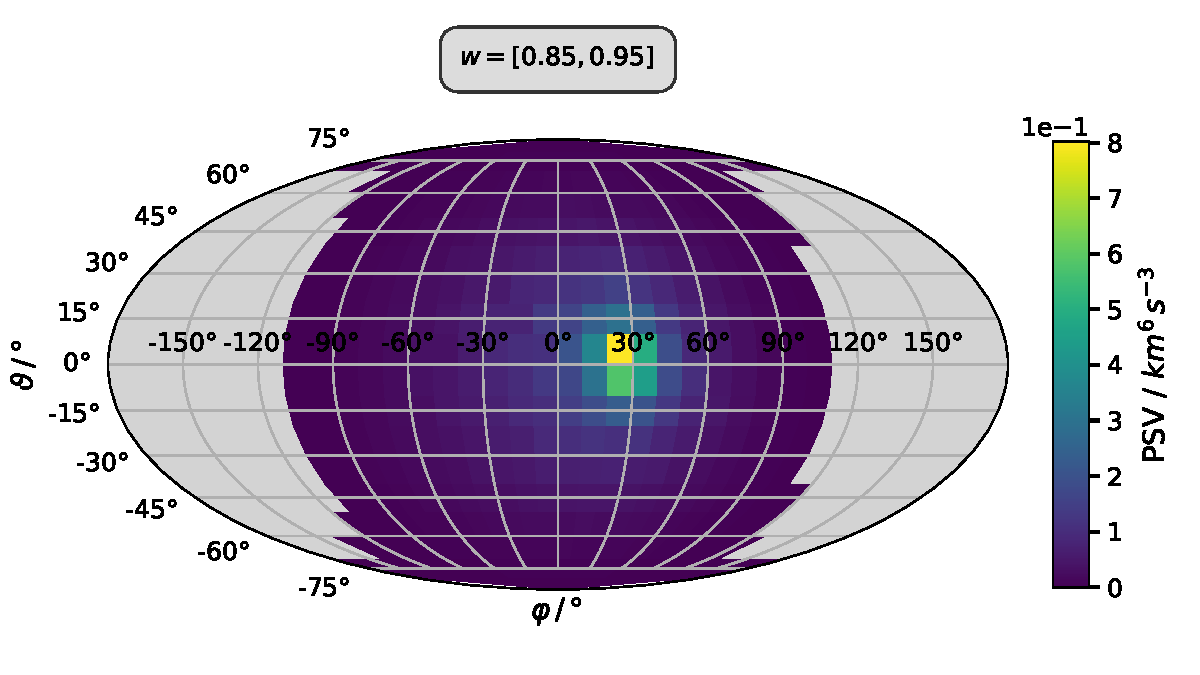
\includegraphics[width=1\textwidth]{Figures/sky_norm.pdf}
	\centering
	\caption{Spherical projection of the integrated observed PSV in a 3D $w_\mathrm{sw}$-space, measured during DOY 315-365 in 1993 for solar wind speeds from $760 \, \mathrm{km\,s^{-1}}$ to $780 \, \mathrm{km\,s^{-1}}$. Grey areas depict PSV that has not been observed and result from SWICS' coverage.}
	\label{fig:sky_norm}
\end{figure}
\begin{figure}[h]
	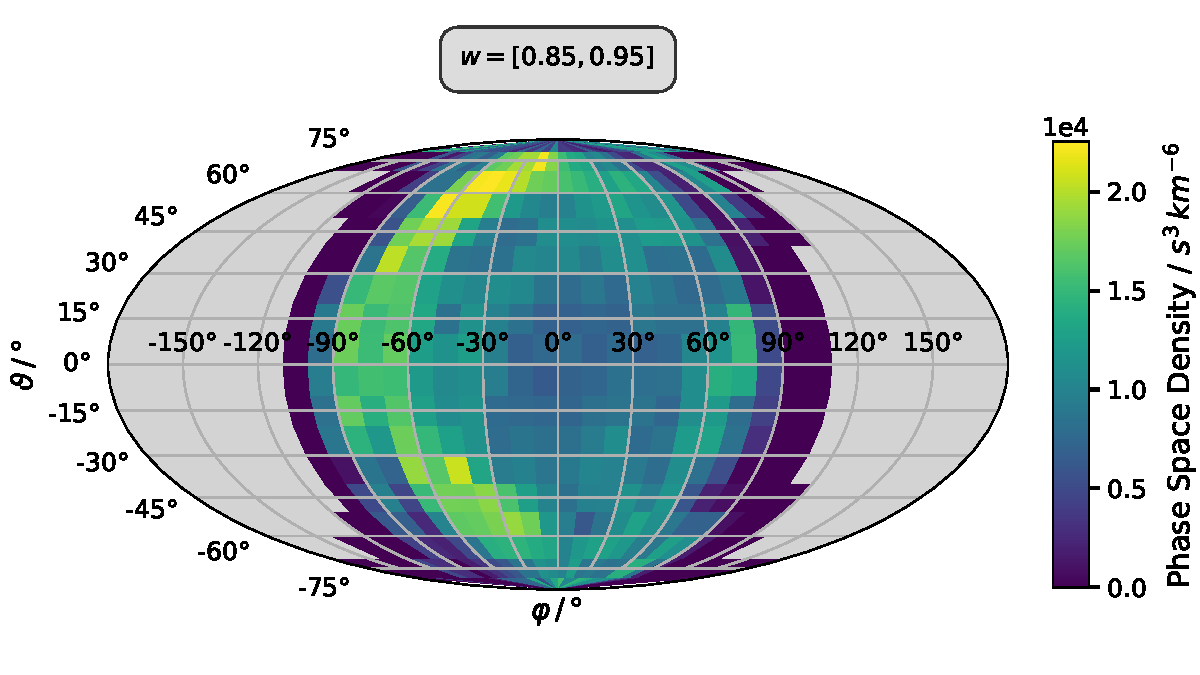
\includegraphics[width=1\textwidth]{Figures/sky_ps.pdf}
	\centering
	\caption{Spherical projection of the three-dimensional PSD for $\mathrm{He^{+}}$, measured during DOY 315-365 in 1993 for solar wind speeds from $760 \, \mathrm{km\,s^{-1}}$ to $780 \, \mathrm{km\,s^{-1}}$. Grey areas depict PSV (s. Fig \ref{fig:sky_norm}) that has not been observed and result from SWICS' coverage.}
	\label{fig:sky_psd}
\end{figure}
%
%
%
\clearpage
\section{1D Projection}
In this last section we show 1D projections of three-dimensional velocity distributions from measurements taken in two different years. In each year (1993, 1996) we analyzed $\mathrm{He^{+}}$ data from 100 days at solar wind speeds from $760 \, \mathrm{km\,s^{-1}}$ to $770 \, \mathrm{km\,s^{-1}}$.\\
For this projection we integrate both the counts and the PSV over spherical shells around $w_\mathrm{sw}=0$. In a 2D cut this can be visualized by an integration along a blue circle in Fig. \ref{fig:cov}. We combine values within the width $\Delta w_\mathrm{sw} = 0.1$ at different radii from $w_\mathrm{sw} = 0.25$ to $w_\mathrm{sw} = 1.05$. In Fig. \ref{fig:1d} the histogram of the resulting PSD is shown. The histograms look qualitatively similar for both years. 
We see a relatively broad distribution with a clear cutoff around $w = 1$, which corresponds to $w_\mathrm{sc} = 2$ (s. Sec. \ref{sec:theo_vdf}, Ch. \ref{chap:intro}). For smaller values of $w_\mathrm{sw}$ the distribution does not change over many magnitudes. 
\\
The spectra in Fig. \ref{fig:1d} are also in good qualitative agreement with the one in Fig. \ref{fig:gloeckler}. It should be noted that our spectra are limited to values $w_\mathrm{sw} > 0.25$, while the spectrum in Fig. \ref{fig:gloeckler} is continued down to values $w_\mathrm{sc} < 1$, which corresponds to values $w_\mathrm{sw} < 0$ in solar wind frame. In Sec. \ref{subsec:cov} we have seen that $\mathrm{He^{+}}$ Triple Coincidences can only be measured for distinct $w$ values above a limit that is dependent on the solar wind speed but hardly smaller than $w_\mathrm{sw} = 1$. This shows that the spectrum in Fig. \ref{fig:gloeckler} is not based on solely Triple Coincidences but also on $\mathrm{He^{+}}$ Double Coincidences. As Double Coincidences lack an energy measurement in the solid-state detector and thus a directional resolution, the spectrum can only result from an integration along different ESA shells that is projected onto a distinct possible value.
Although the spectra look similar we want to emphasize that the spectrum in Fig. \ref{fig:1d} results from a very different approach as we show projected cuts through an actual three-dimensional velocity distribution.
\begin{figure}[h]
	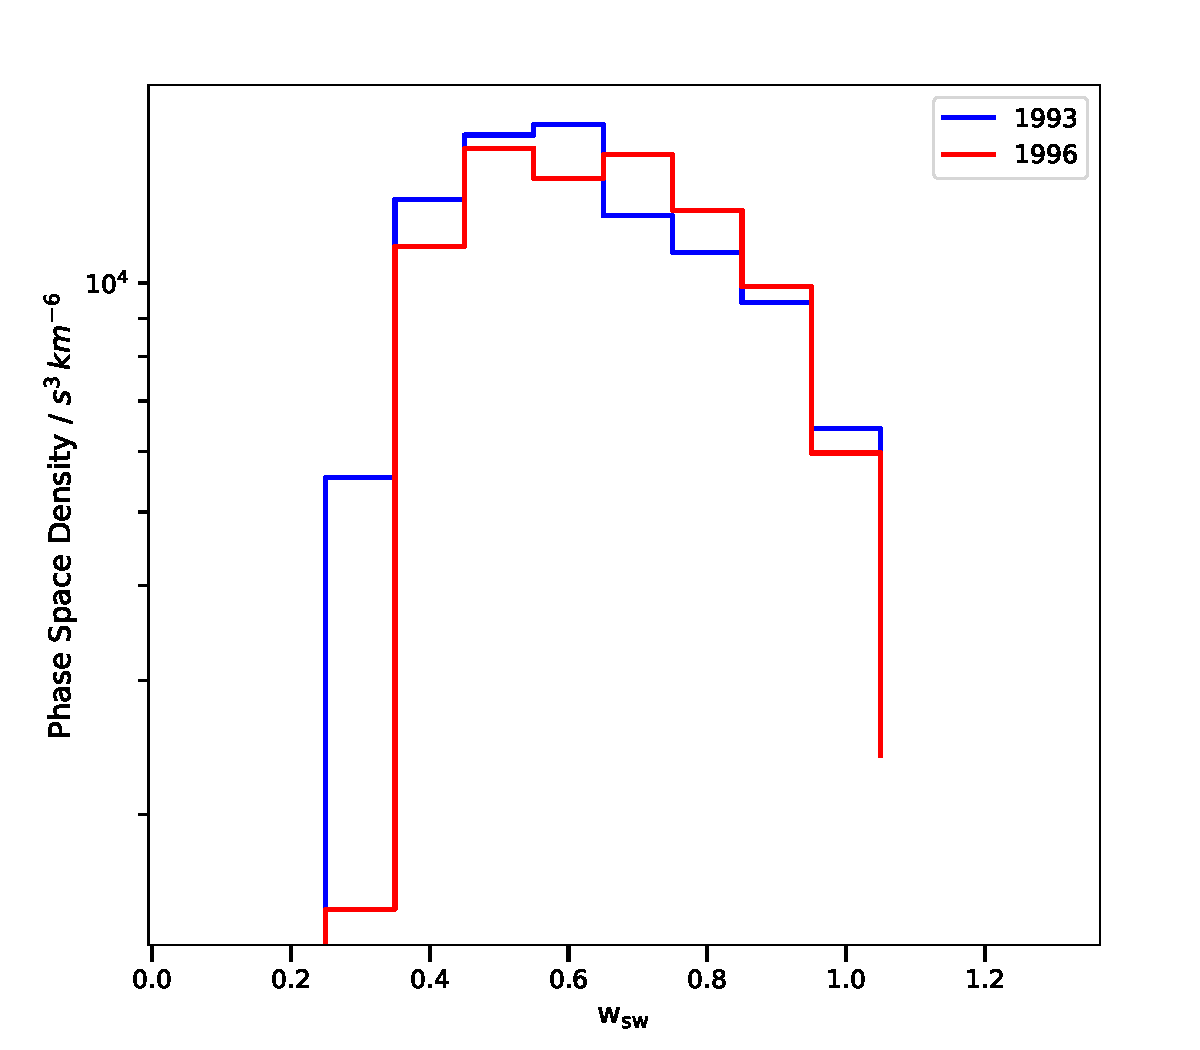
\includegraphics[width=.8\textwidth]{Figures/1D.pdf}
	\centering
	\caption{1D projected PSD from a 3D $w_\mathrm{sw}$-space, measured during DOY 1-100 in 1994 and 1996 for solar wind speeds from $760 \, \mathrm{km\,s^{-1}}$ to $770 \, \mathrm{km\,s^{-1}}$.}
	\label{fig:1d}
\end{figure} 
% Chapter Template

\chapter{Conclusion} % Main chapter title

\label{chap:concl} % Change X to a consecutive number; for referencing this chapter elsewhere, use \ref{ChapterX}

 

%----------------------------------------------------------------------------------------
%	THESIS CONTENT - APPENDICES
%----------------------------------------------------------------------------------------

\appendix % Cue to tell LaTeX that the following "chapters" are Appendices

% Include the appendices of the thesis as separate files from the Appendices folder
% Uncomment the lines as you write the Appendices
% Appendix Template

\chapter{Test} % Main appendix title

\label{AppendixX} % Change X to a consecutive letter; for referencing this appendix elsewhere, use \ref{AppendixX}

%%%%%%%%%%%%%%%%%%%%%%%%%%%


\begin{figure}[h]
	%\includegraphics[width=0.5\textwidth]{Figures/PLOT_EIGEN_VELOCITY.pdf}
	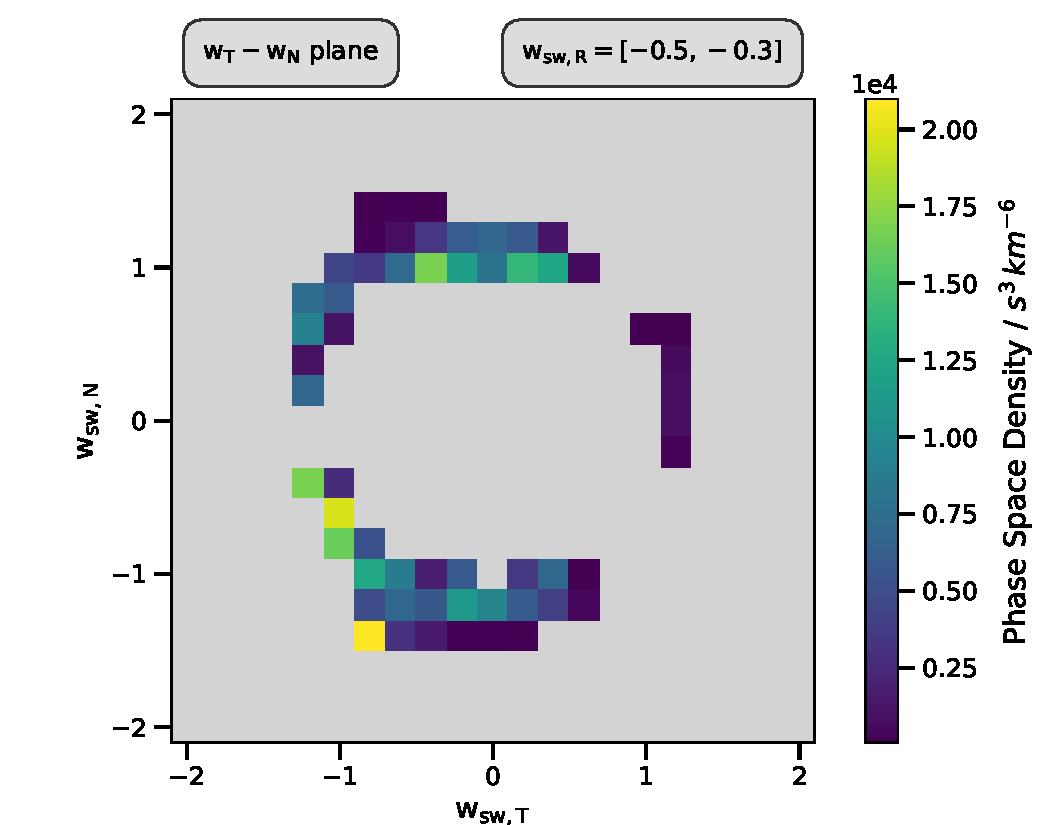
\includegraphics[width=1.\textwidth]{Figures/slices_50_-5.pdf}
	\centering
	\caption{todo}
	\label{fig:todo}
\end{figure}

\begin{figure}[h]
	%\includegraphics[width=0.5\textwidth]{Figures/PLOT_EIGEN_VELOCITY.pdf}
	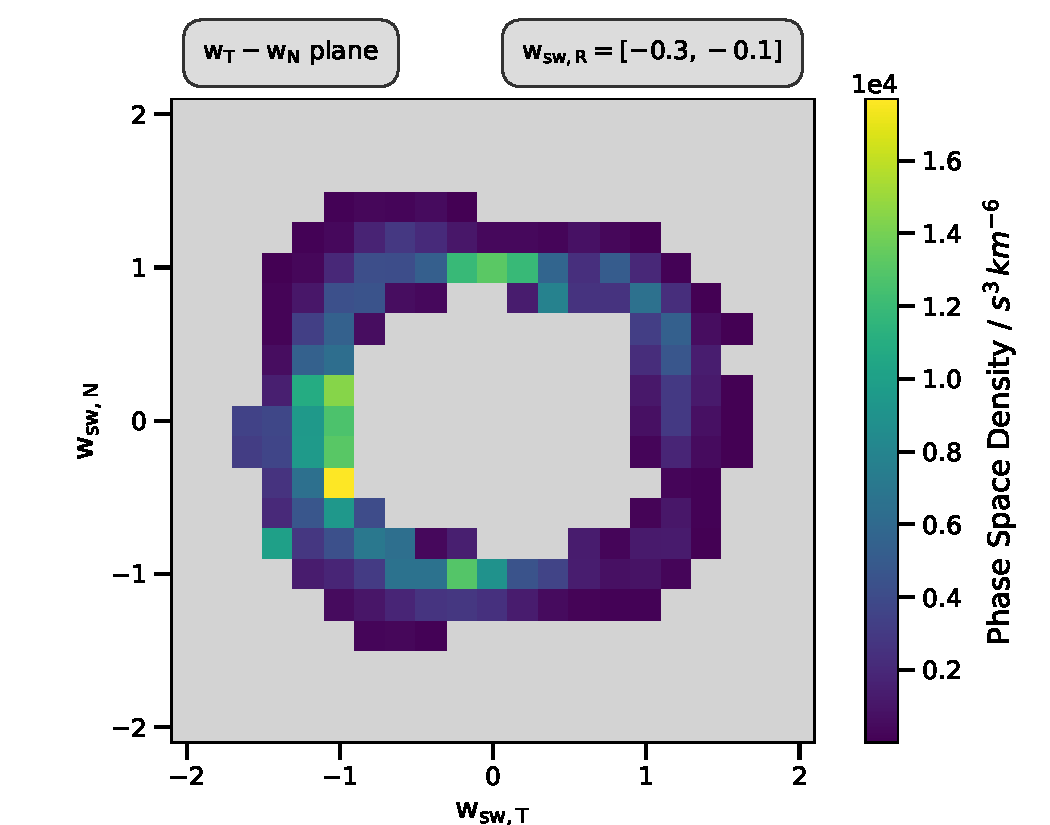
\includegraphics[width=1.\textwidth]{Figures/slices_50_-3.pdf}
	\centering
	\caption{todo}
	\label{fig:todo}
\end{figure}

\begin{figure}[h]
	%\includegraphics[width=0.5\textwidth]{Figures/PLOT_EIGEN_VELOCITY.pdf}
	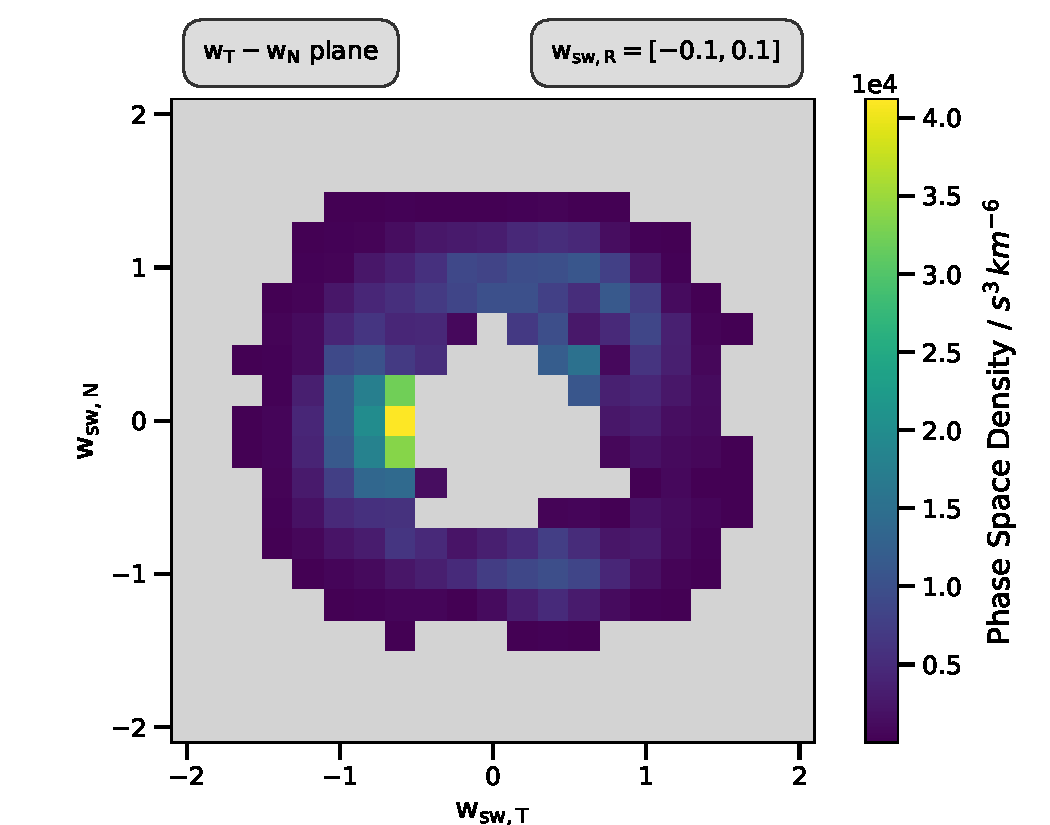
\includegraphics[width=1.\textwidth]{Figures/slices_50_-1.pdf}
	\centering
	\caption{todo}
	\label{fig:todo}
\end{figure}

\begin{figure}[h]
	%\includegraphics[width=0.5\textwidth]{Figures/PLOT_EIGEN_VELOCITY.pdf}
	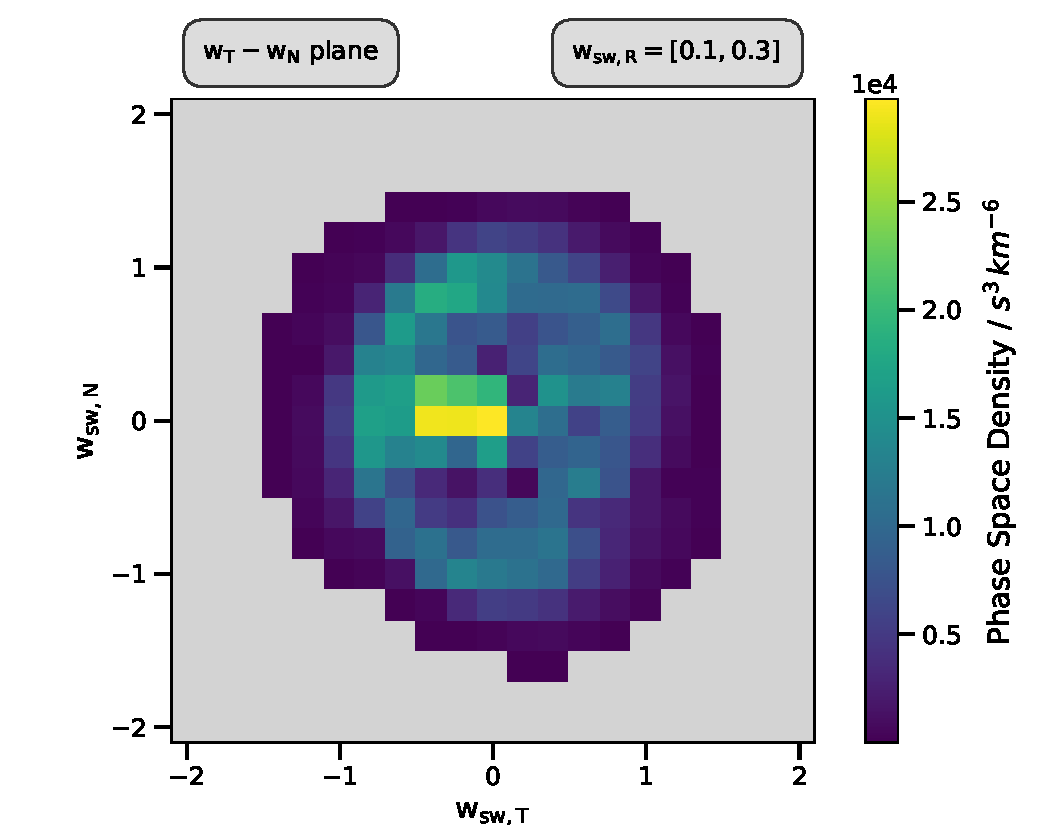
\includegraphics[width=1.\textwidth]{Figures/slices_50_1.pdf}
	\centering
	\caption{todo}
	\label{fig:todo}
\end{figure}

\begin{figure}[h]
	%\includegraphics[width=0.5\textwidth]{Figures/PLOT_EIGEN_VELOCITY.pdf}
	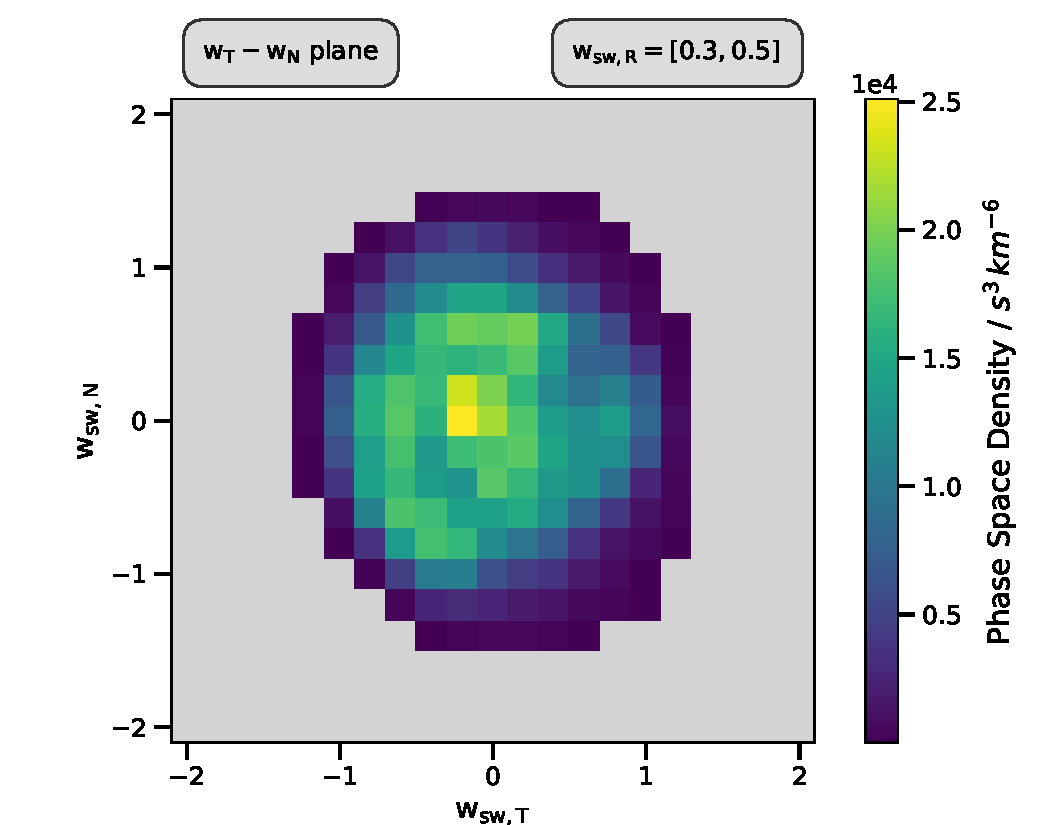
\includegraphics[width=1.\textwidth]{Figures/slices_50_3.pdf}
	\centering
	\caption{todo}
	\label{fig:todo}
\end{figure}

\begin{figure}[h]
	%\includegraphics[width=0.5\textwidth]{Figures/PLOT_EIGEN_VELOCITY.pdf}
	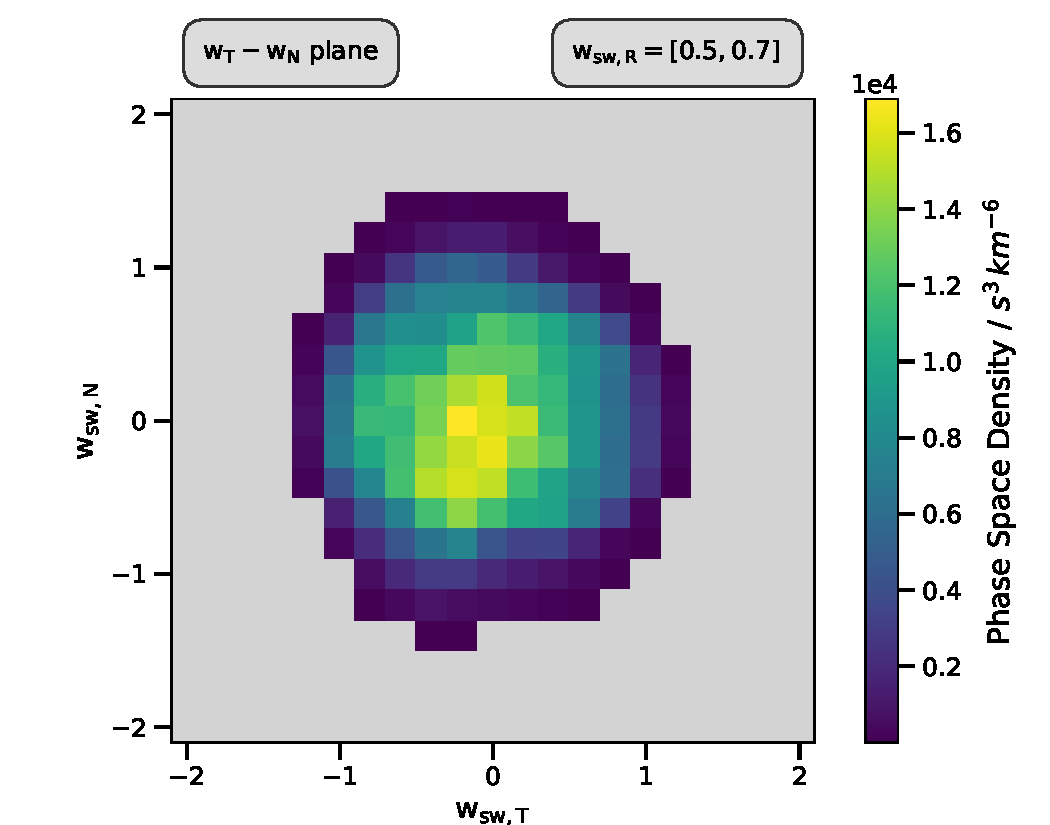
\includegraphics[width=1.\textwidth]{Figures/slices_50_5.pdf}
	\centering
	\caption{todo}
	\label{fig:todo}
\end{figure}

\begin{figure}[h]
	%\includegraphics[width=0.5\textwidth]{Figures/PLOT_EIGEN_VELOCITY.pdf}
	\includegraphics[width=1.\textwidth]{Figures/slices_50_7.pdf}
	\centering
	\caption{todo}
	\label{fig:todo}
\end{figure}

\begin{figure}[h]
	%\includegraphics[width=0.5\textwidth]{Figures/PLOT_EIGEN_VELOCITY.pdf}
	\includegraphics[width=1.\textwidth]{Figures/slices_50_9.pdf}
	\centering
	\caption{todo}
	\label{fig:todo}
\end{figure}

\begin{figure}[h]
	%\includegraphics[width=0.5\textwidth]{Figures/PLOT_EIGEN_VELOCITY.pdf}
	\includegraphics[width=1.\textwidth]{Figures/slices_50_11.pdf}
	\centering
	\caption{todo}
	\label{fig:todo}
\end{figure}


%% Appendix A

\chapter{Frequently Asked Questions} % Main appendix title

\label{AppendixA} % For referencing this appendix elsewhere, use \ref{AppendixA}

\section{How do I change the colors of links?}

The color of links can be changed to your liking using:

{\small\verb!\hypersetup{urlcolor=red}!}, or

{\small\verb!\hypersetup{citecolor=green}!}, or

{\small\verb!\hypersetup{allcolor=blue}!}.

\noindent If you want to completely hide the links, you can use:

{\small\verb!\hypersetup{allcolors=.}!}, or even better: 

{\small\verb!\hypersetup{hidelinks}!}.

\noindent If you want to have obvious links in the PDF but not the printed text, use:

{\small\verb!\hypersetup{colorlinks=false}!}.

%----------------------------------------------------------------------------------------
%	BIBLIOGRAPHY
%----------------------------------------------------------------------------------------

\printbibliography[heading=bibintoc]

%----------------------------------------------------------------------------------------


%----------------------------------------------------------------------------------------
%	DECLARATION PAGE
%----------------------------------------------------------------------------------------

\begin{declaration}
	\addchaptertocentry{\authorshipname} % Add the declaration to the table of contents

Hiermit erkläre ich, dass ich die vorliegende Masterarbeit selbständig und lediglich unter Benutzung der angegebenen Quellen und Hilfsmittel verfasst habe. Ferner versichere ich, dass die vorliegende Arbeit noch nicht im Rahmen eines anderen Prüfungsverfahrens eingereicht wurde. \\[1cm]
	
	\noindent Ort, Datum:\\
	\rule[0.5em]{25em}{0.5pt} % This prints a line for the signature
	\\[0.5cm]
	\noindent Unterschrift:\\
	\rule[0.5em]{25em}{0.5pt} % This prints a line to write the date
\end{declaration}


%----------------------------------------------------------------------------------------
%	ACKNOWLEDGEMENTS
%----------------------------------------------------------------------------------------

%\begin{acknowledgements}
%	\addchaptertocentry{\acknowledgementname} % Add the acknowledgements to the table of contents
%	The acknowledgments and the people to thank go here, don't forget to include your project advisor\ldots
%\end{acknowledgements}


\end{document}  
